\documentclass{kththesis}

%\usepackage{csquotes}
%\usepackage[style=numeric, sorting=none, backend=bibtex]{biblatex}
\usepackage[backend=bibtex, natbib=true, style=authoryear, dashed=false, maxbibnames=3, giveninits=true, uniquename=init]{biblatex}
\renewcommand{\citet}[1]{\citeauthor{#1} (\citeyear{#1})}
\newcommand{\citen}[1]{\citeauthor{#1}, \citeyear{#1}}

\usepackage{caption}
\captionsetup[figure]{font=footnotesize,labelfont=footnotesize}

\usepackage{threeparttable}

\usepackage[export]{adjustbox}[2011/08/13]
%\usepackage{algorithm}
%\usepackage{algorithmic}

%\usepackage{endfloat}

\addbibresource{../Literature/EasterIslandbib.bib}
%\def\citep\parentcite
\input{/home/peter/Organisatorisches/Latex_dinge/packages_kththesis}
\title{A Spatially Explicit Agent-Based Model of Human-Resource Interaction on Easter Island}
\alttitle{det är en svenska titlen}
\author{Peter Steiglechner}
\email{peter.steiglechner@gmail.com}
\supervisor{Agostino Merico}
\examiner{Michael Hanke}
\hostcompany{Leibniz Centre for Tropical Marine Research (ZMT)}
\programme{Master in Computer Simulations in Science and Engineering}
\school{School of Engineering Sciences}
\date{\today}

\kthcover{kth-cover.pdf}
\setcounter{tocdepth}{3}
\setcounter{secnumdepth}{3	}

\begin{document}
\frontmatter
%\begin{titlepage}
	\begin{center}
		\maketitle
	\end{center}
\end{titlepage}


\titlepage

\begin{abstract}
	% !TEX root=frame_thesis.tex

The history of Easter Island, with its cultural and ecological mysteries, has attracted the interests of archaeologists, anthropologists, ecologists, and econo\-mists alike. Despite the great scientific efforts, uncertainties in the available archaeological and palynological data leave a number of critical issues unsolved and open to debate. The maximum size reached by the human population before the arrival of Europeans and the temporal dynamics of deforestation are some of the aspects still fraught with controversies. By providing a quantitative workbench for testing hypotheses and scenarios, mathematical models are a valuable complement to the observational-based approaches generally used to reconstruct the history of the island. Previous modelling studies, however, have shown a number of shortcomings in the case of Easter Island, especially when they take no account of the stochastic nature of population growth in a temporally and spatially varying environment. Here, I present a new stochastic, Agent-Based Model characterised by (1) realistic physical geography of the island and other environmental constraints (2) individual agent decision-making processes, (3) non-ergodicity of agent behaviour and environment, and (4) randomised agent-environment interactions. I use the model and the best available data to determine plausible spatial and temporal patterns of deforestation and other socioecological features of Easter Island prior to the European contact.% and provide a general proof of concept of the model.
I further identify some non-trivial connections between microscopic decisions or constraints (like local confinement of agents' actions or their adaption strategy to environmental degradation) and macroscopic behaviour of the system that can not easily be neglected in a discussion about the history of Easter Island.
\end{abstract}
\begin{otherlanguage}{swedish}
\end{otherlanguage}
%\newpage 

\tableofcontents

\mainmatter
%% !TEX root=frame_thesis.tex

The history of Easter Island, with its cultural and ecological mysteries, has attracted the interests of archaeologists, anthropologists, ecologists, and econo\-mists alike. Despite the great scientific efforts, uncertainties in the available archaeological and palynological data leave a number of critical issues unsolved and open to debate. The maximum size reached by the human population before the arrival of Europeans and the temporal dynamics of deforestation are some of the aspects still fraught with controversies. By providing a quantitative workbench for testing hypotheses and scenarios, mathematical models are a valuable complement to the observational-based approaches generally used to reconstruct the history of the island. Previous modelling studies, however, have shown a number of shortcomings in the case of Easter Island, especially when they take no account of the stochastic nature of population growth in a temporally and spatially varying environment. Here, I present a new stochastic, Agent-Based Model characterised by (1) realistic physical geography of the island and other environmental constraints (2) individual agent decision-making processes, (3) non-ergodicity of agent behaviour and environment, and (4) randomised agent-environment interactions. I use the model and the best available data to determine plausible spatial and temporal patterns of deforestation and other socioecological features of Easter Island prior to the European contact.% and provide a general proof of concept of the model.
I further identify some non-trivial connections between microscopic decisions or constraints (like local confinement of agents' actions or their adaption strategy to environmental degradation) and macroscopic behaviour of the system that can not easily be neglected in a discussion about the history of Easter Island.

% !TEX root=frame_thesis.tex

\chapter{Introduction}


%First resource are trees, which were cut and used for food production (sweet sap is emerging from cut stems \citet{Mieth2015}), the production of manufactured goods like ropes or tools as well as canoes for fishing, firewood for cooking and cremation and, not to forget, the construction and transport of the Moai (e.g.\ \citet{Diamond2011}). Due to the slow regrowth of the palm tree (e.g. \citet{Brander1998}) this resource is close to non-renewable. Furthermore, the Polynesian rat, introduced by the first settlers at least stopped regrowth of the tree






%Easter Island's suitability for agriculture has been subject to excessive debate not least due to the first very contrary observations made by Roggeveen in 1722 as an `outstandingly fruitful' and by Cook in 1774 as an extremely poor and often sterile island \citep{Bahn2017}. %page 112   % who perceived the island's agricultural potential completely contrary \citep{Cauwe2011}.
%Nevertheless, from archaeological studies we know that the Easter Island people cultivated sweet potato, taro, yam, banans, sugar cane and other crops.
%Since sweet potato appears to be the dominant staple crop \citep{Louwagie2006}, I focus on this single crop here.

%Despite the progress so far, hypothesis  have produced very different results with strong implications on the reconstructed history of the Rapa Nui.

\section{The dispute about pre-historic Easter Island}

\begin{itemize}
	\item Easter Island's Pre-history is a fiercely debated topic
	\item Different theories exist on the population dynamics \citet{Hunt2007} and \citet{Diamond2011}/\citet{Bahn2017}.
	\item The differences occur because archaeological data is connected to large uncertainties (e.g.\ tree patterns \citet{Rull2020})
	\item Mathematical modelling has helped to explain possible scenarios of the dynamics and give interpretations of the historical developments.
	\item So far, all mathematical models focus on differential equation based approaches for the aggregate population of Easter Island.
	\item \citet{Brander1998}
	\item Variations of \citet{Brander1998}: Summarise the reviews in \citet{Reuveny2012}, \citet{Merico2017}.
	\item Social institution Extension of \citet{Brander1998}: \citet{Good2006}.
	\item Spatial Diffusion and Rats extension of \citet{Brander1998}: \citet{Basener2008}.
	\item The problem of these models is that with little variation in the parameters, any population dynamics can be achieved \citep{Brandt2015}.
\end{itemize}

\section{Agent Based Modelling of human resource interactions}
\begin{itemize}
\item What is Agent Based Modelling
\item The basic structure of an ABM in human resource interactions: Agents in environment, Update all agents asynchronously, update environment. Within each update agents change their local environment and their behaviour/properties are in turn influenced by the local environment. 
\item It breaks with ODE-type of modeling because it enables: 
\begin{itemize}
	\item spatially explicit modelling,
	\item  emergent global behaviour from local rules, 
	\item computational irreducibility of agent behaviour in terms of crisis. 
	\item Non-ergodic relation between agents and their environment.
	\item Stochasticity is natural in the decision making process, due to an agent's imperfect knowledge of the global sitution
\end{itemize}
\item ABM in ancient historical population dynamics: Maya \citep{Heckbert2013} and Anasazi \citep{Axtell2002}
\item Why ABM could help in Easter Island modelling: \citet{Merico2017}.
\item Structure of this thesis.
\end{itemize}


% !TEX root=frame_thesis.tex

\chapter{Mathematical Theory}\label{chapter:Theory}
\FloatBarrier
\section{Differential Equation Based Approaches for Easter Island}
%\begin{itemize}
%	\item Mathematical modelling has helped to explain possible scenarios of the dynamics and give interpretations of the historical developments.
%	\item So far, all mathematical models focus on differential equation based approaches for the aggregate population of Easter Island.
%	\item \citet{Brander1998}
%	\item Variations of \citet{Brander1998}: Summarise the reviews in \citet{Reuveny2012}, \citet{Merico2017}.
%	\item Social institution Extension of \citet{Brander1998}: \citet{Good2006}.
%	\item Spatial Diffusion and Rats extension of \citet{Brander1998}: \citet{Basener2008}.
%	\item The problem of these models is that with little variation in the parameters, any population dynamics can be achieved \citep{Brandt2015}.
%\end{itemize}

\paragraph{The Basic Ordinary Differential Equation Model.}
Theories on the population dynamics and deforestation on Easter Island are typically supported by a mathematical, human-resource interaction model.
%By making assumptions about these interaction sometimes based on archaeological data, these models can produce realistic population dynamics and thereby explain or rule out certain scenarios under the used set of assumptions. 
So far, all these models are based on aggregate predator-prey type of interaction between humans and resources (so called Lotka-Volterra model).
The dynamics of these macroscopic variables is then described by non-linear, coupled ordinary differential equations (ODEs).
The first and most famous model was developed by \citet{Brander1998}. 
The authors simulate the dynamics of two variables, a growing human population $L$ (the predator) and a logistically growing, open-access resource with stock $S$ (the prey).
This resource can be interpreted as the forest/soil complex, which is slowly renewable in this model. 
Of course, the Rapa Nui did not live off trees but they provided valuable derivate products or ecosystem services e.g.\ as habitat for birds, firewood, wood for tools or the transport of the Moai statues, or even for extracting a sugary sap as a supplement for freshwater \citep{Bahn2017}.
Palm forest is, thus, often considered as the primary resource in Easter Island models. Consumption of the resource by humans enables population growth.
Hence, the human population harvests $H(L,S)$ from the resource, and thereby depletes its stock.
The system is described by the set of ODEs 
\begin{eqnarray}\label{eq:Brander}
\frac{dL}{dt} = L \cdot (b-d) + \phi \cdot H(L,S) \\
\frac{dS}{dt} = G(S)\cdot S - H(L,S) \ ,
\end{eqnarray}
where $b$ and $d$ are, respectively, constant birth and death rates of the human population, $\phi$ denotes the increase of fertility with resource consumption and $G(S)$ is the logistic growth rate of the resource.
This model applied to Easter Island reproduced a `boom and bust' cycle (first cycle shown in Figure \ref{fig:brander1998eibasecase}), which, as the authors argue, is an example of the `Malthusian forces [leading] to a depletion of the resource base and social conflict' and, thereby, supports the ecocidal view of Easter Island history.
\begin{figure}
	\centering
	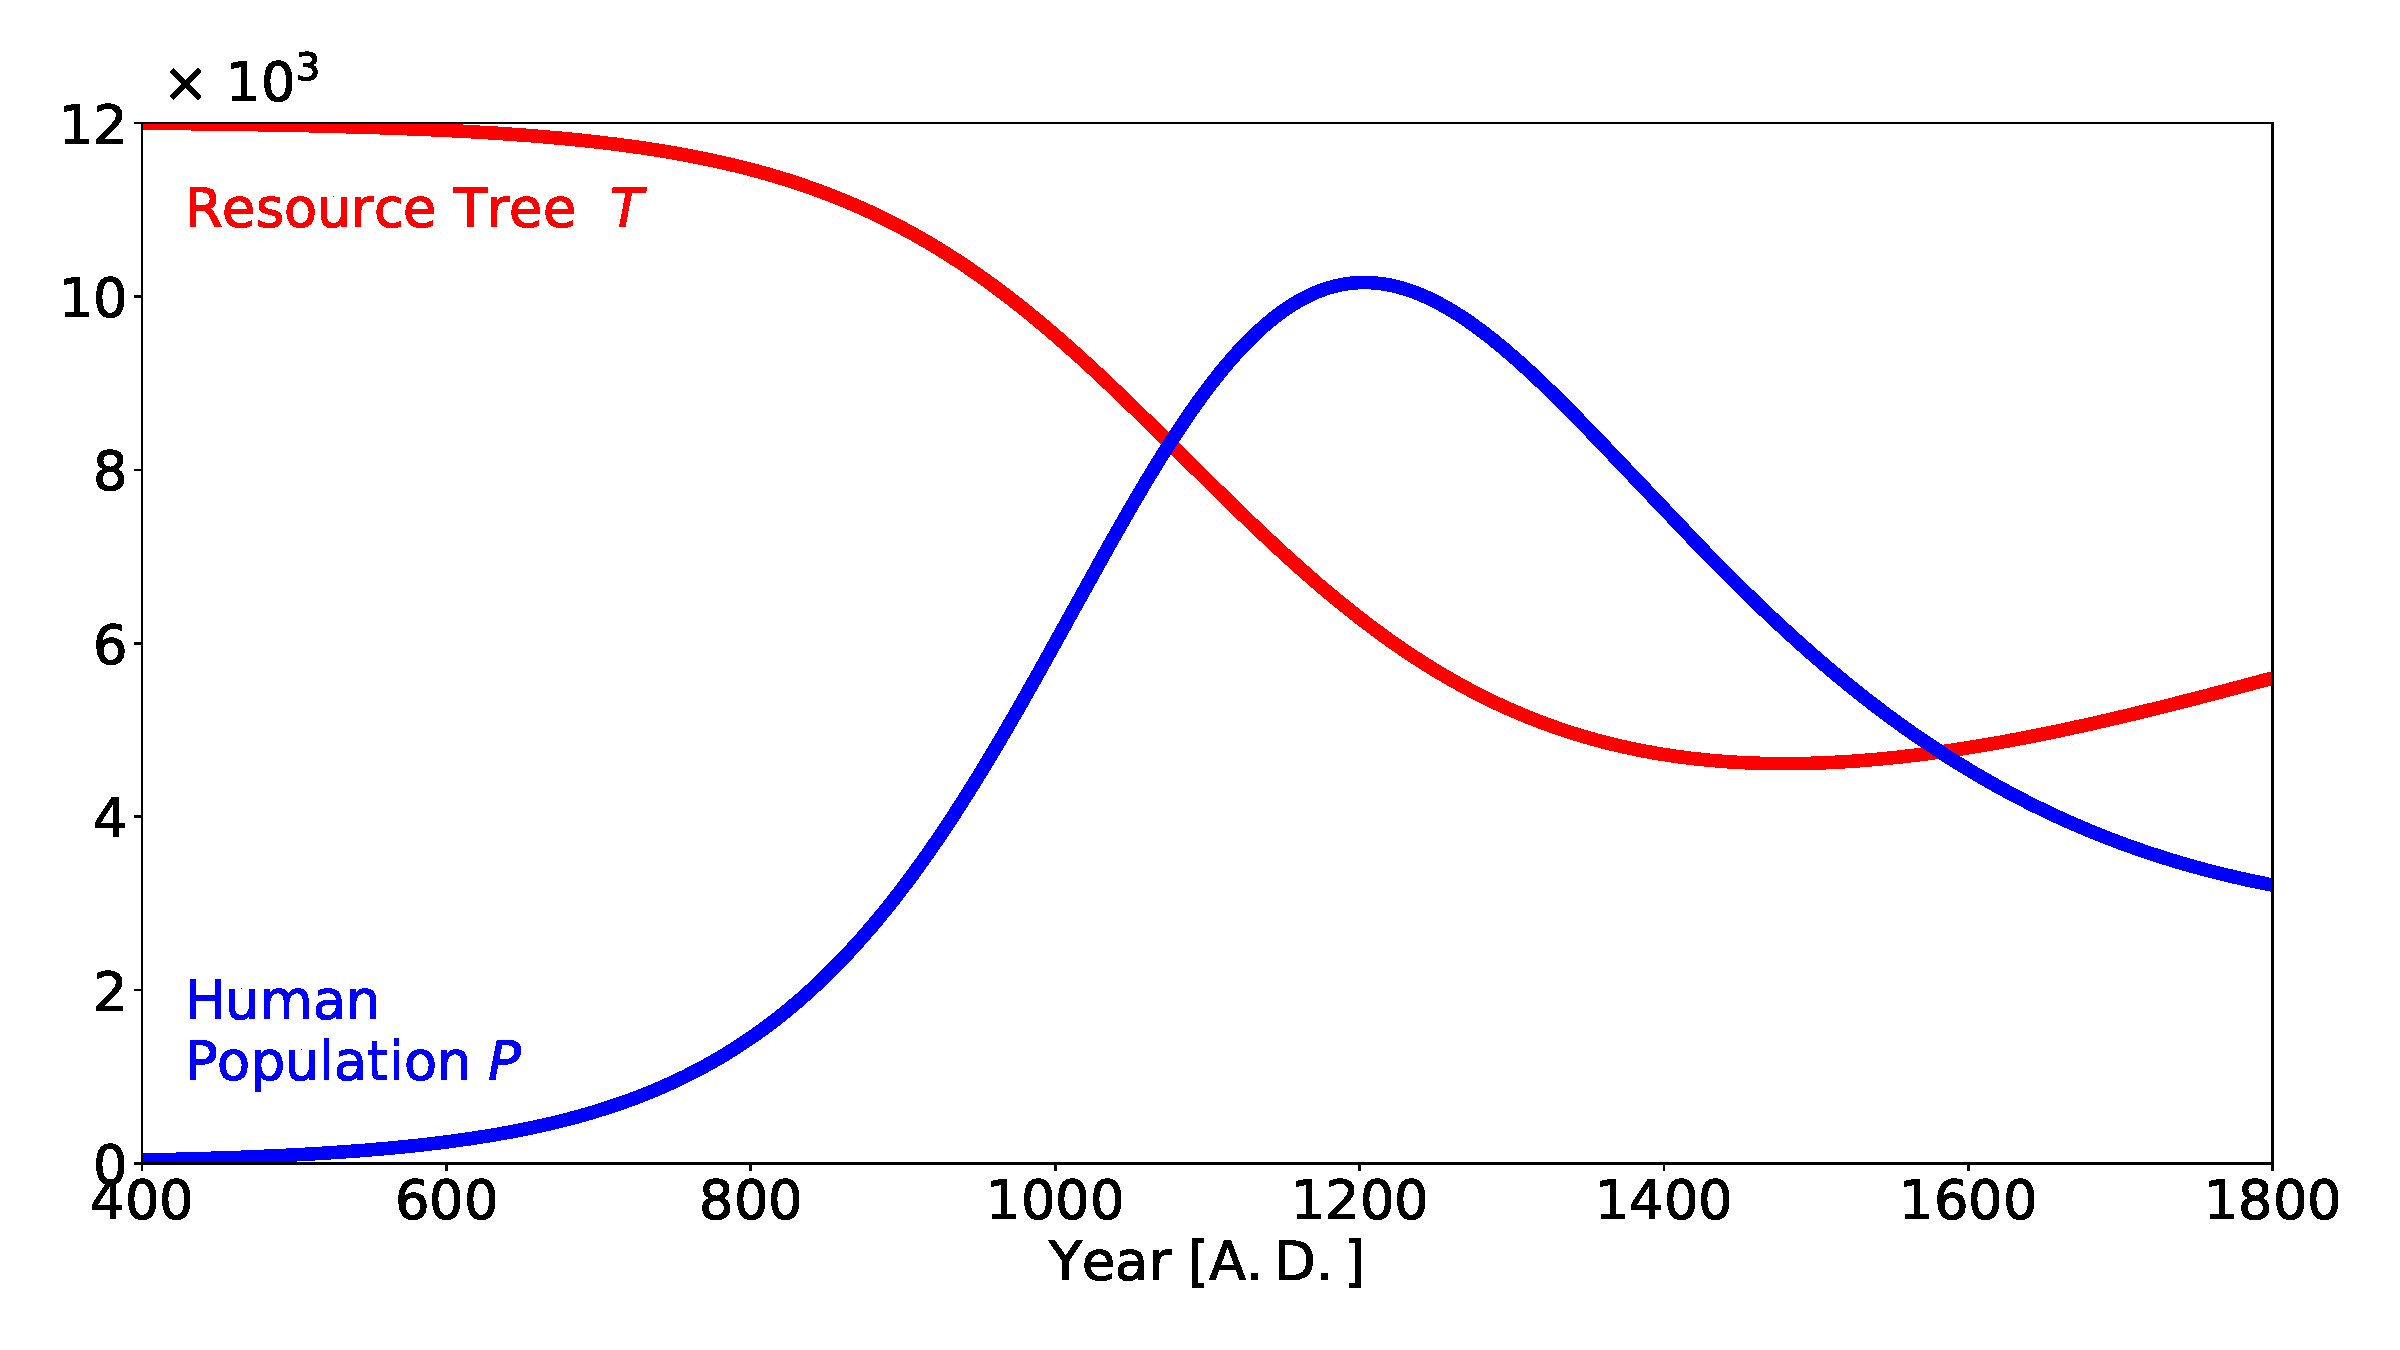
\includegraphics[width=1 \textwidth]{images/Brander1998Model_EI_reduced}
	\caption{Replication of the model in \citet{Brander1998} with parameter setting as in the `Easter Island Base Case' in Figure 3 of the publication. %The dots on the right represent the equilibrium values.
	}
	\label{fig:brander1998eibasecase}
\end{figure}

\paragraph{Extensions of the Basic Model.}
In the last two decades several extensions and adjustments have been added to the first mathematical model by \citet{Brander1998}.
\citet{Reuveny2012} provided an extensive overview of these models.
\citet{Merico2017} additionally summarised gaps and advances within this field of research. 
Here, I point out those models relevant to the word of this thesis.
\citet{dAlessandro2007} separated the single resource into two, one that is inexhaustible and another that is renewable (and irreversibly exhausts if below a certain threshold).
The author found multiple stable states due to this disaggregation of the ecological variable. 
A model by \citet{Good2006} introduced foresight and resource management institutions (either a system of property rights or a social planner).
%to the simple predator-prey harvest in \citet{Brander1998}.
Here, the society's harvest rate is determined by maximising a utility function over a certain time horizon with reasonable discounting (e.g.\ by a social planner, which could be an emergent political hierarchy).
However, the authors found that even with optimal institutions in place, a collapse of the Rapa Nui population is inevitable.
\citet{Basener2008} added another variable to the model next to tree number and human population size, which accounts for the rat population and their devastating impact on tree regrowth as previously found by \citet{Hunt2007}. 
This model was then further extended by a spatial component \citep{Basener2011}. 
A number of homogeneous, one-dimensional cells was defined and diffusion of rats and humans allowed between adjacent cells. 
The authors found that simply changing the mobility of rats can qualitatively alter the dynamics of the human population size.
While this representation is extremely simplified and the diffusion process is unintuitive for human settlement pattern of a small island, this is the only model on Easter Island including a physical space.
Finally, in a recent analysis, \citet{Brandt2015} extended the model of trees, rats, and humans by \citet{Basener2008} with a disease spreading model.
They found that the model can obtain any of the proposed narratives (ecocide, genocide or the slow-demise) through variation of only a few parameters in a reasonable range.
All these models build on the assumptions considered in the macroscopic ODE model by \citet{Brander1998}.


\paragraph{Shortcomings of Macroscopic ODE Models.}
Despite the extensive body of research presented by the numerous macroscopic system models on Easter Island, the dispute between different narratives could not be solved.
The ODE based models, the main tool for Easter Island modelling, typically either showed the same (inherent) boom and bust cycle or showed shortcomings in that different choices of parametrisation (within the uncertainties of the sparse archaeological data) consistently produced contrasting results \citep{Merico2017}.
%ODE-type modelling can only have limited significance.
Next to the uncertainties in the available data to support the assumptions, many shortcomings of these models are inherent problems of macroscopic system modelling.
This includes in particular the missing spatial, microscopic constraints, heterogeneity in the human population, the stochastic nature of the spatial and temporal environment, co-evolving behaviour and emergent phenomena.
A microscopic, agent-based model addresses many of these issues and, therefore, constitutes a useful alternative to macroscopic ODE model approaches as described in the next Section.
%E.g.\ the model by \citet{Brander1998} assumes open access to the resources which defers intuition since the location of an individual restricts the availability of resources. 
%Other models \citep{Good2006} might include a more complex economic which incorporates restrictions on resource harvest but implemented via a social planner.
%Thus, such dynamics are not co-evolving or emergent but externally established 

%While models like \citet{Good2006} have restrictions on the amount of resources, it require a social planner and it is not so much an emergent restriction of the population dyanmics but rather a institution.

\FloatBarrier
\section{Agent-Based Modelling (ABM) of Human-Resource Interactions -- Overview, Motivation and Previous Approaches}
%\begin{itemize}
%\item What is Agent Based Modelling
%\item The basic structure of an ABM in human resource interactions: Agents in environment, Update all agents asynchronously, update environment. Within each update agents change their local environment and their behaviour/properties are in turn influenced by the local environment. 
%\item It breaks with ODE-type of modeling because it enables: 
%\begin{itemize}
%	\item spatially explicit modelling,
%	\item  emergent global behaviour from local rules, 
%	\item computational irreducibility of agent behaviour in terms of crisis. 
%	\item Non-ergodic relation between agents and their environment.
%	\item Stochasticity is natural in the decision making process, due to an agent's imperfect knowledge of the global sitution
%\end{itemize}
%\item ABM in ancient historical population dynamics: Maya \citep{Heckbert2013} and Anasazi \citep{Axtell2002}
%\item Why ABM could help in Easter Island modelling: \citet{Merico2017}.
%\item Structure of this thesis.
%\end{itemize}

\paragraph{Overview of ABM.}
Agent-Based Modelling (ABM) is now a common tool at the centre between cognitive psychology, game theory, and complexity science \citep{Bousquet2004} with roots in the field of Artificial Intelligence.
In Agent-Based Models (ABMs) a system is grown bottom-up from its constituent units.
Hence, an ABM focuses on the microscopic rather than the macroscopic aspects of a system.
The model simulates a number of discrete agents (e.g.\ humans), often situated in an environment, with specific traits.
Agents (and the environment) are updated asynchronously at certain time steps over the simulated period.
In each update, a single agent interacts with the environment and other agents according to a set of rules or heuristics.
These rules are usually heterogeneous, non-linear (e.g.\ discontinuous or discrete), stochastic, time-dependent and adaptive and might be memory- and path-dependent \citep{Bonabeau2002}.
In the case of a spatial model, rules and behaviour additionally depend on the explicit location of an agent in the environment.
Usually, agents make individual decisions, based on perceptions of their local surroundings and their internal state, and thereafter act independently and autonomously.
With this microscopic setup, overall macroscopic dynamics of the system are obtained.
Aggregate system variables can then be interpreted both as outcomes of and as contexts for the agents' decisions and actions \citep{Kohler2000}.
As described in \citet{Bousquet2004}, the mathematical analysis of an ABM, however, is not straight-forward, unless the model is extremely simplified and general.
In fact, validation of an ABM is classically done by simply running simulations (enabled by the rise of computational power in the recent decades), obtaining aggregated system variables and comparing them with observations or testing them for plausibility.

%The field of Agent Based Modelling originally comes from Artificial Intelligence study. 
% WHERE FROM 
% INFORMATICS, EXAMPLES, ...


%These are updated asynchronously in certain timesteps over the simulation period. 
%In each update, a single agent interacts with the environment and other agents and adapts its own features.
%Usually, agents act independently and based on individual decision making by evaluating their state at the current time.
%Aggregate variables of all agents are then a combination of context as well as outcome \citep{Kohler2000}.



\paragraph{Advantages with respect to ODE Models.}
ABMs are applied to study complex systems, i.e.\ systems consisting of multiple components interacting with each other and, thereby, creating feedback loops and non-linearities, because of which the behaviour of the system can not be easily inferred from the input of the model.
%In many complex systems, 
In such systems, ABMs are typically advantageous over macroscopic system models by accounting for the following system properties \citep{Bookstaber2019}:
\begin{itemize}
	\item Emergent phenomena from local, heterogeneous behaviour of the agents,
	\item Computational irreducibility of agent behaviour (e.g.\ in the decision making in times of crisis),
	\item Non-ergodicity of relations between agents and their environment, i.e.\ conditions and rules of behaviour co-evolve with the agent and environment \citep{Kohler2000},
	\item Stochasticity in actions and decision making processes, due to imperfect knowledge or uncertainty of the agents. 
\end{itemize}
Additionally, ABMs allow for a very natural and flexible implementation\footnote{Compare for example with the unintuitive diffusion process in the ODE model by \citet{Basener2011}.} of an explicit space dependency of rules and a spatially heterogeneous environment.
%In ODE models, space dependency is typically implemented via non-intuitive, complex diffusion processes (compare to the model by \citet{Basener2011}).
%In such systems, ABMs are often the most natural and flexible way of describing a system.
%An ABM is especially relevant if a system exhibits emergent phenomena, i.e.\ individual behaviour according to rules cummulates in complex macroscopic patterns.
In particular, if a system exhibits emergent phenomena, crucial information is lost when the heterogeneity of agents is reduced to one representative agent by averaging, as done in macroscopic ODE models \citep{Bonabeau2002}.
Instead, an ABM generates emergence from bottom-up by accounting for non-linear feedbacks due to heterogeneous agents and stochasticity. % e.g.\ connected to uncertainty in the decision making process.

%Furthermore stochastic, discrete processes as in an ABM lead to complex responses of the model outcome, that can not be simply 
% while an ABM gives rise to non-linear feedbacks of fluctuations e.g.\ in the case of uncertainty.
%In such cases, simple averaging and expressing processes by a representative behaviour, as applied in macroscopic system modelling, does not capture emergent phenomena.
%However, an ABM gives rise to non-linear feedbacks from heterogeneous, fluctuating agents e.g.\ in the face of uncertainty and imperfect knowledge in decision making.


\paragraph{Application in Socio-Ecological Systems.}
ABMs have traditionally been applied to problems connected to flows, markets, organisations, or diffusion \citep{Bonabeau2002}.
Typical applications include e.g.\ traffic jams, ant colonies or swarm behaviour of fish and bird flocks.
However, ABMs are also a common approach for socio-ecological systems \citep{Muller-Hansen2017}.
Such a system comprises complex co-evolution of the heterogeneous humans and environment, which interact with each other in non-linear, adaptive ways on multiple time and spatial scales, making it suitable for the application of ABMs \citep{Bousquet2004}.

%The population dynamics of ancient societies 
%, as agents in such a system usually also act heterogeneously and dependent on local space.
%Here, social structure such as the emergence of political organisations in the agent-agent interactions are at the heart of Agent-Based models.
%As agents in ecological systems usually act heterogeneously and strongly dependent on their local environment or neighbourhood, the usage of ABM with an explicit space dependency is suitable \citet{Bousquet2004}.
% motivates the use of ABM in ecological modeling with the local response 

%According to \citet{Bousquet} ABMs in the ecosystem context can be applied to either create scenarios showing `what might be rather than what is' to understand a system or to produce reality-like scenarios in order to test `what if' questions.

%The disadvantage of ABM is that there's no mathematical proof.Bousquet2004.

\paragraph{Application for Ancient Civilisations.}
Agent-Based Modelling has also been applied to study the history of two ancient civilisations.
\citet{Axtell2002} and \citet{Janssen2009}, used an ABM to reproduce the spatio-temporal history of the Anasazi society in a valley in Arizona, US, and its disappearance around $1300\, {\rm A.D.}$. 
Agents in the model represent households with various heterogeneous attributes that interact with the environment via farming. 
The environment is determined from an extensive data record of harvest yield potential in the valley over time and the Agent-Environment interaction is based on this yield and a set of anthropologically plausible rules.
Agents choose a location for a farm depending on the maximum potential yield in a certain distance to water and for the nearest possible settlement with access to water. 
The harvest success determines the fertility and, thus, the dynamics of agent numbers and overall population in the valley.
\citet{Heckbert2013} developed an ABM for the Maya civilisation resulting in a `somewhat analogous' reproduction of the spatial pattern and timeline.
The agents in this model generate a certain amount of agricultural yield on a discretised map based on a benefit-cost assessment. 
They are further connected in clustered, adaptive trade networks, from which they benefit.
Both of these approaches by \citet{Axtell2002} and \citet{Heckbert2013} attempted to explain the spatio-temporal history of an ancient civilisation by developing an Agent-Based Model with anthropological rules and a biologically, geographically explicit environment on a discretised map.


\paragraph{Motivation for Applying an ABM on Easter Island.}
This thesis presents a similar Agent-Based modelling approach for the history of Easter Island.
I have discussed many aspects and advantages of ABM, which apply in socio-ecological systems, and for modelling ancient societies (and Easter Island in particular).
Similar to the valley of the Anasazi, Easter Island is a small, confined space with distinct geographical and biological features with heterogeneous agricultural suitability.
\citet{Merico2017} further argues for the use of an ABM for Easter Island to overcome the shortcomings of ODE models and limits of the available archaeological and palynological data.
The main features of the ABM presented here, thus, include a spatially explicit environment, locally confined agent-environment interaction, a simple adaptation strategy of agents to environmental degradation and individual, stochastic moving decisions by agents.



% !TEX root=frame_thesis.tex
\chapter{Development of an Agent-Based Model for Easter Island of Human Resource Interaction}\label{chapter:Methods}
\FloatBarrier
\section{Model Overview}
%Topic: General overview of ABM
%Main Idea: Human agents interact with local Environment
I present an Agent-Based Model (ABM) that simulates the spatial and temporal history of household agents on Easter Island and their interactions with the natural environment. 
The environment is encoded on a 2D discretised map with heterogeneous geographic and biological features.
Agents rely both on a limited, non- or slowly renewable resource, the palm trees, and a limited, renewable resource, farming produce from arable land (in particular, sweet potatoes). 
They obtain these resources by cutting trees and farming viable sites in their near surroundings, thereby changing their local environment.
Consequently, the household's population growth or decline depends on the success of this resource acquisition. 
Furthermore, resource availability and other geographic indicators determine the settlement behaviour of the agents.
The interaction with the natural environment, thus, constrains the settlement patterns as well as the population dynamics of the overall Easter Island society.

%Topic: Time and Update Order
The model assumes yearly updates of the characteristic variables of each household agent and the environment throughout the simulated time period.
The simulation starts with the arrival of the first settlers at Anakena Beach in
\begin{equation}
t_\text{arrival} = 800\, {\rm A.D.}\ ,
\end{equation}
following \citet{Bahn2017}\footnote{Other arrival dates are discussed in Section \ref{sec:PopGrowth}.}.
The initial population is assumed to be $\mathbf{pop}_{\rm arrival} = 40$ individuals (as in \citet{Brander1998}, and similar to \citet{Brandt2015}) spread on $2$ households, that both settle close to Anakena Beach.
After each time step, $\Delta t=1\,{\rm yr}$, all agents are updated and interact with their local environment sequentially in a randomised order. 
New household agents can appear throughout the simulation following reproduction and splitting of existing agents. 
Following the alteration of the environment by all agents, the environment's state variables are updated (e.g.\ potential regeneration, or soil degradation) once per year (natural update).
The simulation ends in $1900\, {\rm A.D.}$ with the arrival of frequent European voyages, slave trade and European diseases marking the end of the isolated status of the historic Easter Island society .%, since this presumably had a large impact on the society, e.g.\ through the introduction of diseases wiping out a large fraction of the Easter Island population in the 19th century.% \todo{cite Bahn2017}.
%\begin{algorithm}
%	\caption{General Structure}
%	\STATE $t=t_{\rm arrival}$
%	\INITIALISE $N_{\rm Agents}(t_{\rm arrival}) = 2$ with $pop_{\rm i}(t_{\rm arrival})=20$ $\forall i \in N_{\rm Agents}$ and $(x_{\rm i}, y_{\rm i}) (t_{\rm arrival})$ close to Anakena Beach
%	\FOR{$t \ \in\  \{t_{\rm arrival}, t_{\rm end}\}$}
%		\STATE IndexList $\leftarrow$ Order all $N_{\rm Agents}(t)$ Agents in a random Order
%		\FOR{for agent $i\ \in \ $ IndexList}
%			\STATE $F_\text{i}(t) \leftarrow F_{\rm i}(t-1)$
%			\STATE $T_\text{i}(t) \leftarrow 0$
%			\STATE $F_\text{ Req, i}(t) \leftarrow (1-T_\text{Pref, i}(t)) F_\text{Req, pP} \cdot pop_{\rm i}(t)$
%			\STATE $T_\text{Req, i}(t)$
%			\IF{Agent $i$ is a fisher or can become a fisher ($c_{\rm i}(t) \in C_{\rm A}(c_{\rm Anakena})$ \AND $N_{\rm Fisher}<N_\text{Max Fisher}$)}
%				\STATE Make agent $i$ a fisher
%				\STATE  $F_\text{i}(t) \leftarrow F_\text{ Req, i}(t)$
%			\ELSE[Agent $i$ needs to farm]
%				\FOR{$PI \in \{\text{Well-suited, Eroded, Poorly Suited}\}$ }
%				\WHILE{$F_\text{i}(t) < F_\text{ Req, i}(t)$ } \OR {No unoccupied sites in cells $c \in C_{\rm F}(c_{\rm i}(t))$}
%					\STATE Acquire more farming land by \ldots 
%					\STATE \ldots Extending $A_\text{F, i} (t)$ with an unoccupied site in a randomly chosen cell $c\in C_{\rm F}(c_{\rm i}(t))$ with $F_{\rm PI}(c)=PI$
%					\STATE (\ldots if necessary via burning trees to clear the land)
%					\STATE \ldots $F_\text{i}(t) \leftarrow F_{\rm i}(t)+F_\text{PI}(c)$
%				\ENDWHILE
%			\ENDIF
%			\WHILE{$T_\text{i}(t) < T_\text{Req, i}(t)$}
%				\STATE Choose $c$ with $T(c,t) >0 $ from all $c\in C_{\rm T}(c_{\rm i}(t))$
%				\STATE If $c$ exists, $T_\text{i}(t) \leftarrow T_\text{i}(t) $ and $T(c,t) \leftarrow T(c,t) -1 $ 
%			\ENDWHILE
%			\STATE $h_{\rm i}(t)$
%			\STATE $H_{\rm i}(t)$
%			\STATE $pop_{\rm i}(t+1)$
%			\IF{$pop_{\rm i}(t+1) > \mathcal{N}(\TODO, \TODO)$}
%			\STATE Split Agent $j=N_{\rm Agent} +1$ with $pop_{\rm j}=12$ and move agent $j$.
%			\STATE $pop_{\rm i}(t+1) \leftarrow pop_{\rm i}(t+1)-12$ and remove free not needed farmed land
%			\ENDIF
%			\IF{$pop_{\rm i}(t+1) < Min\TODO$}
%			\STATE Remove Agent $i$ and distribute remaining individuals to agents within $C_{\rm M}(c_{\rm i}(t))$
%			\ENDIF
%			\IF{$H_{\rm i}(t)<H_{\rm equ}$}
%			\STATE $(x_{\rm i}, \ y_{\rm i})(t+1) \leftarrow $ Move
%			\ENDIF		
%		\ENDFOR
%		\STATE $F_{\rm PI}(c,t+1) \leftarrow$ Eroded Soil?
%		\STATE $T(c,t)$ 
%	\ENDFOR
%\end{algorithm}

%Topic: I will describe the Model
In Section \ref{sec:CreateMap}, I describe the generation of the 2D discretised map comprising the environment of Easter Island as well as the yearly natural updates. I then focus on the household agents and the update procedure of a single agent:
%This update is separated into several modules: Calculating of the agents' resource requirements, cutting trees, farming, increasing/decreasing population of the agent, and potentially moving the settlement.
This comprises the calculation of agent specific features (Section \ref{sec:agentprops}), the interaction between an agent and the environment (Section \ref{sec:Harvest}), and the consequent response of the agent's properties to the harvest, i.e.\ population growth or decline (Section \ref{sec:APPpopgrowth}) and potential relocation of the agent (Section \ref{sec:Moving}).
Figure \ref{fig:SketchABM} summarises all environmental variables, the agent variables, and their dependencies (except for relocation (described later in Figure \ref{fig:sketchmoving})).

\begin{figure}[H]
	\centering
	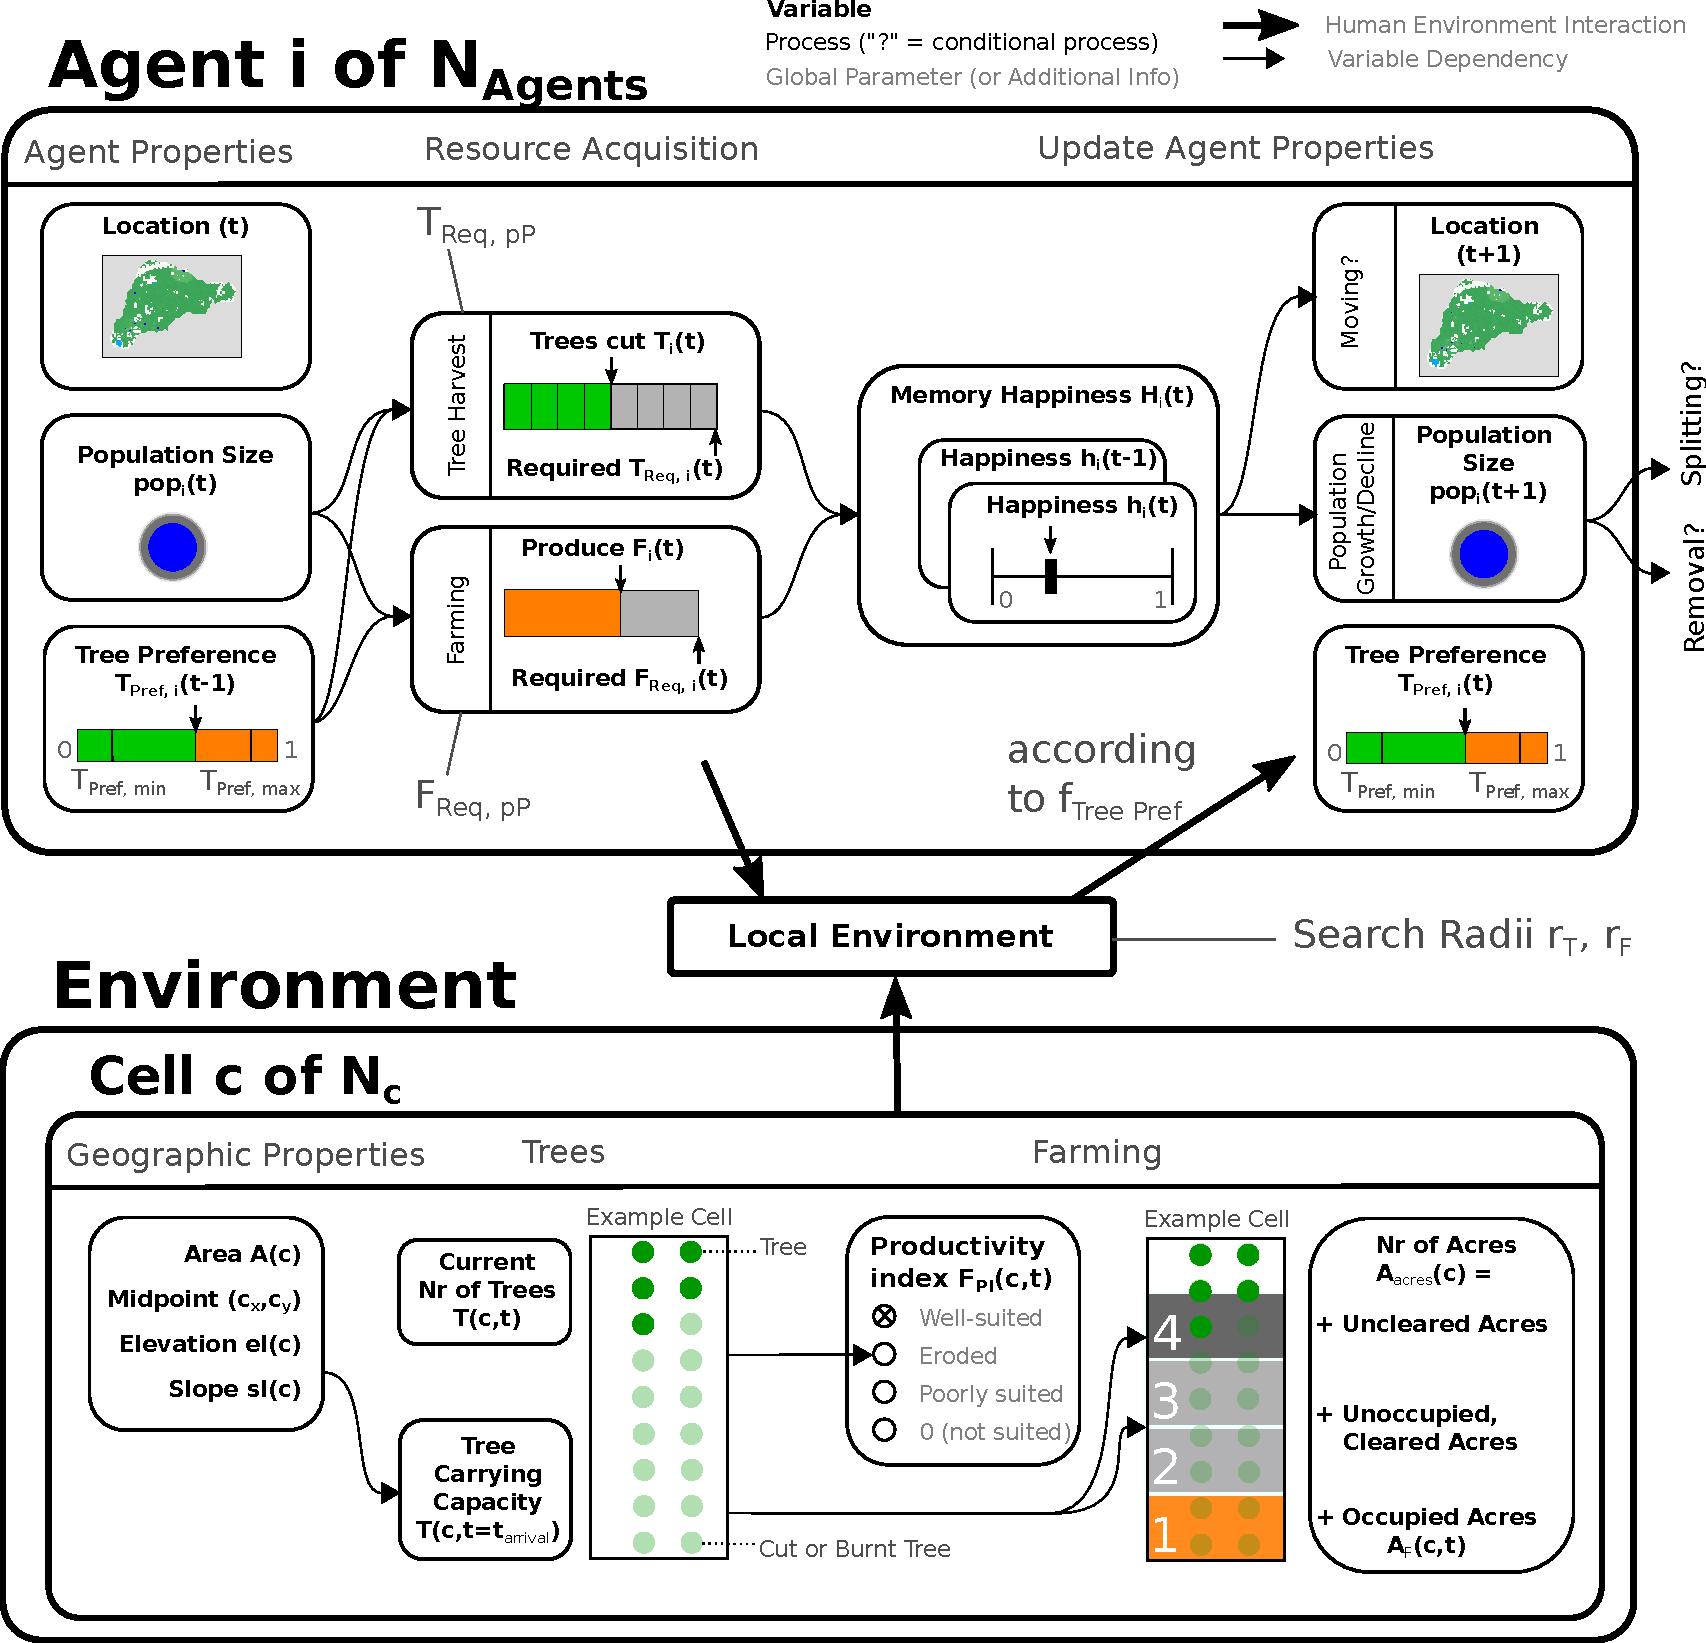
\includegraphics[width=1\textwidth]{images/SketchABM2/sketch.pdf}
	\caption{
		A sketch of an update step of agent $i$ in this ABM, which is described in detail in Chapter \ref{chapter:Methods}.
		The environment consists of $N_\text{c}$ discretised cells, $c$, with certain geographic properties: Area $A(c)$, midpoint $\vec{c}$, terrain elevation $el(c)$, and slope $sl(c)$.  %population density $\frac{pop(C_\text{F}(t)}{r_\text{F}^2\pi}$) (within cells in a circle with radius $r_{\rm F}$, $C_{\rm F}(c)$) 
		A cell has furthermore two `resource stocks'.
		The first resource stock is the number of trees $T(c,t)$, with a maximum of the cell's carrying capacity (and initial state) $T(c,t=t_{\rm arrival})$, which depends on $el(c)$ and $sl(c)$. 
		The second resource stock is the number of arable (i.e.\ cells with a Farming Productivity Index $F_{\rm PI}(c,t)>0$) sites, $A_\text{acres}(c)$, with a basic unit of $1\, {\rm acre}$, consisting of uncleared, cleared but unoccupied and occupied sites ($\mathbf{A}_\text{F}(c,t)$ in acres).
		Agent $i$ represents a household with a population size $pop_\text{i}(t)$, a settlement location $(x_\text{i},\, y_\text{i})(t)$ (corresponding cell $c_\text{i}(t)$), and a tree preference $T_\text{Pref, \, i}(t-1)$, reflecting the state of the local environment in the previous year. From the population size and tree preference (and global, tunable per person resource requirement parameters, $T_{requ, \, pP}$ and  $F_\text{requ, \, pP}$) the corresponding requirements for tree cutting, $T_\text{Req, \, i}(t)$ and farming, $F_\text{Req, \, i}(t)$, are calculated each year.
		The success of the resource acquisition from the local environment determines the current and memory happiness of the agent, $h_{\rm i}(t)$ and $H_{\rm i}(t)$. %requirements depends on the resource stocks of cells in radii $r_{\rm T}$ for tree harvest and $r_{\rm F}$ for farming. 
		This latter then determines the agent's population dynamics (including potential splitting or dispersion of the agent) and whether or not the agent relocates the settlement (according to a semi-rationale decision making process sketched in Figure \ref{fig:sketchmoving} later).
		Finally, the tree preference, $T_\text{Pref, i}(t)$ is updated reflecting the state of the changed local environment.
	}
	\label{fig:SketchABM}
\end{figure}

\FloatBarrier
\section{A Discretised Map of Easter Island with Geographical and Biological Features}\label{sec:CreateMap}
\paragraph{Map Discretisation}
I create a discretised map dividing the island into a number of small 2D triangular cells with certain geographical features.
First, I define an equidistant grid on Easter Island\footnote{Ranging $18\, {\rm km}$ in latitudinal (from $-27.2050^\circ N$ to $-27.0437^\circ N$) and $24\, {\rm km}$ in longitudinal direction (from  $-109.4650^\circ E$ to 
 $-109.2227^\circ E$)} with a grid size of $\delta_{\rm x} \approx 320\, {\rm m}$ between points in $x$- (i.e.\ $75$ points) and $\delta_{\rm y} \approx 360\, {\rm m}$ in y-direction (i.e.\ $50$ points). 
In principle, the map can be created with any arbitrary resolution, constrained only by the resolution of the underlying geographical data. 
Also other grid types, e.g.\ with adaptive $\delta_{\rm x,y}$ to focus on regions of interest, are compatible with the model. 
While a higher resolution increases detailed geographical representation and reduces discretisation errors, computation time of the presented model scales highly non-linearly (see Section \ref{sec:Moving}).
Hence, a trade-off has to be found between detail or accuracy and computation time.
Next, I create 2D triangular cells from this grid using \textit{matplotlib}\footnote{\citet{matplotlib}}'s Delaunay triangulation package.
A cell $c$ is characterised by its midpoint $\vec{c} = (c_{\rm x},\, c_{\rm y})$. 
Since all cells are Delaunay triangles, their smallest angles are maximised and, hence, the midpoint, $\vec{c}$, provides a reasonable representation of the cell.
%Topic: Define Easter Island
%Using geographical information, the triangles making up Easter Island are selected.
The terrain features, elevation, $el(c)$, and slope, $sl(c)$, of Easter Island are obtained from a publicly available, high resolution elevation map \citep{Jarvis2008CIGAR} via the Google Earth Engine interface\footnote{\citet{gorelick2017google}} and evaluated at the corresponding midpoint $\vec{c}$.
All cells located on the ocean (i.e.\ $c$ with $el(c)=0$) are masked out and discarded.
The cells corresponding to the island's three small crater lakes are also identified.
The remaining cells constitute the landmass of the discretised island, which can later be settled, deforested or farmed by the agents. 
With the resolution given above, $N_{\rm c} = 2768$ cells remain with an area of roughly $A(c)= 0.06 \, {\rm km^2} = 14.2 \, {\rm acre}$.
The area of the obtained discretised Easter Island map is $A=159.2\, {\rm km^2}$, ($163.6\, {\rm km^2}$ in reality) providing a detailed, cellular representation of geographical features (location $\vec{c}$, area $A(c)$, elevation $el(c)$, and slope $sl(c)$).

%There are three -- or two in periods of major droughts (see \citet{Rull2020}) -- permanent crater lakes on Easter Island, providing the major freshwater sources for the prehistoric Easter Island population, as discussed later in Section \ref{sec:Moving}.
%The corresponding cells are calculated from the locations and radii of these lakes. 
%This procedure gives a detailed, discretised representation via triangular cells with geographical features of Easter Island. 
 
%Archaeological records indicate that crater lakes could have dried out during major drought periods.
%In particular the drying of Rano Raraku in the East of Easter Island during the Medieval Climate Anomaly ($500-1200 \, \rm{A.D.}$) and during the Little Ice Age ($1570-1720\, \rm{A.D.}$) \citep{Rull2020} and the consequences have been a reoccuring theme of scientific debate (e.g.\ \citet{Cauwe2011}). 
%Such drought events can be simulated by removing each of the lakes for some period of time from the map.

\paragraph{Trees}
%Next to purely geographical, each cell has characteristic biological features, trees and .% next to the geographic specification before. 
Each cell $c$ on the discretised map contains a number of trees, denoted as $T(c,t)$ (or tree density $T(c,t)/A(c)$).
%While the assumption of constant climatic conditions throughout Easter Island's history has been challenged recently \citep{Rull2020}, I only consider anthropogenic deforestation $T(c,t)$.
The island's forest system is assumed to be in equilibrium (c.f.\ \citet{Brander1998}) at the time of the arrival of the first settlers, $t_\text{arrival}$ and, thus, $T(c,t=t_\text{arrival})$ is the constant carrying capacity of palm trees for each cell $c$ on the island. 
There is is still some uncertainty about the total number and spatial patterns of palm trees at $t=t_\text{arrival}$.
\citet{Mieth2015} estimate a total of $16\cdot 10^6$ trees covering $80\%$ of the island from observed root casts in the soil, whereas e.g.\ \citet{Brandt2015} initialise the model with a conservative estimate of $8\cdot 10^6$ trees. 
Most studies assume an island wide, dense distribution of the palm trees. 
E.g.\ \citet{Bahn2017} state that soil sufficient for tree growth is present `almost everywhere on the island, apart from the steepest parts of the cliffs and the youngest lava surfaces' (i.e.\ the highest elevations of Mount Terevaka). 
However, \citet{Rull2020} also investigates the possibility of variable, mosaic vegetation patterns with high densities of trees around the lakes and the coastal areas.
%As mentioned in the introduction \TODO, there's no comprehensive record of tree patterns. While some \todo{cite Rull?} archaeologsits state that the majority ($80\%$ of the island) was densley forrested \todo{cite}. 
The model presented here can incorporate any pattern of pre-arrival tree density. 
For the results in this thesis, I assume 
%by two terrain-dependent tree density levels: (1) `normal density' for low elevation $el(c)<250\, \rm{m}$ and slope $sl(c)<5^\circ$, (2) `half density' for moderately high elevations $250\, \rm{m}el(c)<430\, \rm{m}$ (elevation of Lake Rano Aroi) and slope $5^\circ < sl(c) < 9^\circ$, and (3) `zero density' for cells above these thresholds.
a total\footnote{Bold symbols denote iterations over all cells (or agents) in the thesis.} of 
\begin{equation}
\mathbf{T}(t=t_\text{arrival}) = \sum_{c} \, T(c,t=t_\text{arrival}) =  16 \cdot 10^6
\end{equation} 
trees distributed according to an equal density pattern excluding those cells with very high elevation or slope ($el(c)>450\, {\rm m}$ or $sl(c)>10^\circ$ $\Rightarrow$ $T(c,t) = 0$).
% with uniform probability among all cells with potential for tree growth. 
A resulting map of pre-arrival tree numbers $T(c,t_\text{arrival})$ in cells $c$ extending on $86\%$ of Easter Island is shown in Figure \ref{fig:Map_tree}.

\begin{figure}
	\centering
	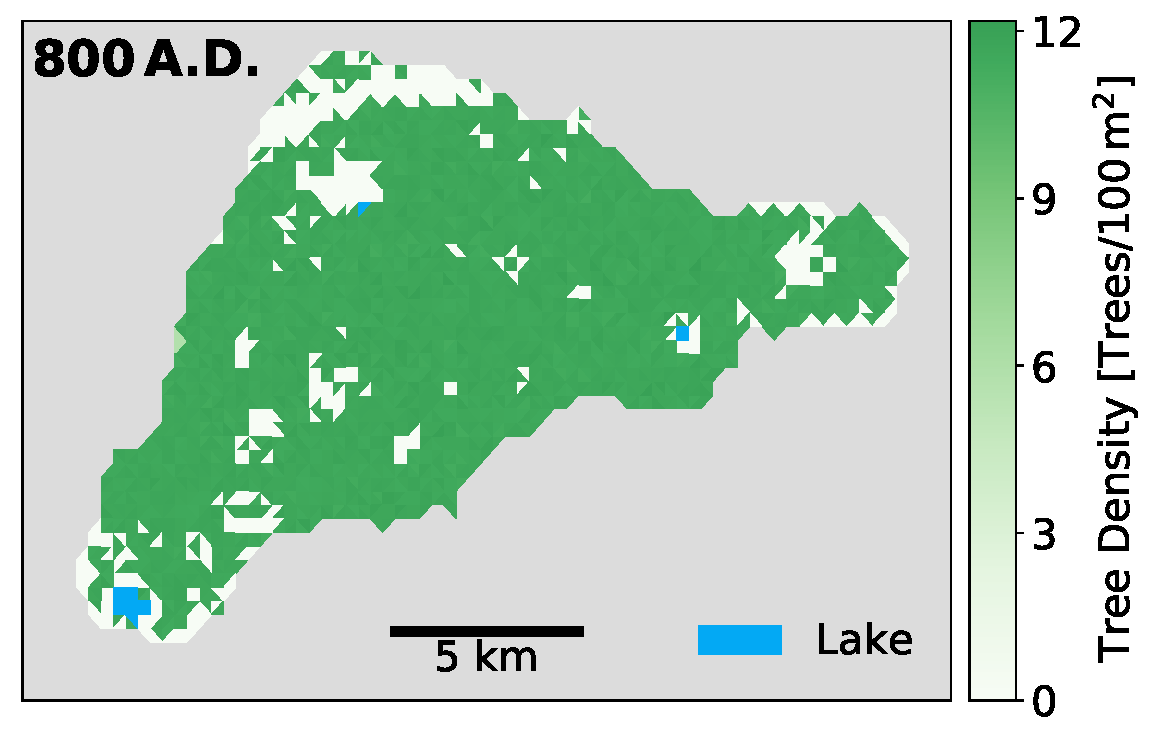
\includegraphics[width=0.7\textwidth]{images/map_carrCap.pdf}
	\caption{The carrying capacity density of trees in each cell $T(c,t_\text{arrival})/A(c)$.}
	\label{fig:Map_tree}
\end{figure}

\paragraph{Tree Regeneration}
Through anthropogenic deforestation, the variable tree number in each cell, $T(c,t)$, declines.
Natural removal (e.g.\ through a changing climate) is not considered in the model.
%As described in the Introduction, the impact of the human deforestation compared to the invasive Polynesian rats on the environmental degradation of the island is debated (e.g.\ \citet{Bahn2017} and \citet{Hunt2007}).
In the literature on Easter Island, there seems to be a consensus between the two major contrasting theories that rats (at least) effectively hindered tree regeneration by gnawing on the palm nuts (e.g.\ \citet{Bahn2017} and \citet{Hunt2007}).
In line with this argument, forest regeneration is not possible in the standard setting of this model.
Trees therefore constitute an entirely non-renewable resource in this scenario. 
However, I also investigate alternative experiments in which the forest can hypothetically regenerate following anthropogenic deforestation.
In this alternative setting, each year, tree numbers $T(c,t)$ in all cells $c$ regrow logistically to their (local) carrying capacity $T(c,t=t_\text{Arrival})$ if there is no farming activity on the specific cells.
The maximum growth rate of this localised logistic tree regeneration is believed to be rather slow and has even been made responsible for the ecological collapse of the island in \citet{Brander1998}.
%Hence, in the alternative experiments, I set the maximum logistic tree regeneration growth rate to
Here, I use (in the alternative scenario)
\begin{equation}
g_{\rm T} = 0.05\, {\rm \frac{1}{yr}} \ .
\end{equation}
based on the estimated maximum tree regrowth rate in \citet{Brandt2015} (between $0.02$ and $0.07\, {\rm \frac{1}{yr}}$ in the absence of rats).
Some cells are deforested entirely in a single update step, which disables logistic regeneration. 
However, with seeds being transported to the empty cell e.g.\ through wind, birds or human activity, forests regrow even from empty spaces.
To incorporate this, a small number of trees `pops up' ($0.5\%$ of the cell's carrying capacity) after a treeless cell has been left barren, i.e.\ without any farming activity, for $10$ consecutive years.
In summary, in this model the tree number in a cell $c$ either (standard setting) does not regenerate at all or (alternative setting) regenerates as
\begin{equation}\label{eq:treeupdate}
T(c,t+1)= \begin{cases}
T(c,t) + T(c,t) \cdot g_{\rm T} \cdot \left(1- \frac{T(c,t)}{T(c,0)}\right) \quad & \forall \ c \text{ with } \mathbf{A}_{\rm F}(c,t)=0 \\
0.005 \cdot T(c,0)  & \forall  \ c \text{ with } T(c,t)=0 \text{ and}\\
& \mathbf{A}_{\rm F}(c,\hat{t})=0 \  \ \forall \  \hat{t} \in \{t-10, \ldots, t\} \\
0 & \text{ else }
\end{cases}
\end{equation}
(neglecting anthropogenic deforestation).
These two scenarios, labelled as without and with forest regeneration, allow for testing of the impact of the Polynesian rats, assuming that they effectively hindered tree regeneration.

\paragraph{Farming Sites}
Next to the resource trees, the environment also provides land for active farming of sweet potatoes\footnote{Sweet Potato was the dominant staple crop on Easter Island (at least in later phases) \citep{Louwagie2006}} as a renewable, second resource (similar to \citet{dAlessandro2007}).
A farming site on arable land has a constant, basic unit area of $1\, {\rm acre}$ on a cell.% and obtain a farming produce according to the cell's farming productivity index.
Hence, if a cell is arable, it provides the possibility for 
\begin{equation}
A_{\rm acres}(c) = \text{Rounded Down }(A(c)[\text{acres}])
\end{equation}
farming sites, which can each be occupied and farmed by an agent.
The number of occupied sites in each cell is denoted as $\mathbf{A}_{\rm F} (c, t)$.
%\begin{equation}\label{eq:occupied}
%\mathbf{A}_{\rm F} (c, t)  = \sum_{j \in N_{\rm Agents}(t)} \, \sum_{a \, \in \, A_\text{F, j}(t)} \, \delta(a=c)
%\end{equation}
%\todo{Occupied Sites Here}
Each farming site provides, if farmed by an agent, a constant output of crop yield each year. 

\paragraph{Farming Productivity Index}
The farming productivity per area, i.e.\ the potential crop yield, is strongly location dependent.
Here, I define a (relative) Farming Productivity Index, $F_\text{PI}(c)$, for each cell $c$ (shown in Figure \ref{fig:Map_agric}). 
While the total potential of farming productivity remains uncertain (as described in the Introduction), some studies used agricultural modelling based on elevation, climate and soil quality data to obtain a more detailed, spatially explicit classification of the farming potential:
%identified arable sites by using data on rain, climate, temperature, elevation and soil quality in agricultural models (e.g.\ \citet{Louwagie2006} and \citet{Puleston2017}).
%A farmed acre yields a produce according to a (relative) Farming Productivity Index, $F_\text{PI}(c)$.
%The absolute productivity of a well-suited acre in units of people it can support is taken from calculations in \citet{Puleston2017} assuming two different Nitrogen fixation scenarios (see in detail later).
%The map of Farming Productivity Indices $F_\text{PI}(c)$ of all cells on Easter Island is shown in Figure \ref{fig:Map_agric}, thus defining where agents have access to farming and how productive farming would have been in this location in the model. 
%Topic: Agriculture Yield
%\paragraph{Studies on the Farming Quality}
%The Easter Island society also cultivated renewable staple crops as an alternative to harvesting the non- or slowly renewable resource, tree\citep{dAlessandro2007}.
%Hence, agents in this model also farm on arable land in a two resource dependency similar to previous models \citep{dAlessandro2007}.
%Agents in this model transfer arable land into farming sites, in particular for sweet potato cultivation, the dominant staple crop on Easter Island (at least in later phases) \citep{Louwagie2006}.
%As described in the Introduction, Easter Island's suitability for farming, especially w.r.t.\ climate and soil, has been subject to excessive debate.
%While the total potential of agricultural productivity remains uncertain, several studies identified arable sites by using data on rain, climate, temperature, elevation and soil quality in agricultural models (e.g.\ \citet{Louwagie2006} and \citet{Puleston2017}).

\citet{Puleston2017} created a map (Figure 4 in the publication) 
indicating regions that meet a certain viability criterion for sweet potato cultivation.
This criterion marks $19\%$ of the island as agriculturally viable, mainly in the lowland, coastal region.
In this model, I denote all cells of the discretised map, which are located in this region `well-suited' and assign a high farming productivity index $F_{\rm PI}|_{\rm well}$.
Additionally, the map includes areas that did not meet the criterion but in which nevertheless small, patchy areas of agricultural structures were identified from satellite images \citet{Puleston2017}. 
Consequently, the yield from these regions must have been low such that the farmers used techniques like labour intensive, large-scale lithic mulching, which mainly increased moisture availability, and efficient crop management, e.g.\ plant spacing and frequent fallowing to obtain yields \citep{Louwagie2006} from these sites.
I call all cells in this region `poorly suited' and assign a low farming productivity index $F_{\rm PI}|_{\rm poor}$.

\citet{Louwagie2006} developed a classification for successful cultivation of several crops based on climate and soil property measurements at a few sites on the island and assigned relative yields to these sites. 
The majority of the measurement sites located at the foots of smaller craters along the arable coasts correspond partly with the well-suited and partly the poorly suited regions\footnote{Comparing roughly Figure 1 of \citet{Louwagie2006} with Figure 4 of \citet{Puleston2017}.}. For most climatic conditions these were classified as mostly `marginally to moderately suitable' for sweet potato cultivation (corresponding to a relative yield of around $55\%$ ($(20-80\%)$) of an optimal farming site) and, especially in wet years, some locations were classified as `highly suitable' (relative yield of $>80\%$).
 One of the studied sites (`Vaitea'), which more clearly coincides with the poorly suited region, was found `not suitable' for farming due to insufficient nutrition availability (relative yield of $0-20\%$) despite archaeological evidence of gardens in this area.
 Following these results roughly, which provide the best estimate available, and naively extrapolating them, I choose
 \begin{eqnarray*}
 	F_\text{PI}|_\text{well} & = 80\% & \text{ for well-suited (highly to moderately suitable)}\\
 	F_\text{PI}|_\text{poor} & = 10\%  & \text{ for poorly suited (not suitable)}\\
 	F_\text{PI}|_\text{non-viable} & = 0\% & \text{ for non-viable sites}
 \end{eqnarray*}
 depending on a cell's classification by \citet{Puleston2017} into well-suited and poorly suited cells.
 Hence, the total resulting arable land area in this model (shown in Figure \ref{fig:Map_agric}) is ca.\ $29\,  {\rm km^2}$ (i.e.\ $18\%$) for well-suited sites and, additionally, $50\, {\rm km^2}$ (i.e.\ $31\%$) for poorly suited sites with low Farming Productivity Index.
%However, only a small, patchy fraction of this `poorly suited' region was actually effectively farmed as estimated by \citet{Puleston2017} by identifying agricultural structures from satellite data. 
% also indicating that there is a strong difference between well-suited sites and those

%\paragraph{Map of Arable Land}
%In order to obtain a spatially explicit differentiation between arable and non-arable land, I use a map created by \citet{Puleston2017} (Figure 4) indicating regions meeting a certain viability criterion for sweet potato cultivation.
%This criterion %is based on an agricultural model of climate data and soil quality and 
%marked $19\%$ of the island as agriculturally viable, mainly in the lowland, coastal region.
%However, widespread systems of gardens were also found in the upland regions classified as non-viable by \citet{Puleston2017}.
%The authors state that these gardens added only a small fraction of actually farmed land to the viable region, though.
%Here, I use three levels of viability for the discretised map: 
%%A cell is either `well-suited' if located in the viable region, `poorly suited' if located in the non-viable region which was nevertheless farmed, or `non-viable' else (cp.\ with \citet{Puleston2017} (Figure 4)).
%
%The difference between well-suited and poorly suited arable land is reflected in the Farming Productivity I
%
%
%The total resulting arable land area in this model (shown in Figure \ref{fig:Map_agric}) is ca.\ $29\,  {\rm km^2}$ (i.e.\ $18\%$) for well-suited sites and, additionally, $50\, {\rm km^2}$ (i.e.\ $31\%$) for poorly suited sites.
%%This fraction of arable land is in line with several different estimates from e.g.\ \TODO \citet{Bahn2017}???
%%. TODO SOMEONE SAID THAT 50\% of the land was cultivated?
%
%\paragraph{Farming Productivity Indices}
%I distinguish well-suited from poorly suited cells by assigning different dryland Farming Productivity Indices, $F_\text{PI}(c)$, to associated cells.
%\citet{Louwagie2006} developed a classification for successful cultivation of several crops based on climate and soil property measurements at a few sites on the island and assigned classes of relative yields to them. 
%One of the studied sites (Vaitea), which coincides with the poorly suited region in \citet{Puleston2017}\footnote{Compare Figure 1 of \citet{Louwagie2006} with Figure 4 of \citet{Puleston2017}.}, was found not suitable for farming due to insufficient nutrition availability (with a relative yield of $0-20\%$ compared to an optimal site) despite archaeological evidence of gardens in this area.
%To enhance yields, the islanders used techniques like labour intensive, large-scale lithic mulching, which mainly increased moisture availability, and efficient crop management, e.g.\ plant spacing and frequent fallowing \citep{Louwagie2006}.
%The per area productivity, however, remains low even with these techniques in place with nutrient availability being the main constraint as also implied by the analysis in \citet{Puleston2017}.
%The other sites in \citet{Louwagie2006} located at the foots of smaller craters along the arable coasts, were classified as mostly `marginally to moderately suitable' for sweet potato cultivation for most climatic conditions with some locations showing `high suitability' (relative yield $>80\%$) especially in wet years. 
%These sites are mainly located in the well-suited or poorly suited regions of the map in \citet{Puleston2017}.
%Hence, following roughly the classification by \citet{Louwagie2006}, a Farming Productivity Indices, $F_\text{PI}(c)$ is assigned to each cell (and its corresponding sites)
%\begin{eqnarray*}
%	F_\text{PI}|_\text{well} & = 80\% & \text{ for well-suited (highly to moderately suitable)}\\
%	F_\text{PI}|_\text{poor} & = 10\%  & \text{ for poorly suited (not suitable)}\\
%	F_\text{PI}|_\text{non-viable} & = 0\% & \text{ for non-viable sites}
%\end{eqnarray*}
%depending on its classification by \citet{Puleston2017} into well-suited and poorly suited cells.

\paragraph{Erosion}
Soil erosion through radical deforestation and heavy rainfalls degraded the farming productivity of the island especially in the later phase (e.g.\ \citet{Brander1998}, \citet{Mieth2005}, \citet{Bahn2017}, \ldots).
As trees are removed from a region, rain can wash away nutrient-rich soil and reveal less fertile ground with reduced relative yield \citet{Mieth2005}.
In the model, I assume that, if a well-suited cell is entirely deforested, the land erodes and, thus, the cell's $F_\text{PI}(c)$ reduces to 
\begin{equation}
F_\text{PI}|_\text{eroded}=50\% \quad \text{for well-suited cells with } T(c,t)=0 \ .
\end{equation}
This soil degradation is reverted as soon as trees pop back up (i.e.\ if the cell has been kept barren (without farming) for $10$ years as described in equation \ref{eq:treeupdate}).


\begin{figure}
	\centering
	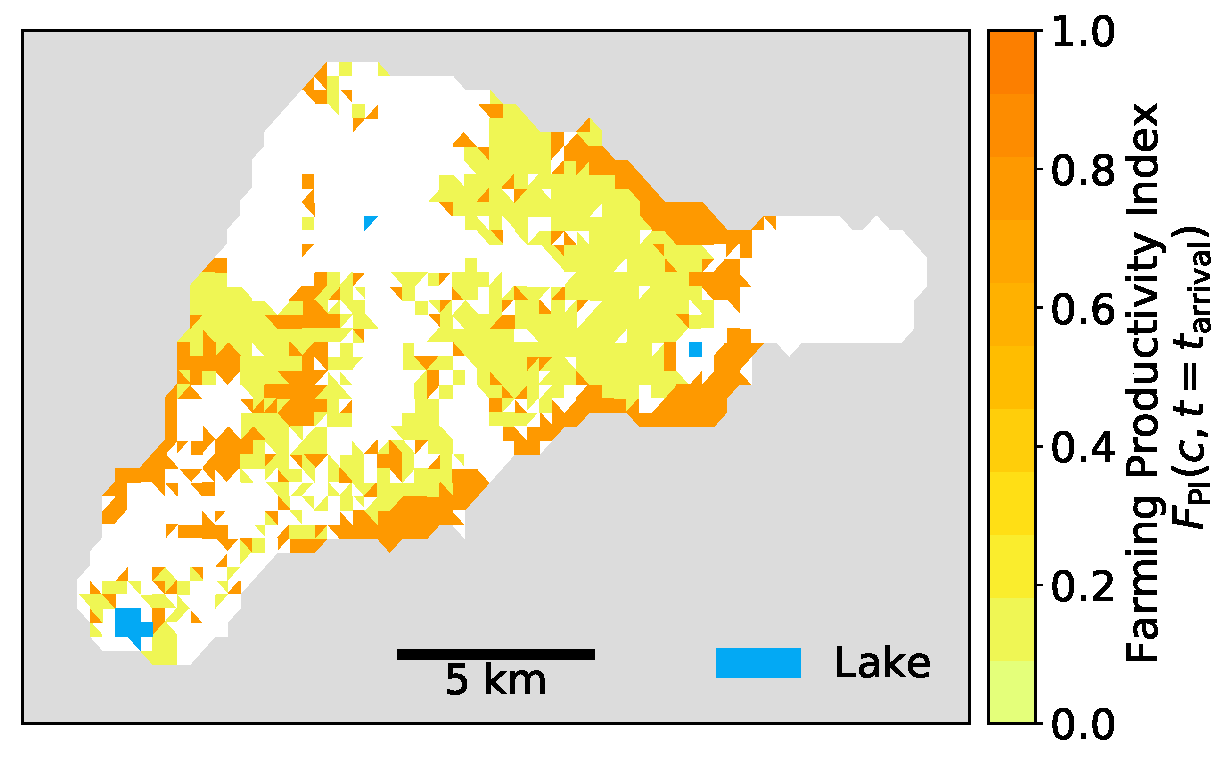
\includegraphics[width=\textwidth]{images/Plot_F_PI_c.pdf}
	\caption{A map of the (sweet potato) Farming Productivity Indices, $F_\text{PI}(c)$, in each cell of the discretised map of Easter Island. The model makes use of the map of \citet{Puleston2017} classifying arable land into viable areas (here `well-suited sites'), non-viable but nevertheless partially farmed (here `poorly suited sites'), and non-viable sites derived from an agricultural model of climate and soil quality. 
	This classification is combined with measurements of land suitability in several sites \citep{Louwagie2006} giving rise to a simple, spatially explicit map of farming potential parametrised by the Farming Productivity Index $F_\text{PI}(c)$.}
	%The Farming Productivity Indices in areas where gardening was observed but that did not meet the agricultural potential of \citet{Puleston2017}'s criterion is $10\%$ in line with the result of a model of agricultural yield from measurments in one such site by \citet{Louwagie2006}.}
	\label{fig:Map_agric}
\end{figure}


%\section{Agent Properties and Agent-Environment Interaction}\label{sec:AgentUpdate}
% Topic: Agents Households with properties
\FloatBarrier
\section{Human Agents and their Features}\label{sec:agentprops}
\paragraph{Basic Variables}
The ABM consists of a variable number of agents, $N_{\rm Agents}(t)$, which represent households, situated on the discretised map derived in Section \ref{sec:CreateMap}.
An agent with index $i$ has several features describing its state at time $t$:
The settlement is located at 
\begin{equation}
	\vec{x_{\rm i}}(t) = (x_{\rm i},\, y_{\rm i})(t)
\end{equation}
 on the discretised map and, hence, associated with one specific cell $c_{\rm i}(t)$.
 The agent's population size, i.e.\ the number of individuals in the household, 
 \begin{equation}pop_{\rm i}(t) \end{equation}
typically ranges from $12$ to ca.\ $42$. % ranging from $6$ to $42$ .
Macroscopic island-wide aggregate variables, like the population size, are simply obtained by summation over all agents, which I denote with bold symbols in the thesis (equivalent to summation over cells). 
%Iterations over all agents (or cells of the map for the corresponding variables) are denoted via bold symbols in all equations in this thesis.

\paragraph{Resource Search Radii}
Agents have access to two different types of resources, trees (and consequent derivates) and farming produce, by interacting with their local environment defined by fixed resource search radii around the agents.
%An agent $i$ harvests these resources from cells with midpoints
% $\vec{\tilde{c}}$ located within fixed radii of the agent's settlement:
Hence, the local environment of agent $i$ is defined as:
\begin{equation} \label{eq:Circle_T}
C_{T}(c_{\rm i}(t)) = \{ \tilde{c}\ | \   | |  \vec{\tilde{c}} - \vec{x_{\rm i}}(t) | |  \leq r_{\rm T} \} 
\end{equation}
for the resource tree with search radius $r_{\rm T} =2\, {\rm km}$ and 
\begin{equation} \label{eq:Circle_F}
C_{F}(c_{\rm i}(t)) = \{ \tilde{c}\ | \   | |  \vec{\tilde{c}} - \vec{x_{\rm i}}(t) | |  \leq r_{F} \}
\end{equation}
for occupying farming sites with radius $r_{\rm F} = 1\, {\rm km}$.

\paragraph{Tree Preference}
The agent's total required resource uptake is split between tree cutting and farming yield, given by a trait parameter, the tree preference $T_\text{Pref, i}(t)$ for agent $i$ at time $t$, which reflects the state of the local environment.
%Changes in the tree preference are an adaption of the agent's harvest behaviour to changes in its local environment.
In the first phase of settling on the island, the civilisation mainly lived off the island's abundant natural resources (here trees) \citet{Bahn2017}.
However, over time, the economy `switched from predominantly hunter-gatherer to a dryland farming society' \citep{Louwagie2006}.
%In the model, this behavioural shift is expressed as a decrease in the variable tree preference parameter, $T_\text{Pref, i}(t)$ of each agent over time.
The tree preference trait, $T_\text{Pref, i}(t)$, in this model is designed such that agent's adjust their harvest behaviour for next year given the current state of the local environment (in particular the level of deforestation).
%Changes in the tree preference are an adaption of the agent's harvest behaviour for next year to changes of the state of its local environment (in particular the level of deforestation).
%It is an adaptive trait reflecting the local state of the environment around an agent, in particular the local abundance of trees. %(i.e.\ trees $T(c,t)$ of cells within $C_{\rm T}(c_\text{i}(t)$).
Hence, as trees are removed from an agent's local environment and more arable land is cleared freeing up space for agriculture, the agent's tree preferences decrease and its farming requirement increases, accordingly.
%This tree preference indicates the value of tree harvest over agricultural production and, hence, increases the need for one over the other in order to fill the resource requirements.
%The tree preference is high in the initial state, but decreases as trees become scarce and more land is available for cultivation of crops.
%Hence, $TPref_{\rm i}(t)$ responds to some degree to the local environment of the agent.
%In this model, $T_\text{Pref, i}(t)$ depends on the local, relative change of tree density within the tree search radius $r_{\rm T}$ with respect to the initial state at $t=t_\text{arrival}$, i.e.:
In this model, $T_\text{Pref, i}(t)$ depends on the relative change of tree density with respect to the initial state at $t=t_\text{arrival}$ in the local environment:
\begin{equation}\label{eq:TPref}
T_\text{Pref, i}(t) = f_\text{Tree Pref}\left( \, \frac{\sum_{\tilde{c} \in C_{T}(c_{\rm i}(t)) } \, T(\tilde{c}, t)}{\sum_{\tilde{c} \in C_{T}(c_{\rm i}(t))} \, T(\tilde{c}, t_\text{arrival}) } \, \right)
\end{equation}
The shape of the function $f_\text{Tree Pref}$ is an indicator of the adaption strategy of the economy/society to environmental change. How fast do agents adapt their harvest behaviour, when the non-renewable resources, trees, are depleted?
I consider four strategies (shown in Figure \ref{fig:TPref_T}): The tree preference $T_\text{Pref, i}(t)$ decreases
\begin{itemize}
	\item linearly with the local, relative tree density decline (linear case).  
	\item delayed with the local, relative tree density decline (delayed case).
	\item faster than the local, relative tree density decline (faster or careful case),
	\item first delayed, and at some point faster than the local, relative tree density decline (logistic case) 
\end{itemize}
\begin{figure}
	\centering
	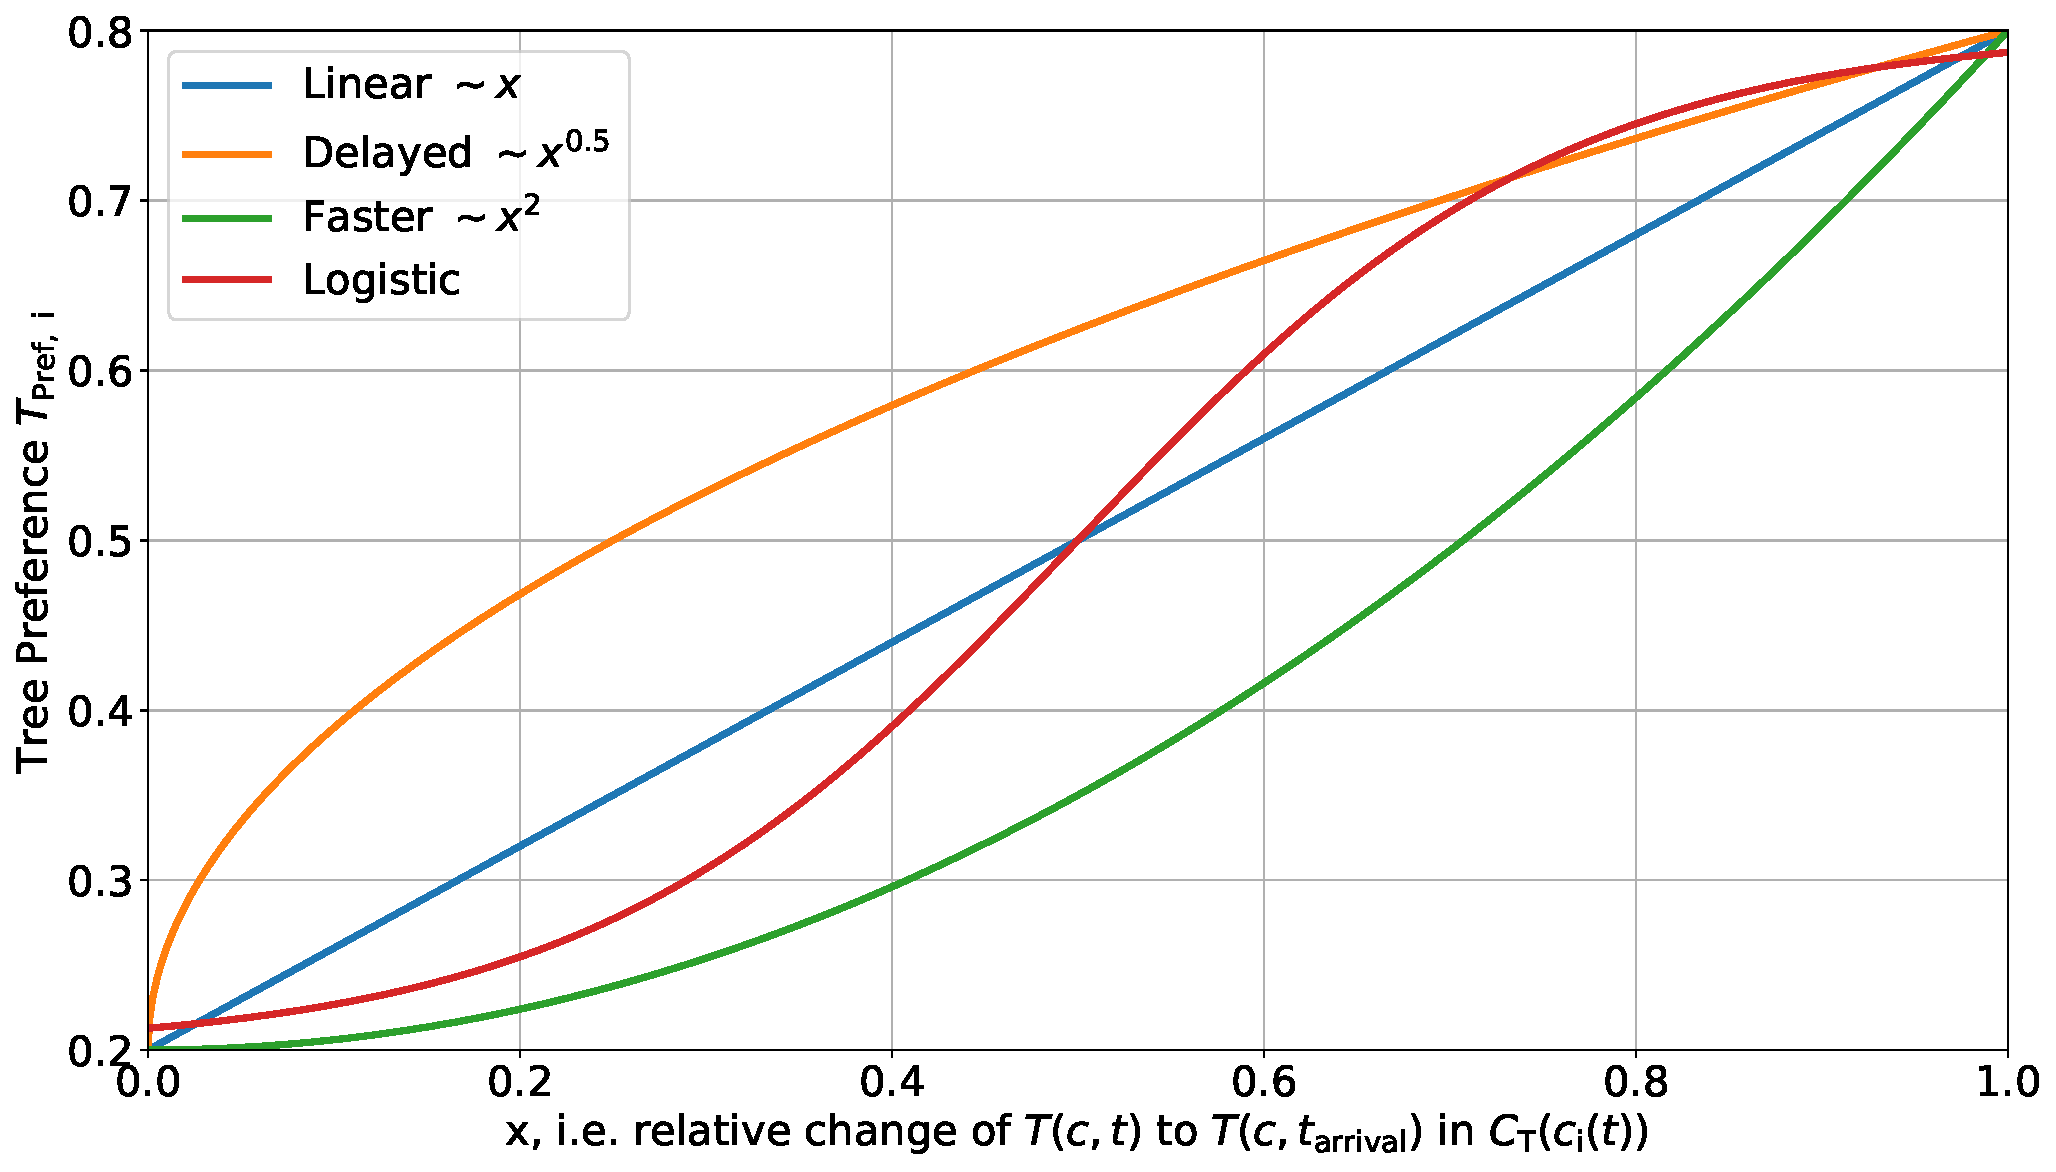
\includegraphics[width=\textwidth]{images/TPref}
	\caption{The relation of an agent's tree preference, $T_\text{Pref, i}(t)$, to relative changes in the local tree density for the four considered adaptive strategies $f_\text{Tree Pref}$ with $x$ given in equation~\ref{eq:TPref}.}
	\label{fig:TPref_T}
\end{figure}
The tree preference is cut off at certain minimum and maximum thresholds, assuming an agent can not live purely off trees (and associated derivate products), but, at the same time, some tree cutting is always required even for maximum agricultural production (e.g.\ as cooking wood or for tools). 
Here, I choose: 
\begin{equation}
T_\text{Pref, min} = 0.2 \quad \text{and} \quad T_\text{Pref, max} = 0.8
\end{equation} 
In the standard setting in this model, I use the linear relation and, hence, 
\begin{equation}
	T_\text{Pref, i}(t) =  \frac{\sum_{\tilde{c} \in C_{T}(c_{\rm i}(t)) } \, T(\tilde{c}, t)}{\sum_{\tilde{c} \in C_{T}(c_{\rm i}(t))} \, T(\tilde{c}, t_\text{arrival}) } \cdot (T_\text{Pref, max}-T_\text{Pref, min}) + T_\text{Pref, min}
\end{equation}
The initial agents start with maximal tree preference ($T_\text{Pref, i}(t=t_\text{arrival}) = 0.8 \ \  \forall \ i$), which then (in general) decreases slowly as the (local) deforestation progresses.

\paragraph{Resource Requirements}
An agent's required total resource uptake per year increases with the population size and the tree preference calculated after the harvest in the previous year.
Hence, the resource requirements of tree harvest, $T_\text{Req, i}(t)$, and farming produce, $F_\text{Req, i}(t)$, are 
\begin{equation}
T_\text{Req, i}(t) = T_\text{Pref, i}(t-1) \cdot pop_{\rm i}(t) \cdot T_\text{Req, pP} \, 
\end{equation}
and, similarly, 
\begin{equation}
F_\text{Req, i}(t) = (1-T_\text{Pref, i}(t-1)) \cdot pop_{\rm i}(t) \cdot F_\text{Req, pP}\, , 
\end{equation}
where $T_\text{Req, pP}$ is the constant tree requirement per year per person in absence of agriculture and $F_\text{Req, pP}$ is the constant required agriculture production per person in the absence of tree cutting.

%\paragraph{Tree Requirement per Person}
The tree requirement per person (in the absence of farming), $T_\text{Req, pP}$, in principle depends on a multitude of factors and was presumably heterogeneous between agents.
E.g.\ if agents used sugary sap from cut tree trunks as freshwater replacement (as suggested by \citet{Mieth2015}), they would require a much larger number of trees.
Here, I use a constant parameter of 
\begin{equation}
T_\text{Req, pP} = 5\, \frac{\text{Trees}}{\rm person\cdot yr}
\end{equation}
for all agents (for the standard model settings) based on the maximum harvest rate used in \citet{Brandt2015}, ca.\ $3$ to $7$ trees per year\footnote{\citet{Brandt2015} use a only half of the initial trees before arrival of the first settlers, though)}. 
However, I also explore a scenario with doubled tree requirement per person per year.
%In the standard run I am using $5$ Trees per Person per year. However, I vary this parameter in a sensitivity analysis (see Section \ref{sec:SensitivityAnalysis}).

%\paragraph{Farming Requirement per Person}
The requirement of farmed land per person (in the absence of tree cutting), $F_\text{Req, pP}$, crucially determines the overall carrying capacity of the human population.
\citet{Puleston2017} simulate the nutritional productivity of farming on well-suited land (as defined in Section \ref{sec:CreateMap}) for two different environmental scenarios of Nitrogen fixation in the soil, i.e.\ the rate at which Nitrogen is renewed, which represents a major uncertainty in their model\footnote{I do not consider fallowing as farming practice to increase productivity of arable land, as this, in general, reduces the productivity per total occupied area needed for each individual (see Table 1 in \citet{Puleston2017}).}.
This can be converted into the land required by one individual using the nutrition content of sweet potato\footnote{$1\, \rm{t/yr}$ roughly sustains $1$ individual in the absence of other food sources}: 
\begin{equation}
F_\text{Req, i}(t) = \begin{cases}
	0.5 \, {\rm \frac{acre}{person} } & \text{ for high N fixation} \\
	1.7 \, {\rm \frac{acre}{person} } & \text{ for low N fixation} \\
 \end{cases}
\end{equation}
However, the actual amount of required land per individual in the model is higher since all acre have less than $100\%$ relative yield (see definition of farming productivity indices $F_\text{PI}(c)$ and Figure \ref{fig:Map_agric}).

In summary, the resource requirements for trees (in absolute numbers) and farming produce (in acres of farmed sites with $100\%$ yield) are agent-specific, yearly varying features depending on the population size, reflecting the state of last year's local environment via the tree preference, and which can be tuned through the global parameters $T_\text{Req, pP}$ and $F_\text{Req, pP}$.

% Topic: Fishing Agents constrained by a tabu 
\paragraph{Fishing}
The model, furthermore, allows for open-ocean fishing as a replacement for farming for some agents living near the Anakena coast.
Instead of farming sites, these fishers gain sufficient agricultural resources by going out to sea on large canoes.
Excavations prove that shellfish, fish and even porpoise were a major part of the Easter Islanders' diet during the first settling phase \citep{Bahn2017}.
However, over time, these natural resources became increasingly scarce and many species even went extinct due to human predation, with open-ocean fish eventually vanishing from the diet of the Rapa Nui \citep{Diamond2011}.
As a resource management institution the Easter Island society installed taboos on the harvest of natural resources \citep{Good2006}. 
Fishing was mainly restricted to members of a specific chiefdom (`Miru') living at Anakena Beach \citep{Bahn2017} who would then presumably trade with others.
%According to \citet{Bahn2017} or \citet{Diamond2011}, sea fish vanished from the Easter Island typical diet by \TODO.
Hence, in the model, every agent up to a maximum of $N_\text{Fisher, Max} = 10$ (i.e.\ typically less than $400$ individuals) living within farming radius, $r_{\rm F}$, distance of Anakena Beach (in cell $c_{\rm Anakena}$) automatically becomes a fishing agent
\begin{equation}
 	c_{\rm i} \in C_{\rm F}(c_{\rm Anakena}) \  \cup \ N_\text{Fishers}<N_\text{Fisher, Max} \quad \Rightarrow \text{Agent }i\text{ becomes a fisher}
\end{equation}
%At time $t_\text{taboo fishing}=$\TODO a taboo is put in place externally.
%Consequently no new fishing agent's are accepted .
% letting only \TODO those agents already pursuing fishing to continue but allowing no further agents to enter this resource stock. 
While I assume that open-ocean fish supply is unlimited for those living at Anakena Beach, the major constraint for the fishers is the requirement for trees.
Since e.g.\ the construction of canoes or firewood presumably increased the tree requirement of these agents, I increase the minimum tree preference to
\begin{equation}
T_\text{Pref, min}|_\text{fisher} = 0.5
\end{equation} 
rather than $T_\text{Pref, min} = 0.2$ for farming agents.
Hence, while fishing agents near Anakena Beach do not have any farming requirements due to access to an unlimited resource stock from the sea, the correspondingly higher requirement for trees and an externally introduced restriction on their number both limit the exploitation of open-ocean fishing.

\FloatBarrier
\section{Agent-Environment Interaction} \label{sec:Harvest}
% TOpIC: HARVEST GENERAL
\paragraph{Sequence of Events}
In an update step in year $t$, an agent first determines the required amount of trees, $T_\text{Req, i}(t)$, and agricultural production, $F_\text{Req, i}(t)$, (as described in Section \ref{sec:agentprops}) and then acquires sufficient resources (if available) by interacting with the local environment, by first occupying farming sites and then removing trees.
This interaction is described in the remaining Section.
The sketch in Figure~\ref{fig:treeburning} shows an example of the process of deforestation and consequent replacement by farming in a cell.
\begin{figure}
	\centering
	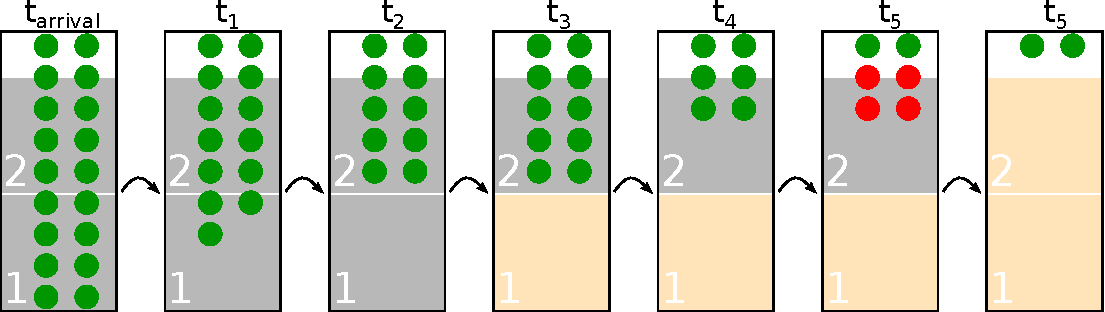
\includegraphics[width=\textwidth]{images/SketchABM2/burningSketch.pdf}
	\caption{Sketch of an exemplary deforestation procedure (by arbitrary agents) in a cell $c$ (black box) with an area of $2.3\, \rm{acres}$.
		The cell is arable, with $F_{\rm PI}(c)>0$ and, thus, provides $A_{\rm acres}=2$ acres for potential farming (grey squares).
		Initially at $t_{\rm arrival}$, the cell has $18$ trees (carrying capacity).
		At some time $t_{\rm 1}$, after deforestation $13$ of these trees still exist. 
		An Agent $a$ removes $3$ trees from the cell (\ra $t_{\rm 2}$). 
		Subsequently, Agent $b$ then occupies the now cleared site ($1\, {\rm acre}$) on cell $c$ for farming (\ra $t_{\rm 3}$). 
		Agent $c$ cuts another $4$ trees (\ra $t_{\rm 4}$).
		And finally, at $t_{\rm 5}$, an agent $d$, needs to occupy more sites to fill its farming requirement and cannot find any other arable, unoccupied site in $C_{\rm F}(c_c)$ except for the second site in cell $c$. 
		However the agent needs to burn $4$ more trees (red) before being able to occupy the second acre on this cell (\ra $t_{\rm 5}$).}
	\label{fig:treeburning}
\end{figure}

\paragraph{Farming}
An agent occupies arable land unit sites, $A_\text{F, i}(t)$, with a fixed area of $1\, \text{acre}$ associated to one cell and obtains a yearly farming produce of
\begin{equation}\label{AProd}
F_\text{i}(t) = \sum_{a \, \in \, A_\text{F, i}(t)} \, F_{PI}(c(a))\ ,
\end{equation}
where $a$ denotes a farmed acre and $c(a)$ is the corresponding cell of this acre\footnote{Note, for fishers $F_\text{i}(t) = F_\text{Req, i}(t)$ holds immediately without farming and occupying sites.}.
Agents keep all their currently occupied sites $A_\text{F, i}(t)$ until the next year. %, i.e.\ $acres_{\rm i}(t+1) = acres_{\rm i}(t) + new\_acres(t+1)$.
If, over time, an agent $i$'s farming requirement, $F_\text{Req, i}(t)$, increases e.g.\ due to population growth, decrease of the tree preference or erosion and degradation of the soil of one of its occupied sites, and consequently the farming produce of the previous year would be insufficient, then the agent needs to occupy more arable sites: 
\begin{equation}
F_\text{i}(t-1) < F_\text{Req, i}(t) \ \Rightarrow \ \text{Extend } A_\text{F, i}(t) \text{ and, thus, } F_\text{i}(t) {\rm !}
\end{equation}
%Then the agent occupies more sites extending $A_\text{F, i}(t)$ and, thus, increasing the produce $F_\text{i}(t)$ accordingly.
In the search for new farming sites, an agent first considers only sites in well-suited cells, i.e.\ $c \in C_\text{F}(c_\text{i}(t))$ with $F_\text{PI}(c)=F_\text{PI}|_\text{well}$, in order to maximise farming efficiency.
An acre in an arable cell can only be occupied (or added to $A_\text{F, i}(t)$) if at least this area of $1\, {\rm acre}$ is cleared off trees and not already occupied. 
Assuming that the trees are evenly distributed on the cell's area, the condition can be calculated as 
\begin{eqnarray}
%& \text{Treeless Area\,[acre]} - \text{Occupied Acres\,[acre]}  & \geq 1  \\
%\Leftrightarrow & 
\left( 1 - \frac{T(c,t)}{T(c,t_{\rm arrival})} \right) \cdot A(c) - \mathbf{A}_\text{F}(c, t) & \geq   1
\label{eq:BurningCond}
\end{eqnarray}
where the first term is the treeless area in ${\rm acres}$ and the second term, $\mathbf{A}_\text{F}(c, t)$, is the number of already farmed acres (by any agent) in cell $c$.%(equation~\ref{eq:occupied}).

If there are no well-suited sites left that fulfil this condition, the agent uses the slash and burn method to reduce the number of trees $T(c,t)$ of a well-suited cell $c$ (with at least one unoccupied acre).
The agent starts burning trees on the cell that requires the least amount of trees removed (without leading to erosion of the cell) for the condition to hold.
Burning trees and occupying sites continues until the farming requirement of the agent is satisfied or no more well-suited acres are available (even if this leads to erosion of the cell).
The use of fires to clear space is supported by the extensive charcoal record starting with the period of intensified agriculture \citep{Mieth2015}. 
Here, I assume that if space is required for farming at time $t$, trees are burned directly and not used to fill the tree requirement (assuming this is a more gradual process over the year than the instantaneous burning).
%felled and used (e.g.\ for extraction of the sugar sap) before burning and consequent agricultural use of the land \citep{Mieth2015} or slash and burn method was used directly to clear space as necessary next to tree harvest %(e.g.\ indicated by \citet{Bahn2017}). % Bahn: ``fires directly accompanied by agriculture''
If, all well-suited sites within $C_{\rm F}(c_{\rm i}(t))$ are occupied, but the agent's farming produce does not yet meet the requirement ($F_\text{i}(t)<F_\text{Req, i}(t)$), the agent also occupies sites on eroded cells and then on poorly suited cells in the same procedure.

\paragraph{Tree Harvest}
After filling the farming requirement, the agent then cuts trees according to its tree requirement $T_\text{Req, i}(t)$.
An agent $i$ selects random cells $c\in C_{\rm T}(c_{\rm i}(t))$ with uniform probability and successively removes trees from these cells until the number of cut trees, $T_\text{i}(t)$ matches the requirement $T_\text{Req, i}(t)$ or no further trees are present in $ C_{\rm T}(c_{\rm i}(t))$. 
Unlike farming, where occupied sites are kept and re-used (with the same productivity index) in the next year, the agent obviously needs to find new trees every year.
%Therefore, if tree regrowth is disabled, this tree harvest represents a non-renewable resource dependency of the Easter Island society.
While the agent's adapt their harvest behaviour via the tree preference as this non-renewable resource is depleted over time, a minimum amount of trees is always required and, hence, there's no equilibrium existence of human population without tree regrowth.

\paragraph{Happiness Index}
The agents internal state is summarised in a happiness variable, $h_{\rm i}(t)$, that reflects the success of the harvest of trees and farming produce each year.
Here, an agent $i$'s happiness $h_\text{i}(t)$ depends on the ratios of the cut trees, $T_\text{i}(t)$, and farming produce, $F_\text{i}(t)$, w.r.t.\ the requirements determined beforehand, $T_\text{Req, i}(t)$ and $F_\text{Req, i}(t)$, respectively, in each year.
%Assuming that both requirements determine  the tree requirement and the agriculture requirement is equally important to the agent, the happiness is simply the minimum of the fraction of requirements that could be filled:
By assuming that both resources are equally indispensable for the agent, the happiness is equal to the smaller of the two fractions:
\begin{equation} 
h_\text{i}(t) = {\rm min} \left( \frac{T_\text{i}(t)}{T_\text{Req, i}(t)}, \, \frac{F_\text{i}(t)}{F_\text{Req, i}(t)} \right)
\label{eq:h_i}
\end{equation}
If both requirements are filled for agent $i$, the happiness is maximal,  $h_\text{i}(t)=1$.
However, if either $T_\text{i}(t)=0$ or $F_\text{i}(t)=0$, $h_\text{i}(t)=0$ follows regardless of the success in harvesting the other resource.
I assume that households have some resilience to a decline in harvest success (e.g.\ by storing food in more successful years), and, hence, define a memory happiness $H_\text{i}(t)$ as
\begin{equation}
H_\text{i}(t) = \begin{cases} 
				h_\text{i}(t) & \text{ if } h_\text{i}(t)\geq h_\text{i}(t-1) \\
				\frac{h_\text{i}(t) + h_\text{i}(t-1)}{2} & \text{ if } h_\text{i}(t)<h_\text{i}(t-1) 
		\end{cases}
\end{equation}
If an agent's harvest success decreases (due to resource scarcity), its memory happiness $H_{\rm i}(t)$ decreases monotonically.
If e.g.\ all trees were to suddenly vanish within a year, an agent would have two years before its memory happiness reaches its minimum $H_\text{i}(t) = 0$.
However, if harvest success increases (e.g.\ due to moving the settlement to a better location), the memory happiness takes on the new happiness value immediately.
As an indicator for successful resource acquisition, the memory happiness $H_\text{i}(t)$ determines the possible responses of agent $i$ to the harvest, which I describe in the following Sections \ref{sec:PopGrowth} and \ref{sec:Moving}.

%\section{Responses of Agent Features Following the Resource Acquisition}\label{sec:Reaction} 
\FloatBarrier
\section{Population Growth Module}\label{sec:PopGrowth}
\paragraph{Stochastic, Discrete Population Growth}
Following the interaction between the agent and the environment through farming and tree cutting, the agent's population size $pop_{\rm i}(t)$ adapts. 
The net (positive or negative) growth rate of the agent's population at a specific time depends only on the memory happiness and, thus, harvest success:
\begin{equation}\label{eq:popgrowthcontinuos}
pop_{\rm i}(t+1) = (1+g(H_{\rm i}(t))) \cdot pop_{\rm i}(t)
\end{equation}
In fact, instead of assuming continuous growth or decline according to this growth rate, $g(H_{\rm i}(t))$, the population dynamics is implemented as a discrete, stochastic process.
Each individual of the household agent has a $|g(H_{\rm i}(t))|$ probability to die if $g(H_{\rm i}(t))<0$, or %a $g(H_{\rm i}(t))-1$ chance 
to reproduce (i.e.\ adding one individual to the household/agent) if $g(H_{\rm i}(t))>0$.
The population size stays constant at $H_{\rm i}(t) = H_{\rm equ}$ with $g(H_{\rm equ}(t))=0$. 
This results in a stepwise growth/decline of the population in which each agent's population size trajectory is a single realisation of the stochastic process which on average matches the continuous dynamics in equation~\ref{eq:popgrowthcontinuos} (compare e.g.\ with \cite{Bungartz2009}).
Note, $g(H_{\rm i}(t))$ represents a harvest dependent stochastic, discrete \textit{excess} growth or decline rate. 
I assume that `base' (i.e.\ for $H_{\rm i}(t) = H_{\rm equ}$ and, thus, $g(H_{\rm equ})=0$) deaths and births average out for each year in spite of the fact that this too is a stochastic discrete process \citep{Bungartz2009} and hence, should introduce even more variation.
Figure \ref{fig:realisationsofpopgrowth} in Appendix \ref{sec:PopGrowth} shows a few different realisations of a discrete, constant (excess) growth scenario with rate $g(H_{\rm i}(t)=1)=0.7\%$ (i.e.\ with unlimited resource availability) in comparison with the continuous growth.

\paragraph{Growth with Unlimited Resources}
There is an excessive debate about the initial growth rate of the Easter Island population after the arrival of a small number of Polynesians.
This corresponds to the growth rate, $g(H_{\rm i}(t))$, without resource constraints and, thus, $H_{\rm i}(t)=1$.
Parameters used in the literature range from $0.7\%$ per year \citep{Bahn2017} or `always below $1\%$' \citep{Brander1998} to exceeding $3\%$ \citep{Hunt2007} for short periods of time or $2.3-4.5\%$ \citep{Brandt2015}.
Depending on the proposed chronology, researchers have to make very contrary assumptions on the population growth in order to fit the population dynamics to the few undisputed facts about the pre-historic civilisation on Easter Island. 
If an arrival around $1200\, \text{A.D.}$ is assumed (as in \citet{Hunt2007} or \citet{Brandt2015}), a large population growth is unavoidable\footnote{E.g.\ as it seems impossible that only a few hundred inhabitants in the 13th to 16th century could have created several hundred Moai statues (and caused a massive alteration of the island's environment)}.
On the other hand, slower initial population growth needs to be assumed in studies proposing earlier arrival dates (around $800\, \text{A.D.}$(e.g.\ \citet{Bahn2017}) or even as early as $400\, \text{A.D.}$ (\citet{Good2006} and \citet{Brander1998})), given that archaeological data indicates an intensification of human activity, which suggests a large population size, only starting after $1200\, \text{A.D.}$ (e.g.\ \citet{Bahn2017}) and \citet{Hunt2007}).
Other theories, such as multiple, distinct periods of population growth and declines have been put forward (e.g.\ \citet{Cole2008}), but do not seem to be common in the context of Easter Island.
%Archaeological data, e.g.\ charcoal evidence, however, suggests a period of intensification of human activity starting after $1200\, \text{A.D.}$ (e.g.\ \citet{Bahn2017}) and \citet{Hunt2007}).
%Hence, these studies assume a slow but continued population growth starting with the `early' arrival.% way before $1000\, {\rm A.D.}$.% up to a peak population in $1300-1700\, \text{A.D.}$.
%, one has more freedom in choosing the initial growth rate.
%especially considering that there might have been several phases of population declines as proposed in \citet{\TODO Bahn2017}. 
%One could imagine that after initial fast growth of the population after an early arrival, through fertility control a steady population size was reached below Easter Island's resource carrying capacity. 
%Archaeological and charcoal data, however, suggest an intensification of human activity (and its impacts on the environment) only at around 1200 \citet{Hunt2007} and very little environmental impact before that.
%Most researchers rather assume a slow but continued population growth from an early arrival to a peak population around 1300-1700 (e.g.\ \citet{Brander1998}, \citet{Bahn2017})
Following \citet{Bahn2017}, I choose an early arrival date here ($t_\text{arrival}=800\, A.D.$), as described before, and, thus, a slow growth rate (in one year) in the case of unlimited resource access and, therefore, continuously happy agents: 
\begin{equation}
	g(H_\text{i}(t)=1) = 0.7\% \ .
\end{equation}

\paragraph{Growth or Decrease with Limited Resources}
The dependency of the population growth or decline rate, $g(H_{\rm i}(t))$, in the case of limited resources, $H_{\rm i}(t)<1$, is a further uncertainty in modelling human-resource interactions in general.
\citet{Lee2008} and \citet{Puleston2008} constructed a food-limited demography model applied to simulating the Easter Island society and farming constraints in \citet{Puleston2017}. 
Here I use a strongly simplified assumption of this model to parametrise the impact of non-optimal harvests on the population dynamics. 
The authors derived age-dependent survival and fertility rates, which are both S-shaped curves w.r.t.\ the food availability (i.e.\ high in the case of unlimited food availability and low in the case of scarce food availability).
Since, I do not consider (age-stratified) structures below the agent/household level, I simply assume a net growth rate with the same shape as the survival and fertility rates in \citet{Lee2008}.
\begin{equation}
g(H_\text{i}(t)) \sim \text{CDF}(\Gamma_\text{Dist}(shape, scale=0.1))
\end{equation}
where $\text{CDF}(\Gamma_\text{Dist})$ is the cumulative density function of the Gamma distribution (characterised by shape and scale parameter) with scale fixed as in \citet{Lee2008}.
I then tune the shape parameter of this function to obtain the same   equilibrium point $g(H_\text{i}(t) =H_\text{equ})=0$ as \citet{Puleston2017}, at which the population size remains constant:
\begin{equation}
H_\text{equ}=0.6883 \quad \text{with } g(H_\text{i}(t) = H_\text{equ})=0   \ .
\end{equation} 
In order to test sensitivity of this parametrisation, I also investigate a larger shape parameter $shape^*=3$, which leads to a less resilient population size when resource scarcity sets in.
In this alternative, less resilient scenario, the growth rate declines faster if $H_\text{i}(t)$ decreases and the equilibrium point is transgressed already at a higher happiness value $H_\text{equ}^*=0.84$.  %$g(H_\text{i}(t)=H_\text{equ}^*)=1$
The amplitude of the resulting function (for both scenarios) is scaled to give the chosen reproduction rate under unconstrained food supply from last paragraph 
$g(H_\text{i}(t)=1)=0.7\%$.
Figure \ref{fig:growthrate} shows the resulting two parametrisations of an agent's population growth rates (standard setting in blue and less resilient setting in red) with the happiness regime for net growth, $H_\text{i}(t) > H_{\text equ}$ (with a maximum of $g(H_\text{i}(t)=1)=0.7\%$) and the regime for net decline of the population size, $H_\text{i}(t) > H_{\text equ}$.
%(for $H_\text{i}(t)>H_\text{equ}$, with a maximum of $g(H_\text{i}(t)=1)=1.007$) and decline (for $H_\text{i}(t)<H_\text{equ}$) .
\begin{figure}
	\centering
	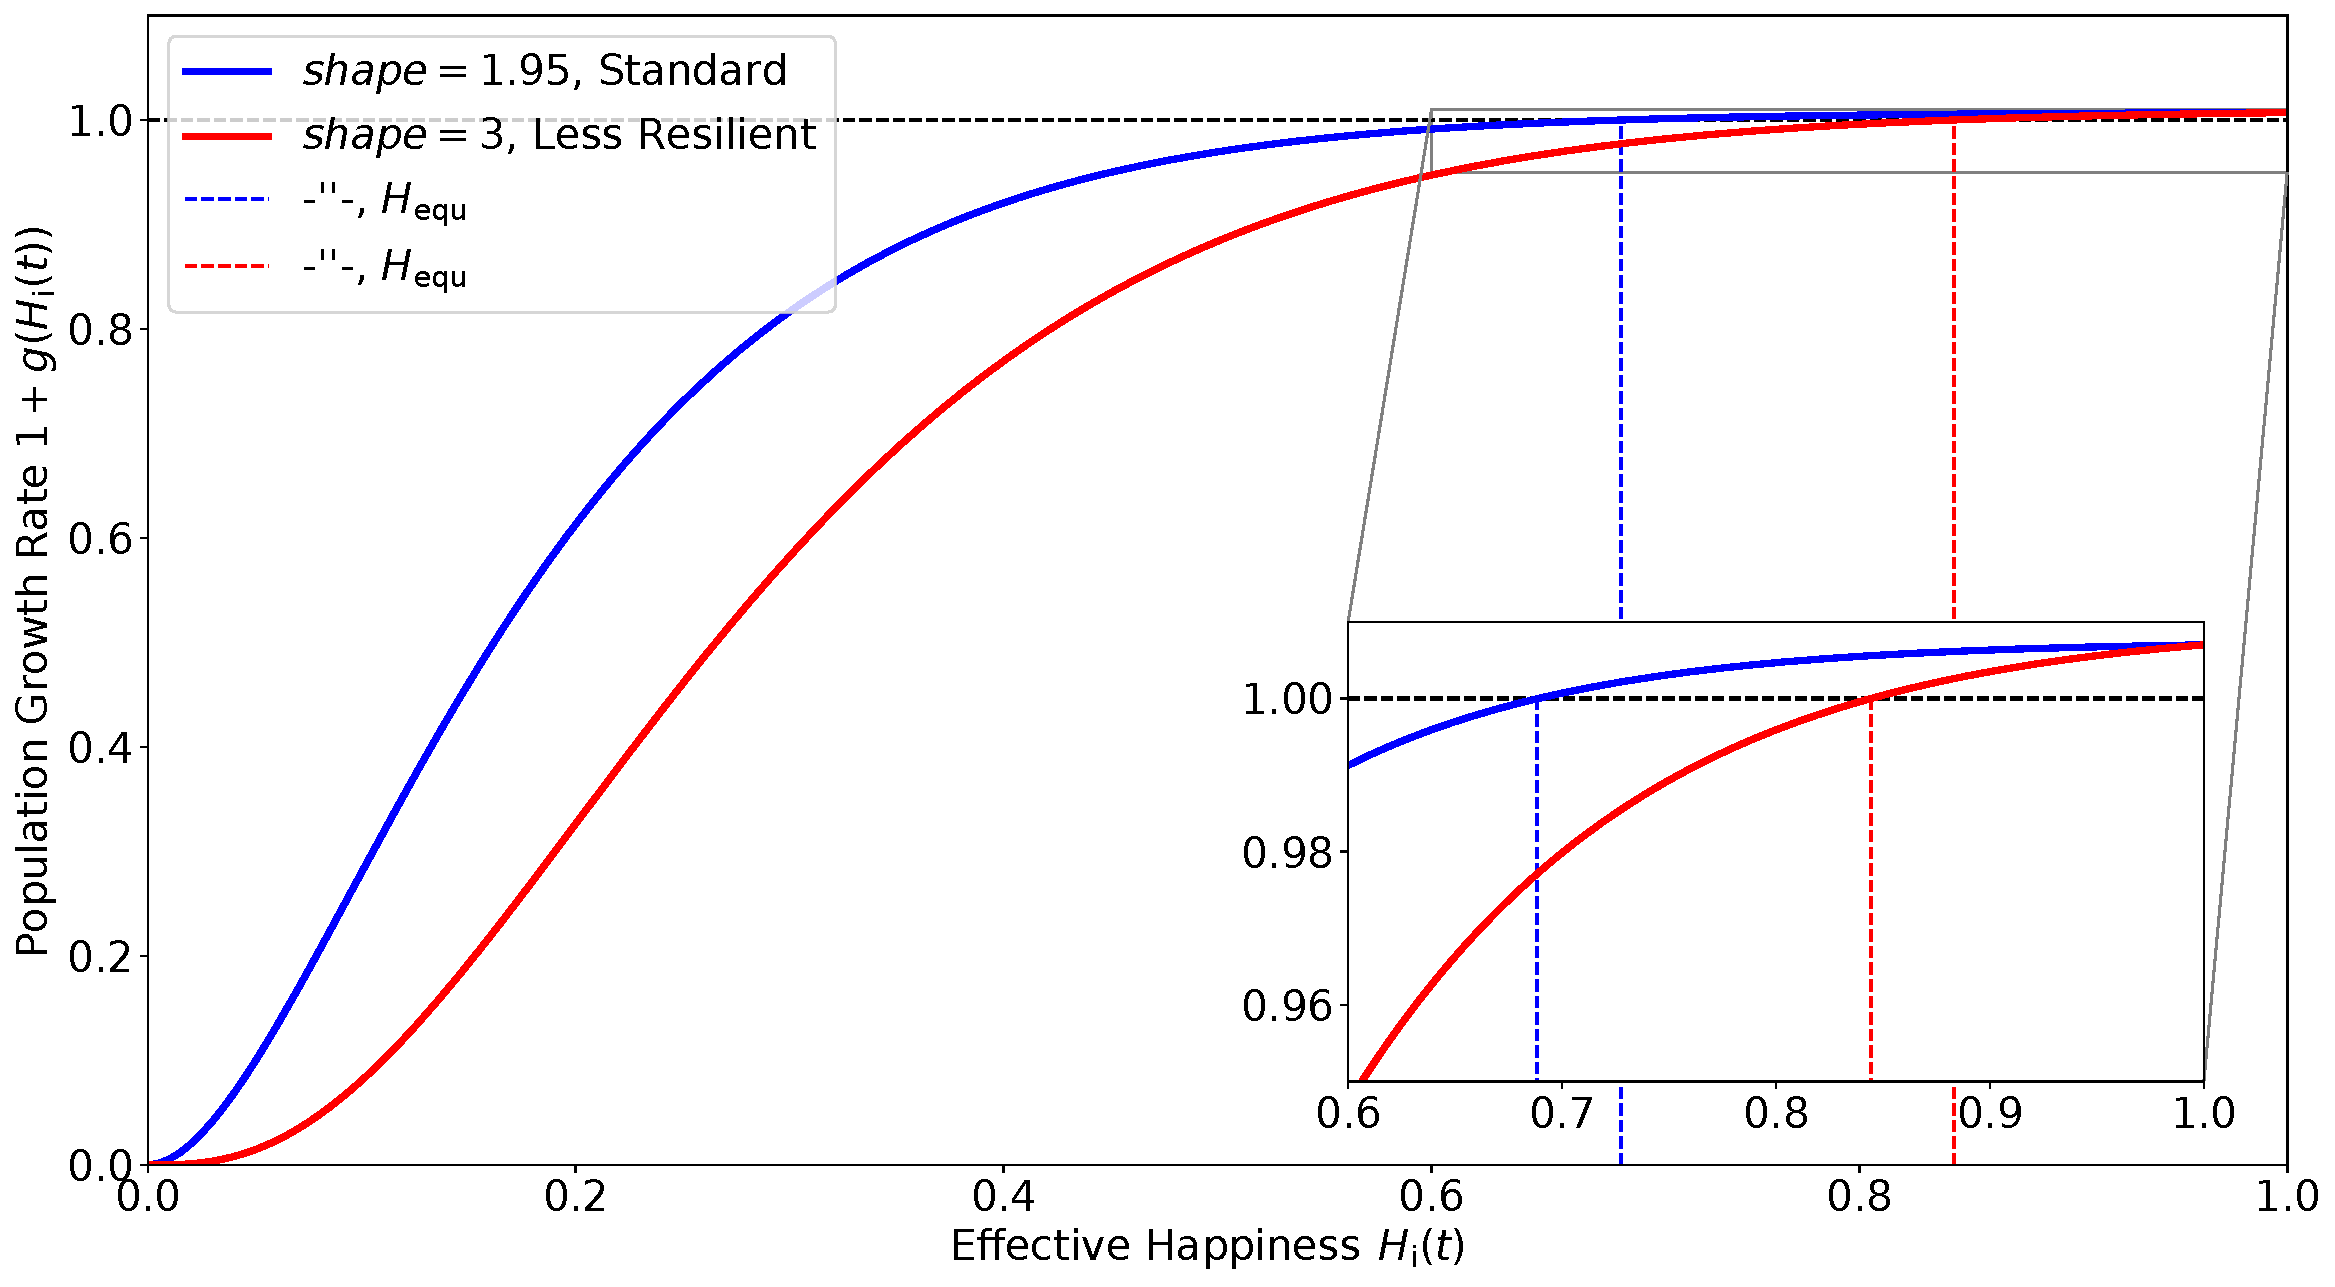
\includegraphics[width=\textwidth]{images/populationchange_g}
	\caption{The growth rate of an agent's population size as a function of its memory happiness $H_{\rm i}(t)$. Functional dependence follows simplified assumptions made in the food-limited demography model in \citet{Lee2008}, \citet{Puleston2008}, and \citet{Puleston2017}. In the standard scenario (red) the agent's population size grows if $H_{\rm i}(t)>H_{\rm equ}=0.6883$ and declines for smaller $H_{\rm i}(t)$. An alternative, less resilient scenario is also tested, with a smaller population growth regime of $H_{\rm i}(t)>0.84$. The maximum growth rate in the case of maximum happiness (and thus unconstrained resource availability) is $g(H_{\rm i}(t)=1)=0.7\%$.}
	\label{fig:growthrate}
\end{figure}
%There are two regimes of population dynamics: a population growth for $H_\text{i}(t)>H_\text{equ}$ with maximum $g(H=1)=1.007$, and a decline for 
%At $H=1$, the households population grows with rate $1.007$, as tree or agricultural land availability decreases, the agent's smoothed happiness decreases and so does the growth rate. If $H<0.6883$, the population size decreases.

% Topic SPLITTING THE AGENT
\paragraph{Splitting or Removal of an Agent}
There are upper and lower limits to the population size of an agent, causing it to split or disperse.
If the population size $pop_{\rm i}$ of an agent $i$ falls below a certain threshold $pop\_{\rm min} = 6$, the agent $i$ is removed and the remaining individuals are adopted by other households chosen randomly within the moving radius distance, $r_{\rm M}$ ($C_{\rm M}(c_{\rm i})$ defined later).
If the household's population becomes too large, a subgroup splits from it forming a new agent.
According to \citet{Bahn2017}, settlements found in archaeological excavations consisted of two to three dwellings, the basic domestic units (e.g.\ caves or stone houses). 
Assuming that roughly a dozen people can live in such a dwelling, which would include the larger family, a household includes around $30$ ($2.5\cdot 12$) individuals.
In this model, if the population size reaches values requiring more than three dwellings, a dozen individuals splits off and starts a new settlement on a different location on the island. 
The stochastic splitting probability given an agent's population size is
\begin{equation}
Pr_{\rm splitting} = \mathcal{N}( \mu = pop_\text{max, mean}, \sigma = pop_\text{max, std})\ .
\end{equation}
with $pop_\text{max, mean} = 3.5 \cdot 12 = 42$ and $pop_\text{max, std} = 3$.
The remaining household abandons not required occupied farming sites.
The splitting agent, immediately moves to a new location determined by the moving process described in Section~\ref{sec:Moving}.
Hence, an agent represents a household of typically $12$ (with a lower limit of $6$) to $42$ individuals. % that acts independent of other agents.

\FloatBarrier
\section{Moving Module}\label{sec:Moving}
% When to move
\paragraph{Procedure and Condition for Moving}
Agents relocate their settlement as a reaction to either insufficient harvest success or after splitting from a large household to start a new settlement.
If, after the harvest, the agent's smoothed happiness is below the equilibrium point $H_\text{equ}=0.6883$ (in the standard setting), i.e.\ net negative growth $g(H_\text{i}(t))\leq 0$, the agent searches for a new location.
The agent first chooses a cell within a certain radius according to probabilities that indicate how high the agent evaluates this location in several different categories.
Within this new cell, the agent chooses a location with uniform probability and settles there.

% How to calculate moving radius
\paragraph{Moving Radius}
In the initial phase of the simulation, agents can choose new locations from all cells on the island\footnote{Except for the initial settlers who are assumed to settle close to the landing spot, Anakena Beach}.
However, if a certain total population size is exceeded (here $\mathbf{pop}(t)\geq \mathbf{pop}_\text{restricted moving} = 5000 \, \rm{people}$), I externally enforce a restriction of the agents' ability to move around freely and, therefore, new settlements are only allowed within a certain radius of the agent's old location.
When relocating the settlement, an agent $i$, thus, chooses from cells:
%Thus, the cells considered as potential new location for an agent $i$ are
\begin{equation}
C_{M}(c_{\rm i}, \mathbf{pop}(t)) = 
\begin{cases}
\{\tilde{c} \ | \ \tilde{c}\text{ on island}\} & \text{ if } \mathbf{pop}(t) <5000 \\
\{\tilde{c} \ | \ | | \vec{\tilde{c}} - \vec{x_{\rm i}}(t) | |
%\begin{pmatrix} \tilde{c}_x \\ \tilde{c}_y \end{pmatrix}  - \begin{pmatrix}x_i\\ y_i \end{pmatrix} 
\leq r_{\rm M} \} & \text{else} 
\end{cases}
\end{equation}
with radius $r_{\rm M} = 5\, {\rm km}$.

% Topic: It's a decision making process.
%Determining the new location for an agent represents a decision-making process through evaluation of sites by the agent.
\paragraph{Deciding on the New Location}
In a semi-rationale decision making process the agents decide on a new location by evaluating cells $c$ within $C_{\rm M} (c_{\rm i}, \mathbf{pop}(t))$ according to probabilities inferred from several different penalties:
%The calculation of the probability to move to a specific cell bases on penalties from the following categories: 
$P_{\rm G(c)}$ for geographical constraints, $P_{\rm W}(c)$ for distance from freshwater, $P_{\rm D}(c)$ for population density, $P_{\rm T}(c)$ for tree availability, and $P_{\rm F}(c)$ for farming land availability.
High penalties represent unfavourable conditions (in the specific category) for settling in the specific cell.


%TOPIC: LOGISITIC FUNCTIONS
\paragraph{General Calculation of Penalties}
Penalties for each category $P_{\rm X}$ ($X=\{\text{G,\, W, \, D,\, T,\, F}\}$) are calculated via logistic functions depending on one characteristic evaluation variable $x$ ranging from $x_{\rm min}$ to $x_{\rm max}$.
In reality such an evaluation would typically depend on more than one variable and might have complex functional behaviour.
However, the assumption made here is a plausible simplification given that with the logistic function there is a range of values of the evaluation variable indicating favourable conditions (with similarly negligible penalties) and a range of values indicating unfavourable conditions (with similarly high penalties)\footnote{For example an agent might assign the same penalty to two locations $100\, \text{m}$ and $500\, \text{m}$ away from a large freshwater source. If instead the nearest lake is too far away from the agent to rely on it for everyday use, alternative sources have to be found, regardless of whether the distance is $5$ or $10\, {\rm km}$ and therefore, the penalty is similarly high.}.
I determine the shape of the function of $P_X$ of variable $x$ through `thresholds' $x_{\rm P0.01}$ and $x_{\rm P0.99}$ indicating the value of $x$ at which the penalty $P_{\rm X}$ is smaller than $1\%$ (favourable conditions) or larger than $99\%$ (unfavourable conditions), respectively, in this category $X$.
The penalty $P_{\rm X}$ in a cell $c$ with value $x(c)$ is then
\begin{eqnarray}\label{eq:P_X(c)}
	P_{\rm X}(c) & = & \frac{1}{1+\exp\left( - k_{\rm X} (x(c)-\frac{x_{\rm P0.01}+x_{\rm P0.99}}{2}) \right)} %= \\
%		& = & \begin{cases}
%	<0.01  & \text{ for }x_{\rm min}<x(c)<x_{P0.01} \\
%	\text{?}  & \text{ for } x_{P0.01}\leq x(c) \leq x_{P0.99} \\
%	>0.99  & \text{ for }x_{P0.99}<x(c) < x_{\rm max} \\	
%	\end{cases}
\end{eqnarray}
where steepness $k_{\rm X}$ is 
\begin{equation}\label{eq:k}
k_{\rm X} = \left(\frac{x_{\rm P0.99}-{x_{\rm P0.01}}}{2}\right)^{-1} \cdot \log\left(\frac{0.99}{0.01}\right) \ .
\end{equation}
to fix the penalty to the respective values at thresholds $x_{\rm P0.01}$ and $x_{\rm P0.99}$.
This function is shown for a general case in Figure \ref{fig:logF}.
\begin{figure}
	\centering
	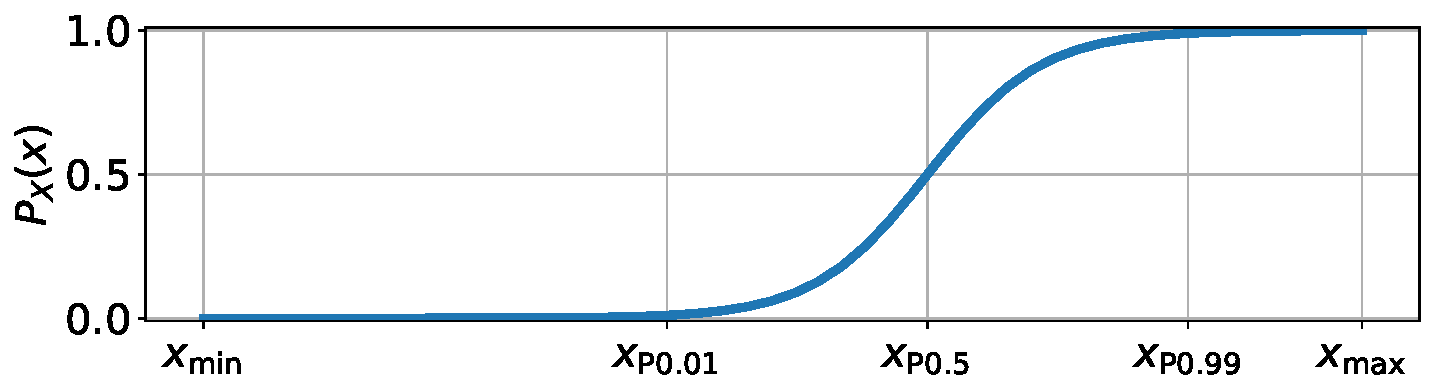
\includegraphics[width=\textwidth]{images/general_logF.pdf}
	\caption{General shape of the logistic function $P_{\rm X}(c)$ for a penalty for moving to a certain cell $c$ in the category $X$ ($\in\{\text{W, G, D, T, F}\}$). The penalty depends on a characteristic variable $x$, in combination with the thresholds, $x_{\rm P0.01}$ and $x_{\rm P0.99}$ (and $x_{\rm min}$ and $x_{\rm max}$) and, thus, the steepness parameter $k_{\rm x}$.}
	\label{fig:logF}
\end{figure}
For each category $X$, this logistic function has the same (relative) shape between $x_{\rm P0.01}$ and $x_{\rm P0.99}$. % given by $k_{\rm x}$. 
Hence, the sensitivity of penalty $P_X$ to differences in variable $x$ is determined by choosing $x_{\rm P0.01}$ and $x_{\rm P0.99}$, and thus, $k_{\rm x}$.
If the values of $x_{\rm P0.01}$ and $x_{\rm P0.99}$ are close, the function converges to a sigmoid function. 
If they are far apart, the function resembles a more linear increase of penalty $P_X$ with $x$.
For $x=\frac{x_{\rm P0.01} + x_{\rm P0.99}}{2}$ the penalty is $P_X = 50\%$.
Note, that if $x$ is chosen such that large values are favourable (e.g.\ for the tree and farming penalty), choosing values $x_{\rm P0.01}>x_{\rm P0.99}$ simply mirrors the logistic function in equation \ref{eq:P_X(c)} at its midpoint $x=\frac{x_{\rm P0.01}+x_{\rm P0.99}}{2}$ and all $<$ or $>$ signs accordingly.
This logistic dependence of penalties on a characteristic variable introduces non-linear evaluation of locations.

%The steepness $k_0$ can be chosen, such that the different cases of function $P_X(x)$ are reasonably close at the threshold values $x_{\rm P0.01/P0.99}$. 
%Here, I choose $k_0 = \left( \frac{x_{\rm P0.01}-{x_{\rm P0.99}}}{2}\right)^{-1}\cdot \log\left(\frac{0.01}{0.99}\right)$, giving $P_{\rm X(x=x_{\rm P0.01})=0.01$ and $P_{\rm X(x=x_{\rm P0.99}) = 0.99$.
%Higher $k_0$ results in a steeper increase of the penalty with $x$.
%Nevertheless, this choice for parametrising a complex decision making process as well as the values for the thresholds are very flexible. 
%Of course, we can not know how Easter Island households evaluated potential new settlement areas.
%Nevertheless, archaeological data as well as logic surely show that the island has been settled progressively, e.g.\ \citet{Bahn2017}. Hence, it can be very useful to understand what 
%However, it reflects a decision. 

% Following up: Penalty Categories and summary in sketch and table
%The parametrisation of evaluating new locations is, of course, strongly simplified. 
%First, the decision making typically depends on more than one evaluation variable per penalty category, as assumed here.
%Secondly, the functional dependency of penalty w.r.t.\ the evaluation variable in general is more complex than the simple logistic evaluation in equation~\ref{eq:P_X(c)}.
%However, assuming that advantages and disadvantages of a potential location (summarised in a single variable) play a non-linear role in the agent's decision making, the use of a logistic function seems reasonable\footnote{For example an agent might assign the same penalty to two locations $100\, \text{m}$ and $500\, \text{m}$ away from a large freshwater source. 
%If instead the nearest lake is too far away from the agent to rely on it for everyday use, alternative sources have to be found, regardless of whether the distance is $5$ or $10\, {\rm km}$ and therefore, the penalty is similarly high.}.

\paragraph{Parameter Choices} %for $\mathbf{P_{\rm X}(x)}$}
I determine the choice of the evaluation variable $x$ and thresholds $x_{\rm P0.01}$ and $x_{\rm P0.99}$ via plausible, heuristic arguments or estimates.
The following paragraphs point out the motivation for the specific variables for the agent's evaluation process and the threshold choices in the standard settings of the model for each penalty category $P_{\rm X}$ ($X=\{P_{\rm X}$ ($X=\{\text{G,\, W, \, D,\, T,\, F}\}$).
Table \ref{tab:x01x09} summarises the variables and corresponding thresholds that together with equation~\ref{eq:P_X(c)} determine the penalties $P_{\rm X}$ w.r.t.\ $x$ for all categories and thus the decision making of an agent when relocating the settlement.
%All of these contributions in a cell $c$ are then linearly combined to a total penalty for this cell $P_{tot}(c)$. 

%\begin{figure}
%	Logistic Functions
%	\label{fig:Logistic}
%\end{figure}

% TOPIC: Water Distance PEnalty
\paragraph{Distance from Freshwater}
There are very limited permanent sources of freshwater on the island, making it an important factor of settlement behaviour. 
Nearly all studies point out that the lakes inside the three volcano craters (Rano Kau in the South, Rano Rarakua in the East, and Rano Aroi in the North) are a dominant freshwater supply
\footnote{Other potential sources include pools in lava tubes and springs in the North Coast (all mentioned in \citet{Bahn2017}), an intermittent stream from Mount Terevaka, wells and water bubbles at low tide, and sugar cane juice (all mentioned in \citep{Diamond2011}), 
Additionally, \citet{Mieth2015} emphasizes the possibility to obtain a sugary sap from cut palm tree trunks, which could have replaced the need for freshwater for a large share of the population.
However, crater lakes are the most reliable (and accessible) large freshwater supply.}
and, thus, are `obvious centres for human activity' \citep{Bahn2017}.
%Topic Variable xC
Consequently, I assume that potential locations close to (large) lakes are more likely settled.
The evaluation variable $w$ is radially increasing with the distance to the nearest lake weighted by the area of it:
\begin{equation}
	w = min_{\text{lake}\in \text{[Kau, Raraku, Aroi]}} \left( \frac{||
		%\begin{pmatrix} c_x \\ c_y \end{pmatrix}  - \begin{pmatrix} \vec{lake}\\ y_i \end{pmatrix}
		 \vec{c}- \vec{lake}(t)||^2}{r_\text{lake}^2\pi} \right)
\end{equation}
%\begin{equation}
%	P_W(c) = \frac{1}{N} \cdot min_{\text{lake}\in \text{[Kau, Raraku, Aroi]}} \left( \frac{\text{dist(lake, c)}^2}{r_\text{lake}^2\pi} \right)
%\end{equation}
with $r_\text{Kau} = 506\, \rm{m}$, $r_\text{Raraku} = 170\, \rm{m}$, $r_\text{Aroi} = 75\, \rm{m}$ and $\vec{lake}$ the position of the cells corresponding to the lakes.
%Here, $dist$ is the minimum straight line distance between a lake and the cell's midpoint.
%$N$ is a normalisation factor, such that the penalty $P_{\rm W}\in[0,1]$.
The thresholds are chosen as 
\begin{equation}
w_{\rm P0.01} = \frac{(0.5\, {\rm km})^2}{r_\text{Raraku}^2\pi} \qquad
 w_{\rm P0.99}=\frac{(5\, {\rm km})^2}{r_\text{Raraku}^2\pi}
\end{equation} 
($0.5$ and $5\, {\rm km}$ distance of a lake like Rano Raraku, respectively).
Then, $P_{\rm W}(c)$ is calculated from equation \ref{eq:P_X(c)} with evaluation variable $w$, the corresponding thresholds and $k_{\rm W}$ as in equation \ref{eq:k}:
\begin{equation}
	P_{\rm W}(c) = \frac{1}{1+\exp\left( - k_{\rm W} (w(c)-\frac{w_{\rm P0.01}+w_{\rm P0.99}}{2}) \right)} \ .
\end{equation}
Drought periods during the Medieval Climate Anomaly (period before $1200\, {\rm A.D.}$) and the Little Ice Age ($1570-1720 \, {\rm A.D.}$) potentially lead to a dessication of Rano Raraku \citep{Rull2020}, which is also incorporated here. 
%Hence, during drought periods the locations around Rano Raraku have a substantially higher water penalty $P_{\rm W}$.
%The penalty is cut-off at its maximum value $1$, even for this case with higher penalties.
%Except for these droughts, the water penalty is constant for all agents and times.
A map of the constant $P_{\rm W}(c)$ (without drought) is shown in Figure \ref{fig:plotpw}. 
\begin{figure}
	\centering
	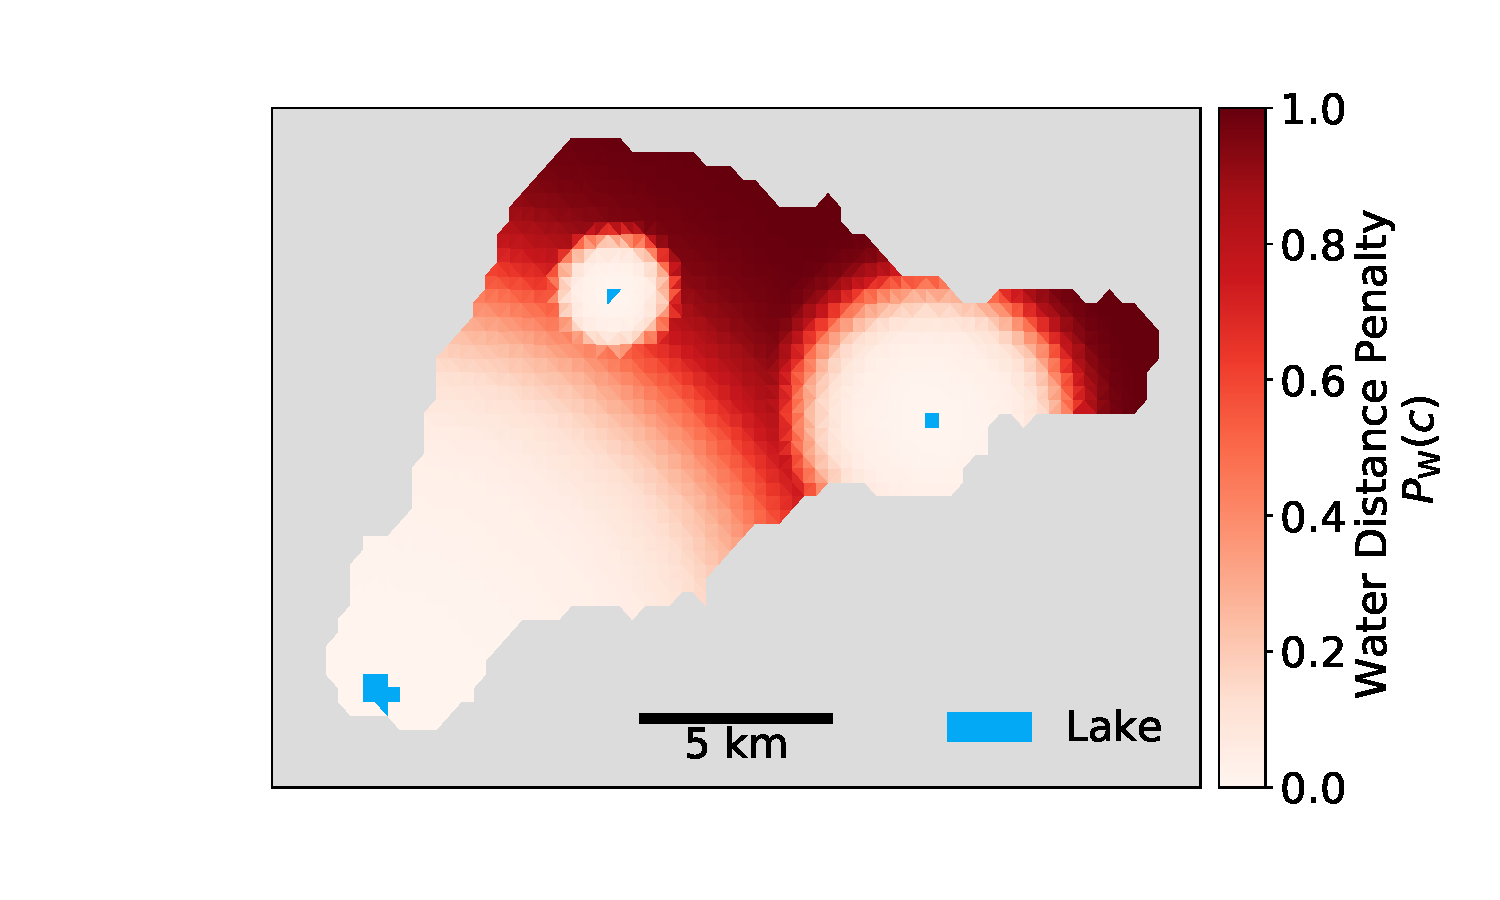
\includegraphics[width=1\linewidth]{images/Plot_PW}
	\caption{The water penalty $P_{\rm W}(c)$ for all cells in times without drought, i.e.\ in which Rano Raraku (in the East) provides freshwater.}
	\label{fig:plotpw}
\end{figure}


%Topic: Elevation Slope
\paragraph{Geographical Constraints}% $P_{\rm G}$
High elevation and slope of Easter Island further penalise the settlement probabilities in this model.
Archaeological evidence (e.g.\ the distribution of the Ahu and Moai) shows that the main settlements remained dominantly within the first $1-2\, \rm{km}$ of the coast, even if upland locations were farmed \citep{Bahn2017}.
There are several possible reasons for that including easier access to small-scale fishing, climatic conditions, or cultural reasons.
Hence, I assume that the geographical penalty depends on a cell's elevation.
While Easter Island is generally quite shallow, especially the North West coast and the areas around the volcano craters are steep, making it difficult for large households to settle in these spots, e.g.\ due to the danger of land slides. 
Hence, the geographical penalty also depends on a cell's slope.
The location evaluation variables, $el(c)$ and $sl(c)$, and the corresponding chosen thresholds $el_{\rm P0.01}=min_{\rm c}(el(c))=0\, {\rm m}$ and $el_{\rm P0.99}=max_{\rm c}(el(c)) = 300\, {\rm m}$ (without any reference) for the elevation and $sl_{\rm P0.01}=0^\circ$ and $sl_{\rm P0.99}=7.5^\circ$ (without any reference) for the slope. 
Then, with corresponding $k_{\rm el}$ and $k_{\rm sl}$ from equation~\ref{eq:k}, the penalties for terrain elevation and slope are calculated as 
\begin{eqnarray}
	P_{\text{el}}(c) = \frac{1}{1+\exp\left( - k_{\rm el} (el(c)-\frac{el_{\rm P0.01}+el_{\rm P0.99}}{2}) \right)}\\
	P_{\text{sl}}(c) = \frac{1}{1+\exp\left( - k_{\rm sl} (sl(c)-\frac{sl_{\rm P0.01}+sl_{\rm P0.99}}{2}) \right)}
\end{eqnarray}
The (combined) geographical penalty $P_{\rm G}$ for a cell $c$ is simply the average of $P_{\rm el}$ and $P_{\rm sl}$:
\begin{equation}
%P_{\rm G}(c) = \rm{max}\left(P_\text{el}(c), P_\text{sl}(c) \right)
P_{\rm G}(c) = \left(P_\text{el}(c)+P_\text{sl}(c) \right)/2
\end{equation}
Figure \ref{fig:P_G} shows the geographic penalty, $P_{\rm G}$, which is constant for all agents and times.
\begin{figure}
	\centering
	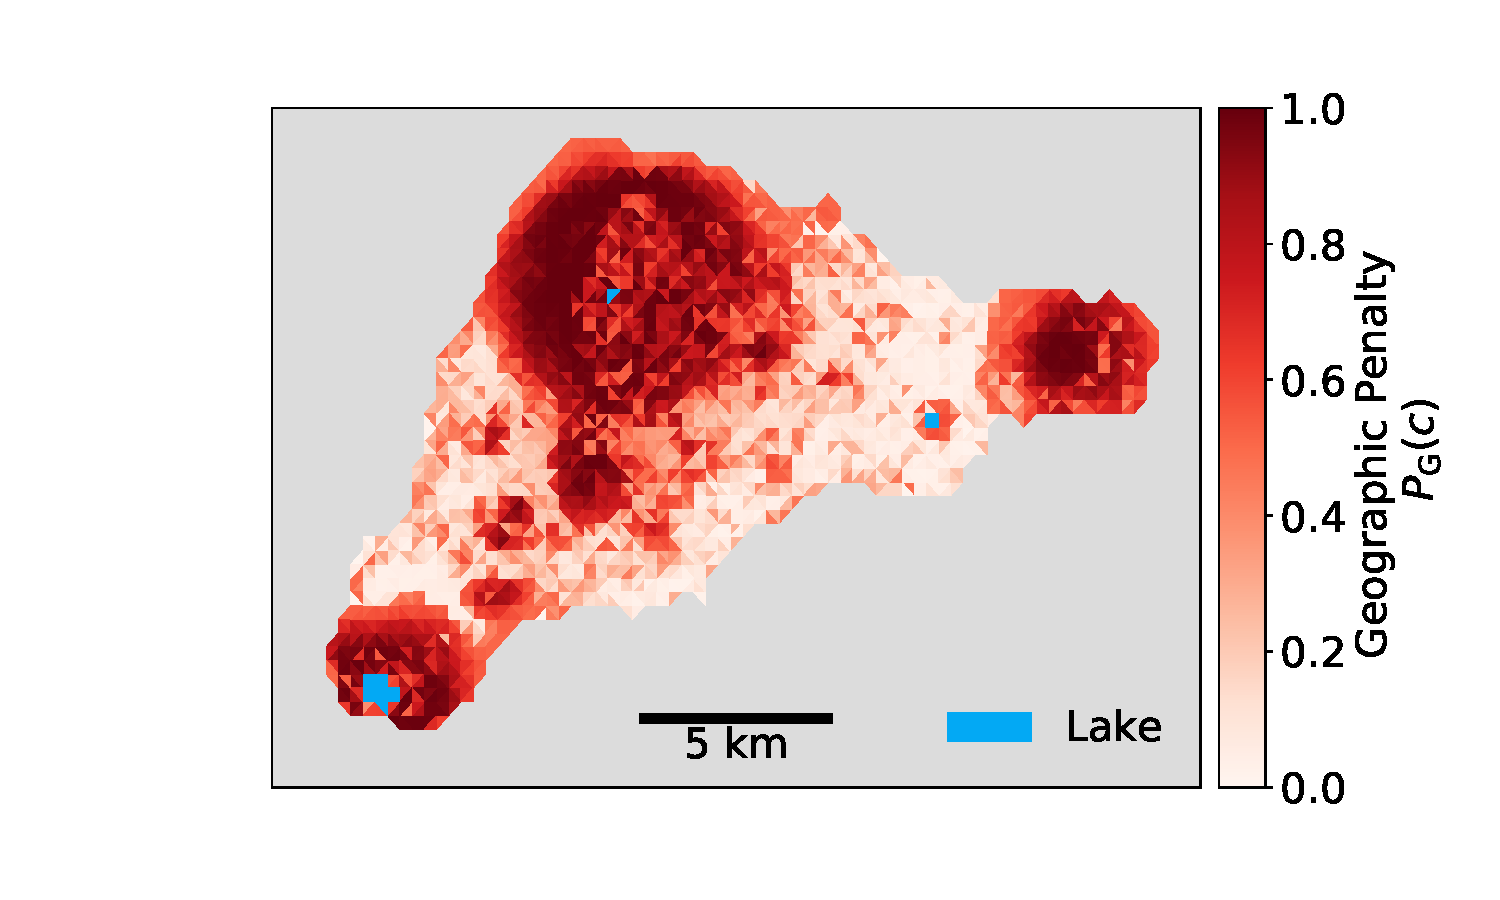
\includegraphics[width=1\linewidth]{images/Plot_PG}
	\caption{The constant geography penalty $P_{\rm G}$ for all cells.}
	\label{fig:P_G}
\end{figure}

% TOPIC: Pop Density Penalty
\paragraph{Population density} % $P_{\rm D}$
Agents also avoid moving to locations with a large population density.
While different agents share the same resources and, thus, interact with the same environment, their actions and moving decisions are independent from each other. 
However, the population penalty by making locations with high population density unfavourable introduces an indirect agent-agent interaction. 
%To some degree, this is incorporated in the farming penalty (later) as well, as regions with large population density, also have fewer available agriculture sites.
I define the population density of a cell as the population density within the farming radius of cell $\tilde{c}$, i.e.\ $C_{\rm F}(\tilde{c})$.
\begin{equation}
pd (\tilde{c}) = \frac{\mathbf{pop}|_{\hat{c} \in C_{\rm F}(\tilde{c}) }}{r_{\rm F}^2 \pi}
\end{equation}
The thresholds are chosen as
\begin{equation}
pd_{\rm P0.01} = 0 \, {\rm \frac{ppl}{km^2}}
\end{equation}
and 
\begin{equation}
pd_{\rm P0.99} = 300 \, {\rm \frac{ppl}{km^2}}
\end{equation}
with \citet{Kirch2010} estimating values of $262$ and $389\, {\rm \frac{ppl}{km^2}}$ (according to \citet{Puleston2017}) on `prime agricultural land' in Hawaii and Maui, which are likely overestimates of the maximum local densities on Easter Island \citep{Puleston2017}. %Puleston state that!!
%The latter is chosen from local population density estimates of \todo{Puleston 558}.
Then, the (time dependent) population density penalty for one cell is
\begin{equation}
P_{\rm D}(\tilde{c}) = \frac{1}{1+\exp\left( - k_{\rm D} (pd(\tilde{c})-\frac{pd_{\rm P0.01} + pd_{\rm P0.99}}{2}) \right)}
\end{equation}
with the corresponding $k_{\rm D}$ calculated from equation~\ref{eq:k}.
		
% TOPIC: Tree Penalty
\paragraph{Availability of Trees} %$P_\text{T}$
Next, scarcity of trees in the local surrounding of a specific location also penalises a possible settlement.
The tree penalty $P_{\rm T}(\tilde{c})$ is determined via the evaluation variable $tr(c)$, the number of trees within $C_{\rm T}(\tilde{c})$,
\begin{equation}
	tr(\hat{c}) = \sum_{\hat{c} \in C_{\rm T}(\tilde{c})}\, T(\tilde{c},t) \ .
\end{equation}
A cell with large value of $tr$ has a lower tree penalty.
There is no intuitive threshold for having a negligible tree penalty, $tr_{\rm P0.01}$ (or optimal number of trees).
Here, I choose this value as the tree number sufficient to fill the tree requirement for a population at a very high population density of $pd = pd_{\rm P0.99}$ in the tree search radius, $C_{\rm T}(c_{\rm i}(t))$, with maximum tree preference $T_\text{Pref, max}$ for roughly one generation ($\sim 45\, {\rm yrs}$).
%a household with population size $42$ (the mean splitting population threshold) and maximum tree preference $T_\text{Pref, max}$ to fill its tree needs for the average lifespan of an individual ($\sim 45\, {\rm yrs}$)
\begin{equation}
tr_{\rm P0.01} = T_\text{Pref, max} \cdot T_\text{Requ, pP} \cdot \left(pd_{\rm P0.99} \cdot \frac{r_{\rm T}^2}{r_{\rm F}^{2}}\right) \, {\rm ppl} \cdot 45\, {\rm yrs} = 
216\cdot 10^3 \, {\rm trees} \ .
\end{equation} 
The threshold, $tr_{\rm P0.99}$, is chosen as the tree number required to keep the current agent's population at a happiness level of at least $h_{\rm i}(t) = H_{equ}$ for the next year:
% $T_\text{Requ, i}(t) \cdot H_\text{equ} \cdot 5\, {\rm yrs} $
\begin{equation}% $T_\text{Requ, i}(t) \cdot H_\text{equ} \cdot 5\, {\rm yrs} $
tr_{\rm P0.99, i}= T_\text{Pref, i}(t) \cdot T_\text{Req, pP} \cdot pop_{\rm i}(t) \cdot H_\text{equ} \ ,
\end{equation}
which is typically between $5-100\, {\rm trees}$ depending on the properties of agent $i$.
On top of the logistic penalty dependency, I further enforce a necessary condition of tree availability at $tr_{\rm P0.99}$: 
A cell $\tilde{c}$ is only considered as viable settlement location if the number of trees at least fulfills $tr(\tilde{c}) \stackrel{!}{\geq} tr_{\rm P0.99}$. 
%in to relocate to a specific cell is set in place (for trees and later also farming):
%To move to a spot in cell $\tilde{c}$, 
%At least sufficient trees to reach $h_{\rm i}(t)\geq H_{\rm equ}$ in the next year have to be present, i.e.\ $tr(\tilde{c}) \stackrel{!}{>} tr_{\rm P0.99}$. Otherwise, penalty is $P_{\rm T}= \infty$ to ensure that the cell is avoided by the agent even if all other penalty contributions are favourable.
In total, 
\begin{equation}
P_{\rm T}(\tilde{c}) = 
\begin{cases} \infty & { if }tr(\tilde{c})< tr_{\rm P0.99} \\
\frac{1}{1+\exp\left( - k_{\rm tr} (tr(\tilde{c})-\frac{tr_{\rm P0.01}+tr_{\rm P0.99}}{2}) \right)} & \text{ else }
\end{cases}
\end{equation}
%Hence, agents favour locations with a large tree density around the cell.


%Unless the agent's population size is reduced or its tree preference changes the agent will have to move in the next year again though. 

%The tree penalty $P_T$ is large if the number of trees in $C_T(\tilde{c})$ around the new location $\tilde{c}$ is much smaller than its maximum on the island:
%\begin{equation}
%	T_\text{reachable}(\tilde{c}) = \sum_{\hat{c} \in C_T(\tilde{c})} \, T(\hat{c}, t)
%\end{equation}
%Again, the scaled $tanh$ function (equation \ref{eq:scaledtanh}) is used relative to the maximum number of possible trees 
%\begin{equation}
%	T_\text{max, reachables} 
%\end{equation}
%of the local number of trees in $C_T(\tilde{c})$ around the new location $\tilde{c}$ is used to derive the tree penalties:
%\begin{equation}
%	P_T = \text{scaledTanh}_T(c,T_\text{50\%P}), T_\text{100\%P}, \kappa)
%\end{equation}
%where the tree 



% TOPIC: Agric Penalty
\paragraph{Availability of Farming Land}%$P_{\rm F}$
%Location penalised by agriculture
Finally, also availability of farming sites influences the agent's moving decision.
The penalty for farming, here, depends on two evaluation variables: 
The total available farming potential $F_\text{tot}(\tilde{c})$ and the available farming potential from non-eroded, well-suited cells only, $F_\text{well}(\tilde{c})$.
The penalties for both variables are calculated separately and then averaged.
The total available farming potential is simply a summation of all productivity indices of arable, unoccupied sites (number of acres within a cell) within $C_\text{F}(\tilde{c})$.
\begin{equation}
	F_\text{tot}(\tilde{c}) = \left( \sum_{\hat{c} \in C_{\rm F}(\tilde{c}) }\, F_{\rm PI}(\hat{c}) \cdot (A_{\rm acres}(\hat{c})  - \mathbf{A}_{\rm F}(\hat{c}, t) )\right) \ ,
\end{equation}
where $A_{\rm acres}(c)$ is the number of acres and $ \mathbf{A}_{\rm F}(c,t)$ is again the number of occupied sites (and, therefore, unavailable to new agents) in cell $c$.
Similarly, the farming potential for well-suited cells only is 
\begin{equation}
	F_\text{well}(\tilde{c}) = \left( \sum_{\hat{c} \in C_{\rm F}(\tilde{c}) \ \cup \ F_{\rm PI}(\hat{c})=1} \, F_{\rm PI}(\hat{c}) \cdot (A_{\rm acres}(\hat{c})  - \mathbf{A}_{\rm F}(\hat{c},t) )\right) \ .
\end{equation}
This $F_\text{well}$ is an important consideration for agents as it makes cells more favourable, if the farming produce can be obtained from a few well-suited rather than a larger number of poorly suited sites, which implies a larger workload required.
The threshold for an optimal location w.r.t.\ farming is the maximum possible land needed to be farmed by an agent with population $42$.
\begin{eqnarray}
F_\text{well, P0.01} & = & F_\text{tot, P0.01} =  (1-T_\text{pref, min})\cdot F_\text{Req, pP} \cdot 42\, {\rm ppl}  \\
& = & 
\begin{cases} 16.8\, {\rm acres}  \text{ (with }F_{\rm PI}(c)=1\text{) for high N fixation scenario} \\  57.1 \, {\rm acres} \text{ (with }F_{\rm PI}(c)=1\text{) for low N fixation scenario} \nonumber
\end{cases} 
\end{eqnarray}
The threshold for penalty $P_{\rm F}(c)=0.99$ is the agent's current farming requirement sufficient to obtain a happiness index of $h_{\rm i}(t) = H_{\rm equ}$, i.e.\
\begin{equation} 
F_\text{well, P0.99, i} = F_\text{tot, P0.99} = (1-T_\text{pref, i}(t))\cdot F_\text{Req, pP}\cdot pop_{\rm i}(t) \cdot H_{equ} \ , 
\end{equation}
which depends on the tree preference and population size.
The parameter, $k_{\rm F}$ is the same for both evaluation variables $F_\text{well} $ and $F_\text{tot}$.
Equivalent to the tree penalty $P_{\rm T}$, a necessary condition for moving to a cell is enforced:
 A cell $\tilde{c}$ is only considered as viable settlement location if the total\footnote{And, hence, also the well-suited} farming potential at least fulfils
 $F_\text{tot}(\tilde{c})  \stackrel{!}{\geq} F_\text{tot, P0.99}$.
 % , for all cells with $Y_\text{tot}(\tilde{c})< A_\text{Req, i}(t) \cdot H_{equ}$ (i.e.\ $a_\text{tot} < a_\text{tot, P0.99}$), the penalty is set to $P_F(\tilde{c})=1$ 
Then, the total penalty is 
\begin{equation}
P_{\rm F} (\tilde{c}) = 
\begin{cases} 
\infty & \text{ if } F_\text{tot} < F_\text{tot, P0.99}\\
\frac{0.5}{1+\exp\left( - k_{\rm F} (F_\text{well}(c)-F_\text{P0.5}) \right)} + \frac{0.5}{1+\exp\left( - k_{\rm F} (F_\text{tot}(c)-F_\text{P0.5}) \right)} & \text{ else}
\end{cases}
\end{equation}
with $F_\text{P0.5} = \frac{F_{\rm P0.01}+F_{\rm P0.99}}{2}$.
In summary, the farming penalty is smallest for those cells surrounded by a lot of well-suited, available sites.
The penalty is large for those cells surrounded by few available, arable sites in general and few available, well-suited sites in particular.
%E.g.\ penalty $P_{\rm F}=0.5$ 
At Anakena Beach, where open-sea fishing is allowed and, therefore, farming not required (if the external restriction $N_{\rm Fisher}(t)<N_\text{Fisher, Max}$ holds), I set the `farming' penalty to a negative value to encourage agents to move there:
\begin{equation}
	P_{\rm F}(\hat{c}) = - 1 %(1-T_\text{Pref, i}(t)) 
	 \quad \forall \  \hat{c} \in C_\text{F}(c_{\rm Anakena}) \text{ if }N_{\rm Fisher}(t)<N_\text{Fisher, Max}
\end{equation}


 \begin{table}
	\centering
	\begin{tabular}{c|c|L|c|c|S}
		$X$ & $x$& Description & $x_{\rm P0.01}$ & $x_{\rm P0.99}$ & Necessary Condition \\ \hline
		W &$w$ & Area weighted distance of cell to lake & $\frac{(0.5\, {\rm km})^2}{r_\text{Raraku}^2\pi}$ & $\frac{(5\, {\rm km})^2}{r_\text{Raraku}^2\pi}$\\
		G & $el$ & Elevation & $0\, {\rm m}$ & $300\, {\rm m}$ & \\
		& $sl$ & Slope & $0^\circ$ & $7.5^\circ$ & \\
		D & $pd$ & Population density within $r_{\rm F}$ & 0 & $300\, {\rm \frac{ppl}{km^2}}$ & \\
		T & $tr$ & Number of trees within $r_{\rm T}$ & $216\cdot 10^3 \, {\rm Trees}$ & $\sim 5-100^* \, {\rm Trees}$ &  at $x_{\rm P0.99}$\\
		F& $F_{\rm tot}$ & Total possible farming produce within $r_{\rm F}$ & $16.8 \, \rm{acres}$  & $\sim 1-13^* \, \rm{acres}$& at $x_{\rm P0.99}$\\
		& $F_{\rm well}$ & Possible farming produce of well-suited sites within $r_{\rm F}$ & -"- & -"- & -"-\\
	\end{tabular}
\caption{The evaluation variable and chosen thresholds for each penalty category.
	Inserting these into the logistic function (equation~\ref{eq:P_X(c)}) gives the penalties in each category:
	$P_{\rm G}$ for geography, $P_{\rm W}$ for freshwater proximity, $P_{\rm D}$ for population density, $P_{\rm T}$ for tree availability, $P_{\rm F}$ for farming land availability.
	Note, that $x_{\rm P0.99}$ for category $T$ and $F$, representing the minimum amount of resources required, depend on the specific agent's properties (denoted by $^*$).
	This value is a further minimum condition for moving to the cell. For the farming penalty, the thresholds are calculated for the high Nitrogen fixation scenario here.
	For $P_{\rm G}$ and $P_{\rm F}$, which have two elevation variables, the mean of the sub penalties gives the corresponding category penalty.
}
\label{tab:x01x09} 
\end{table}


\paragraph{From Penalties to Probability to New Location}
% TOPIC: From Penalty to Pop, and mask, no sites left?
The resulting penalties for a cell $\tilde{c}$ in $C_{\rm M}(c_{\rm i}(t))$ from all categories are linearly combined to obtain a total penalty, which is then converted to a discrete probability $Pr(\tilde{c})$ of moving to this cell.
With (normed) weights $\vec{\alpha}$ (and the agent's tree preference $T_\text{Pref, i}(t)$):
\begin{equation}\label{eq:vecalpha}
\vec{\alpha} = \left(\alpha_{\rm G},  \alpha_{\rm W}, \alpha_{\rm D},  \frac{T_\text{Pref, i}(t)}{\eta_{\rm i}(t)} \cdot \alpha_{\rm T}, \frac{(1-T_\text{Pref, i}(t))}{\eta_{\rm i}(t)} \alpha_{\rm F}\right)
\end{equation} 
where $\eta_{\rm i}(t) = \frac{\alpha_{\rm T} T_\text{Pref, i}+ \alpha_{\rm F} (1-T_\text{Pref, i})}{\alpha_{\rm T}+\alpha_{\rm F}}$ is a normalisation factor to ensure that, $\frac{T_\text{Pref, i}(t)}{\eta_{\rm i}(t)}\cdot \alpha_{\rm T} + \frac{(1-T_\text{Pref, i}(t))}{\eta_{\rm i}(t)} \cdot \alpha_{\rm F} = \alpha_{\rm T}+ \alpha_{\rm F}$ and, therefore, $||\vec{\alpha}||=1$. 
The total penalty is:
\begin{equation}
P_\text{tot, i}(t) =  \begin{cases} \infty & \text{ if } \tilde{c}\notin C_{\rm M}(c_{\rm i}(t))\\
	 \langle \vec{\alpha}{, } \vec{P} \rangle &  \text{ else}
	 \end{cases}
\end{equation}
with $\vec{P} = (P_{\rm G}, P_{\rm W}, P_{\rm D}, P_{\rm T}, P_{\rm F})$.
Finally, 
\begin{equation}
	Pr(\tilde{c})  = \frac{1}{N} \cdot \exp \left( - \gamma \cdot P_{tot}(c) \right) 
\end{equation}
where $N$ is a normalisation and $\gamma$ is a dimensionless scaling factor, which represents the agent's tendency to actually follow the penalty evaluation. 
By increasing $\gamma$, the agent's move more likely to spaces with higher probability (low total penalty). 
E.g.\ for $\gamma$ \ra $\infty$, agents have perfect knowledge of the island's properties and move to the optimal cell with minimal penalty, i.e.\ the decision making is a fully deterministic optimisation process\footnotemark.
\footnotetext{Proof: Consider the relation between $Pr(c_\text{min})$, where $c_\text{min}$ denotes the cell with the minimal penalty $P_{\rm tot, \ min}$, and $Pr(c)$ for all cells $c$. Then, $Pr(c_\text{min})/Pr(c) = \exp(-\gamma P_\text{tot, min})/ \exp(-\gamma P_\text{tot}(c)) = \exp(-\gamma \cdot (P_\text{tot, min}-P_\text{tot}(c)))$. For $\gamma$ \ra $\infty$ this converges to $\delta_{c=c_\text{min}}$.} 
On the other hand, $\gamma=0$ implies that agents move to any new location without consideration of the associated penalties.
By choosing $\gamma$ large, but finite, I set the agents up to make individualistic, semi-rationale choices when moving, but include stochasticity (e.g.\ due to imperfect knowledge) in the decision.
An agent moves to a site based on individual assessment.
However, multiple agents share the same local environment and, thus, can quickly change the penalties of a location (e.g.\ through deforestation). 
Hence, a low penalty at a certain time, does not imply favourable conditions for the future.
%Hence, when agents in this model decide on relocating their settlement, they do not calculate the society's optimal outcome as often assumed in mathematical models (e.g.\ \citet{Good2006}).
%Instead, agents decide by avoiding locations that seem unfavourable based on their knowledge of the current situation.
% choosing a well suited location to surviving and increasing their population size.

Having selected a new cell, the agent chooses a location within this cell with uniform probability
\footnote{Note, that by choosing a location within this cell, the actual availability of arable, free land and/or trees, might deviate slightly from the calculation of the cell's penalty, as the agent's new location (and therefore the definition of the local environment) is not the midpoint as used for the calculation in the moving module).
This accuracy error decreases with a higher discretisation resolution.}
The total procedure of calculating the probability is sketched in Figure \ref{fig:sketchmoving}.

\begin{figure}
	\centering
	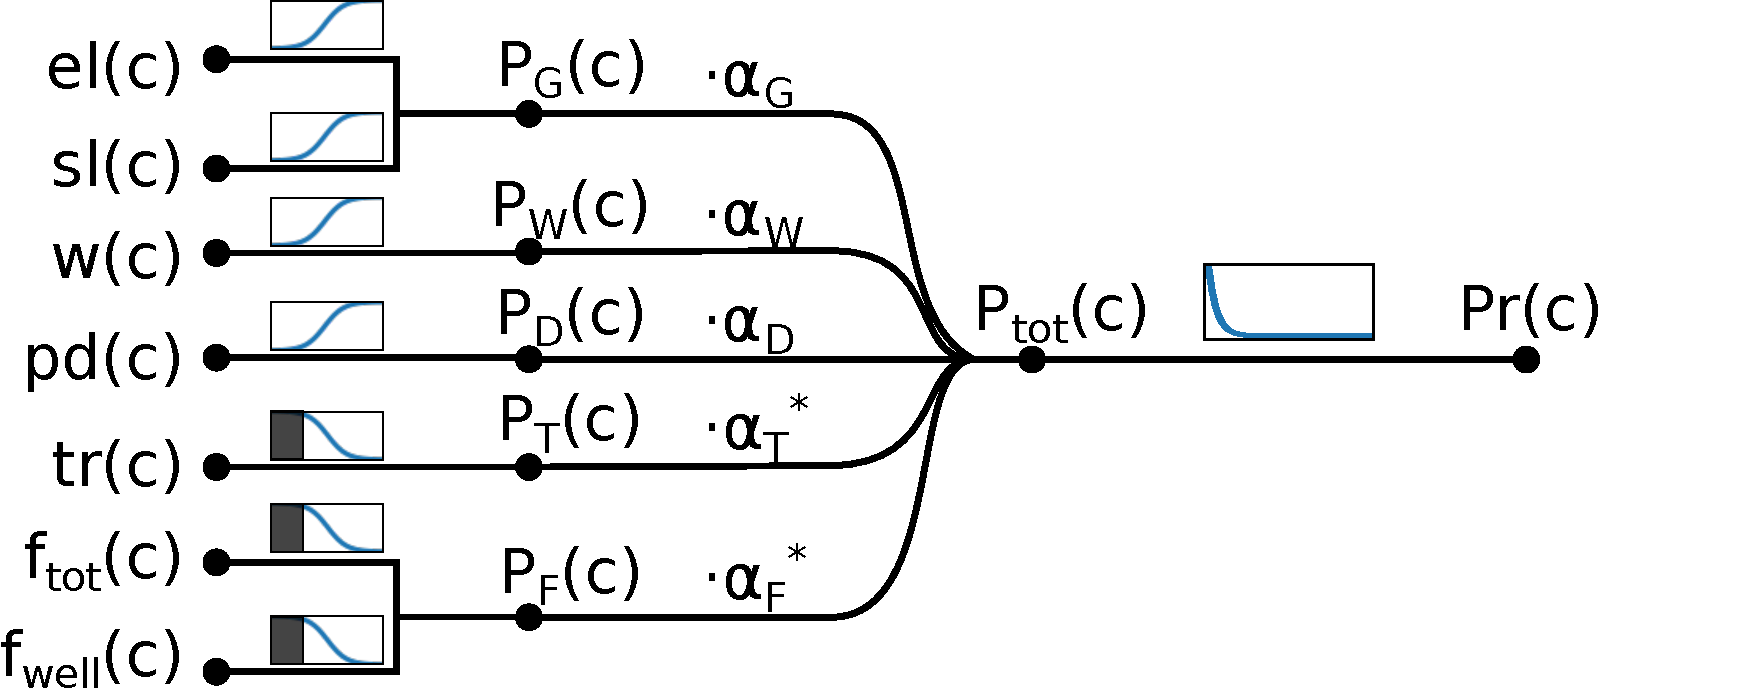
\includegraphics[width=1\textwidth]{images/SketchABM2/sketchMoving}
	\caption{A sketch of the calculation of the probability for agent $i$ to relocate its settlement to cell $c$: The category penalties ($P_{\rm G}$ for geography, $P_{\rm W}$ for freshwater proximity, $P_{\rm D}$ for population density, $P_{\rm T}$ for tree availability, $P_{\rm F}$ for farming land availability) are calculated via one or two characteristic evaluation variables described in the main text assuming a logistic functional dependence (blue curves). 
	If two evaluation criteria are considered for one category, the resulting sub-penalties are averaged (crossings for $P_{\rm G}$ and $P_{\rm F}$).
	For $P_{\rm T}$ and $P_{\rm F}$, cells that do not have the minimum required resource availability are excluded (black boxes).
	The total penalty for cell $c$, $P_{\rm tot}(c)$ is then a linear superposition of all category penalties (with the weights $\alpha_{\rm T}^*$ and $\alpha_{\rm F}^*$ adjusted according to the tree preference $T_{\rm Pref, i}(t)$ (equation \ref{eq:vecalpha}).
	The final probability for a cell $c$ is derived as $Pr(c) \sim e^{-\gamma \cdot P_{\rm tot}(c)}$ (blue line in the right part), with scaling factor $\gamma$.} 
	\label{fig:sketchmoving}
\end{figure}



% TOPIC: When does it occur, calc penalty in each day, \ldots
%With this procedure, agent's move (as resource availability becomes scarce or a subgroup splits from a large household) according to environmental features. 
%The specific settings create spatial patterns of settlement behaviour which in turn non-linearly change the agent-environment interaction and, thus, environment dynamics overall.

\paragraph{Computation Time of the Moving Process}
This evaluation of potential of moving agents is the bottleneck w.r.t.\ computation time in this model.
A single evaluation process scales quartic with the grid resolution $\delta_{\rm x,y}$, i.e.\ $\mathcal{O}(\delta_{\rm x,y}^4)$, the number of grid points per unit length: The overall number of cells to consider $N_{\rm c}$ increases quadratic with $\delta_{\rm x,y}$ and the evaluation of penalties (e.g.\ summing up trees from cells in $C_{\rm T}(\tilde{c})$) for a single cell also scales quadratic with the grid resolution.
In order to increase efficiency, I use dot products and distance matrix computation from the python packages \textit{numpy}\footnote{\citet{numpy}} and \textit{scipy}\footnote{\citet{scipy}}, both implemented in \CC.
In an alternative implementation, one could adjust penalties (or characteristic variables) immediately when the agents interact with the environment, which would scale as $\mathcal{O}(\delta_{\rm x,y}^2\cdot N_{\rm agents}(t)\cdot N_{\rm timesteps})$.
However, since the resolution does not have to be small for this study %, and the number of agents moving over all years is small compared to $N_{\rm c}$ and $N_{\rm timesteps} \cdot N_{\rm agents}$, 
the first implementation is not necessarily slower.
	
		
% Measure Agric Productivity in acres of high quality sites
% Why Wood is a primary resource
% Tree Pref changes quickly
% Mention non-reneqabl etc. earlier.
% Burning not really sure??
% Define SItes(c) as int(area)
% mention arable very early and farmed land
		
















%\section{Analysis, Experiments and Sensitivity Runs}
%\paragraph{Categorisation of Parameters}
%The resulting model has a multitude of parameters, settings and parametrisations often associated with large uncertainties. 
%There are in principle two different kinds of parameter choices described in the following paragraphs and summarised in Table \ref{tab:sensitivity}.

\begin{table}
	\begin{tabular}{l|L|K}
%		Parameter &  Std Run & Fix? & Sensitivity Analysis \\ \hline
%		$t_{\rm arrival}$ & $800\, {\rm A.D.}$ & fix & Mostly only important for timing \\
%		$\mathbf{pop}_{\rm arrival}$ & $40$ & fix & -"- (within reasonable estimates)\\ \hline
%		 $F_\text{ Req, pP}$ & $0.5\, {\rm \frac{acres}{person}}$ & 2 & two different environmental scenarios \citep{Puleston2017}\\
%		 $F_\text{PI, [well, eroded, poor]}$ & $[0.8,\ 0.5,\ 0.1]$ & fix & strong impact (especially poor vs.\ well), estimated from \citet{Louwagie2006} \\
%		 $T_\text{Req, pP}$ & $5\, {\rm \frac{Trees}{person\cdot yr}}$ & 2 & strong impact 
%		 estimate from \citet{Brandt2015}, tested 
		Parameter &  Std Run & Sensitivity Tests \\ \hline
		$t_{\rm arrival}$ & $800\, {\rm A.D.}$ & --\\
		$\mathbf{pop}_{\rm arrival}$ & $40$ & --\\ \hline
		 $F_\text{ Req, pP}$ & $0.5\, {\rm \frac{acres}{person}}$ &  $1.7\, {\rm \frac{acres}{person}}$ \\
		 $F_\text{PI, [well, eroded, poor]}$ & $[0.8,\ 0.5,\ 0.1]$ & -- \\
		 $T_\text{Req, pP}$ & $5\, {\rm \frac{Trees}{person\cdot yr}}$ & $10\, {\rm \frac{Trees}{person\cdot yr}}$  \\
		  $T_\text{Pref, min}$ & $0.2$ & -- \\
		  $T_\text{Pref, max}$ & $0.8$ & --\\
		  $T_\text{Pref, min}|_{\rm fisher}$ & $0.5$ & --\\
		  $N_\text{Fisher, Max}$ & $10$ & -- \\ \hline
		  $\mathbf{T}(t_\text{arrival})$ & $16\cdot10^6$ & -- \\
		  $g_{\rm T}$ & $0$ & $5\%/{\rm yr}$ (with pop up of $0.5\%/{\rm yr}$ of $T(c,t_{\rm arrival})$ if land barren for $10\, {\rm yrs}$) \\
		  \hline
		  $g(H_{\rm i}(t))$ (scale) & $0.1$ & --\\
		  $g(H_{\rm i}(t))$ (shape) & $1.95$ & $3$ \\
		  $g(H_{\rm i}(t)=1)$ & $1.007$ & -- \\ \hline
		   Tree Pattern & uniform density for $el(c)<450{\rm m}$, $sl(c)<10^\circ$ & -- \\ \hline
		  $pop_{\rm min}$ & 6 & --\\
		  $pop_\text{max, mean}$ & 42 & --\\
		  $pop_\text{max, std}$ & 3 & -- \\
		  $pop_{\rm split}$ & 12 & --\\ \hline
		  $r_{\rm F}$ & $1\, {\rm km}$ & $0.5\, {\rm km}$ and $2\, {\rm km}$\\
		  $r_{\rm T}$ & $2\, {\rm km}$ & $1\, {\rm km}$ and $4\, {\rm km}$  \\ \hline 
		  $f_{\rm Tree\  Pref}$ & linear & delayed, faster, logistic\\ \hline 
		  $r_{\rm M}$ & $5\, {\rm km}$ (if $\mathbf{pop}(t)>5000$) & -- \\
		  $x_{\rm P0.01}$ & Table \ref{tab:x01x09} & -- \\
		  $x_{\rm P0.99}$ & Table \ref{tab:x01x09} & -- \\
		  $\vec{\alpha}$ & $\alpha_x=0.2 \ \forall \ x$ & `only resource': $\alpha_{\rm T,F} = 0.5$\\
		  
		  $\gamma$ & $20$ & `Trial\&Error Hopping': $0$, `optimal location': $100$ \\
		  Droughts of Rano Raraku & $800-1200\, {\rm A.D.}$, $1570-1720\, {\rm A.D.}$ & -- \\
	\end{tabular}
	\caption{Choices of parameters for the standard run and sensitivity analysis. %The upper half (separated by double line) mainly determines the aggregated population dynamics, the lower half determines the microscopic behaviour and thus influences mainly the spatial patterns.
	}
	\label{tab:sensitivity}
\end{table}

%\paragraph{Parameters Mainly Influencing the Aggregate Population Size}
%The first category of parameters influences directly the island wide, aggregate population dynamics and peak population because they determine the amount of resource acquisition and availability per agent and the population growth with respect to harvest success (or agent's happiness): 
%\begin{itemize}
%	\item the resource requirements calculated from the constant farming requirement per person $F_\text{ Req, pP}$ in combination with the farming productivity indices $F_\text{PI, [well, eroded, poor]}$, the tree harvest requirement per person $T_\text{Req, pP}$ as well as the values for $T_\text{Pref, min}$, and with a lower importance $T_\text{Pref, max}$, $T_\text{Pref, min}|_{\rm fisher}$ and $N_\text{Fisher, Max}$
%	\item the initial number of trees $\mathbf{T}(t_\text{arrival})$ and (if regeneration is enabled) the tree regeneration parameters, i.e.\ the logistic growth rate $g_{\rm T}$, and pop up properties on barren land 
%	\item the demography model parameters, i.e.\ the shape and scale of the population size growth rate function depending on the harvest success $g(H_{\rm i}(t))$ and the initial population growth rate $g(H_{\rm i}(t)=1)$.
%\end{itemize}
%%These parameters have a direct influence on the dynamics of the aggregated population size and its peak value.
%Furthermore, the parameters $t_{\rm arrival}$ and $\mathbf{pop}_{\rm arrival}$ simply influence the timing of the dynamics.
%The uncertainties associated with these parameters are the main source for the  
%discrepancies between contradictory theories about the history of Easter Island.
%This model presented here does not aim to dispute one theory or the other.
%In fact, the model can re-create the proposed population dynamics by adjusting some of the parameters above.
%Hence, while choosing a standard set of parameters, I also investigate some alternative settings of these parameters (shown in Table \ref{tab:sensitivity}) giving rise to different proposed theories of pre-history population dynamics on Easter Island.
%
%\paragraph{Parameters Mainly Influencing the Spatial Patterns}
%The novel part of this study, however is the spatially explicit component and the stochastic, microscopic acting and decision making of the agents in the model.
%The values of parameters associated with this second category are even less known, but as described in the Introduction, reasonable assumptions on the values and functional dependences of the parameters can be made more naturally on the microscopic than the macroscopic level. The parameters in this category are related to the
%\begin{itemize}
%	\item household size, i.e.\ the maximum and minimum population size  of an agent ($pop_{\rm min}$, $pop_\text{max, mean}$, $pop_\text{max, std}$, $pop_\text{split}$)
%	\item resource search radii ($r_{\rm F}$, $r_{\rm T}$ (in combination with the initial spatial distribution of trees, i.e.\ $T(c,t=t_{\rm arrival})$ for cells $c$)
%	\item shape of the response of the tree preference to the changing local environment
%	\item decision making process when moving, i.e.\ the restricted moving radius $r_{\rm M}$, penalty categories and their logistic dependency specified by the thresholds $x_{\rm P0.01}$ and $x_{\rm P0.99}$, the weights $\vec{\alpha}$, and the scale parameter $\gamma$.
%\end{itemize}
%
%% Every Run is a realisation: 
%\paragraph{Analysis}
%Throughout the thesis, I have defined parameter setting for a standard run (details in Table \ref{tab:sensitivity}).
%I perform several sensitivity simulations (also described in Table \ref{tab:sensitivity}) and analyse the corresponding changes to this standard run in both categories of parameters related to the aggregate population dynamics and to the spatial patterns.
%Since multiple processes in the model are stochastic, each run is only a single realisation. 
%While the aggregated results do not differ much between runs with the same setting, the spatial pattern of deforestation varies in general. 
%I perform several ensemble runs, but there is no obvious way to obtain an aggregate spatial mean dynamics per se.
%Instead, variation in spatial patterns for the same experiment are described qualitatively in most cases and by defining distinct spatial regions and looking at their population dynamics separately. 
%
%% Standard Run with table and then Average and Std
%\paragraph{Standard Run and Experiments}

% Perform sensitivity analysis of second for different settings of first categories.

% From standard run, try different moving probabilities.



% !TEX root=frame_thesis.tex
\chapter{Results and Discussion}\label{chapter:Results}
\FloatBarrier
\section{A Standard Configuration Run}\label{sec:std} 
\paragraph{Overview of the Results.}
The standard configuration run results of the ABM presented in Section \ref{chapter:Methods} are produced with parameters presented in Table \ref{tab:sensitivity}.
Figure \ref{fig:STDrull} presents snapshots of a simulation showing the spatial pattern of trees, farmed sites, and agents (with their tree preferences) at different times.
In the supplementary material, I provide a link to an animated Figure showing the evolution of these spatial patterns over time.
Since multiple processes in the model are stochastic, each run with a specific seed is a unique realisation.
In order to obtain statistically valid aggregate results, I use an ensemble of $15$ runs for all experiments.
Adding more runs (e.g.\ 20 or 25) does not significantly change the coefficient of variation for the ensemble over time (see Figure \ref{fig:coeffofvariation}).
The mean and standard deviation of the aggregated variables of this ensemble and their change over time is shown in Figure \ref{fig:STDstats}.
The uncertainty in the ensemble runs results from slight differences in the timing of the dynamics due to different realisations of the discrete, stochastic population growth process (see also Figure \ref{fig:realisationsofpopgrowth}). 
Hence, the peaks of the population sizes of single runs are at a similar level but slightly shifted in time. 
However, due to this shift the resulting ensemble mean (thick line in Figure \ref{fig:STDstats}) slightly underestimates the peak population size.

\begin{figure}
	\centering
	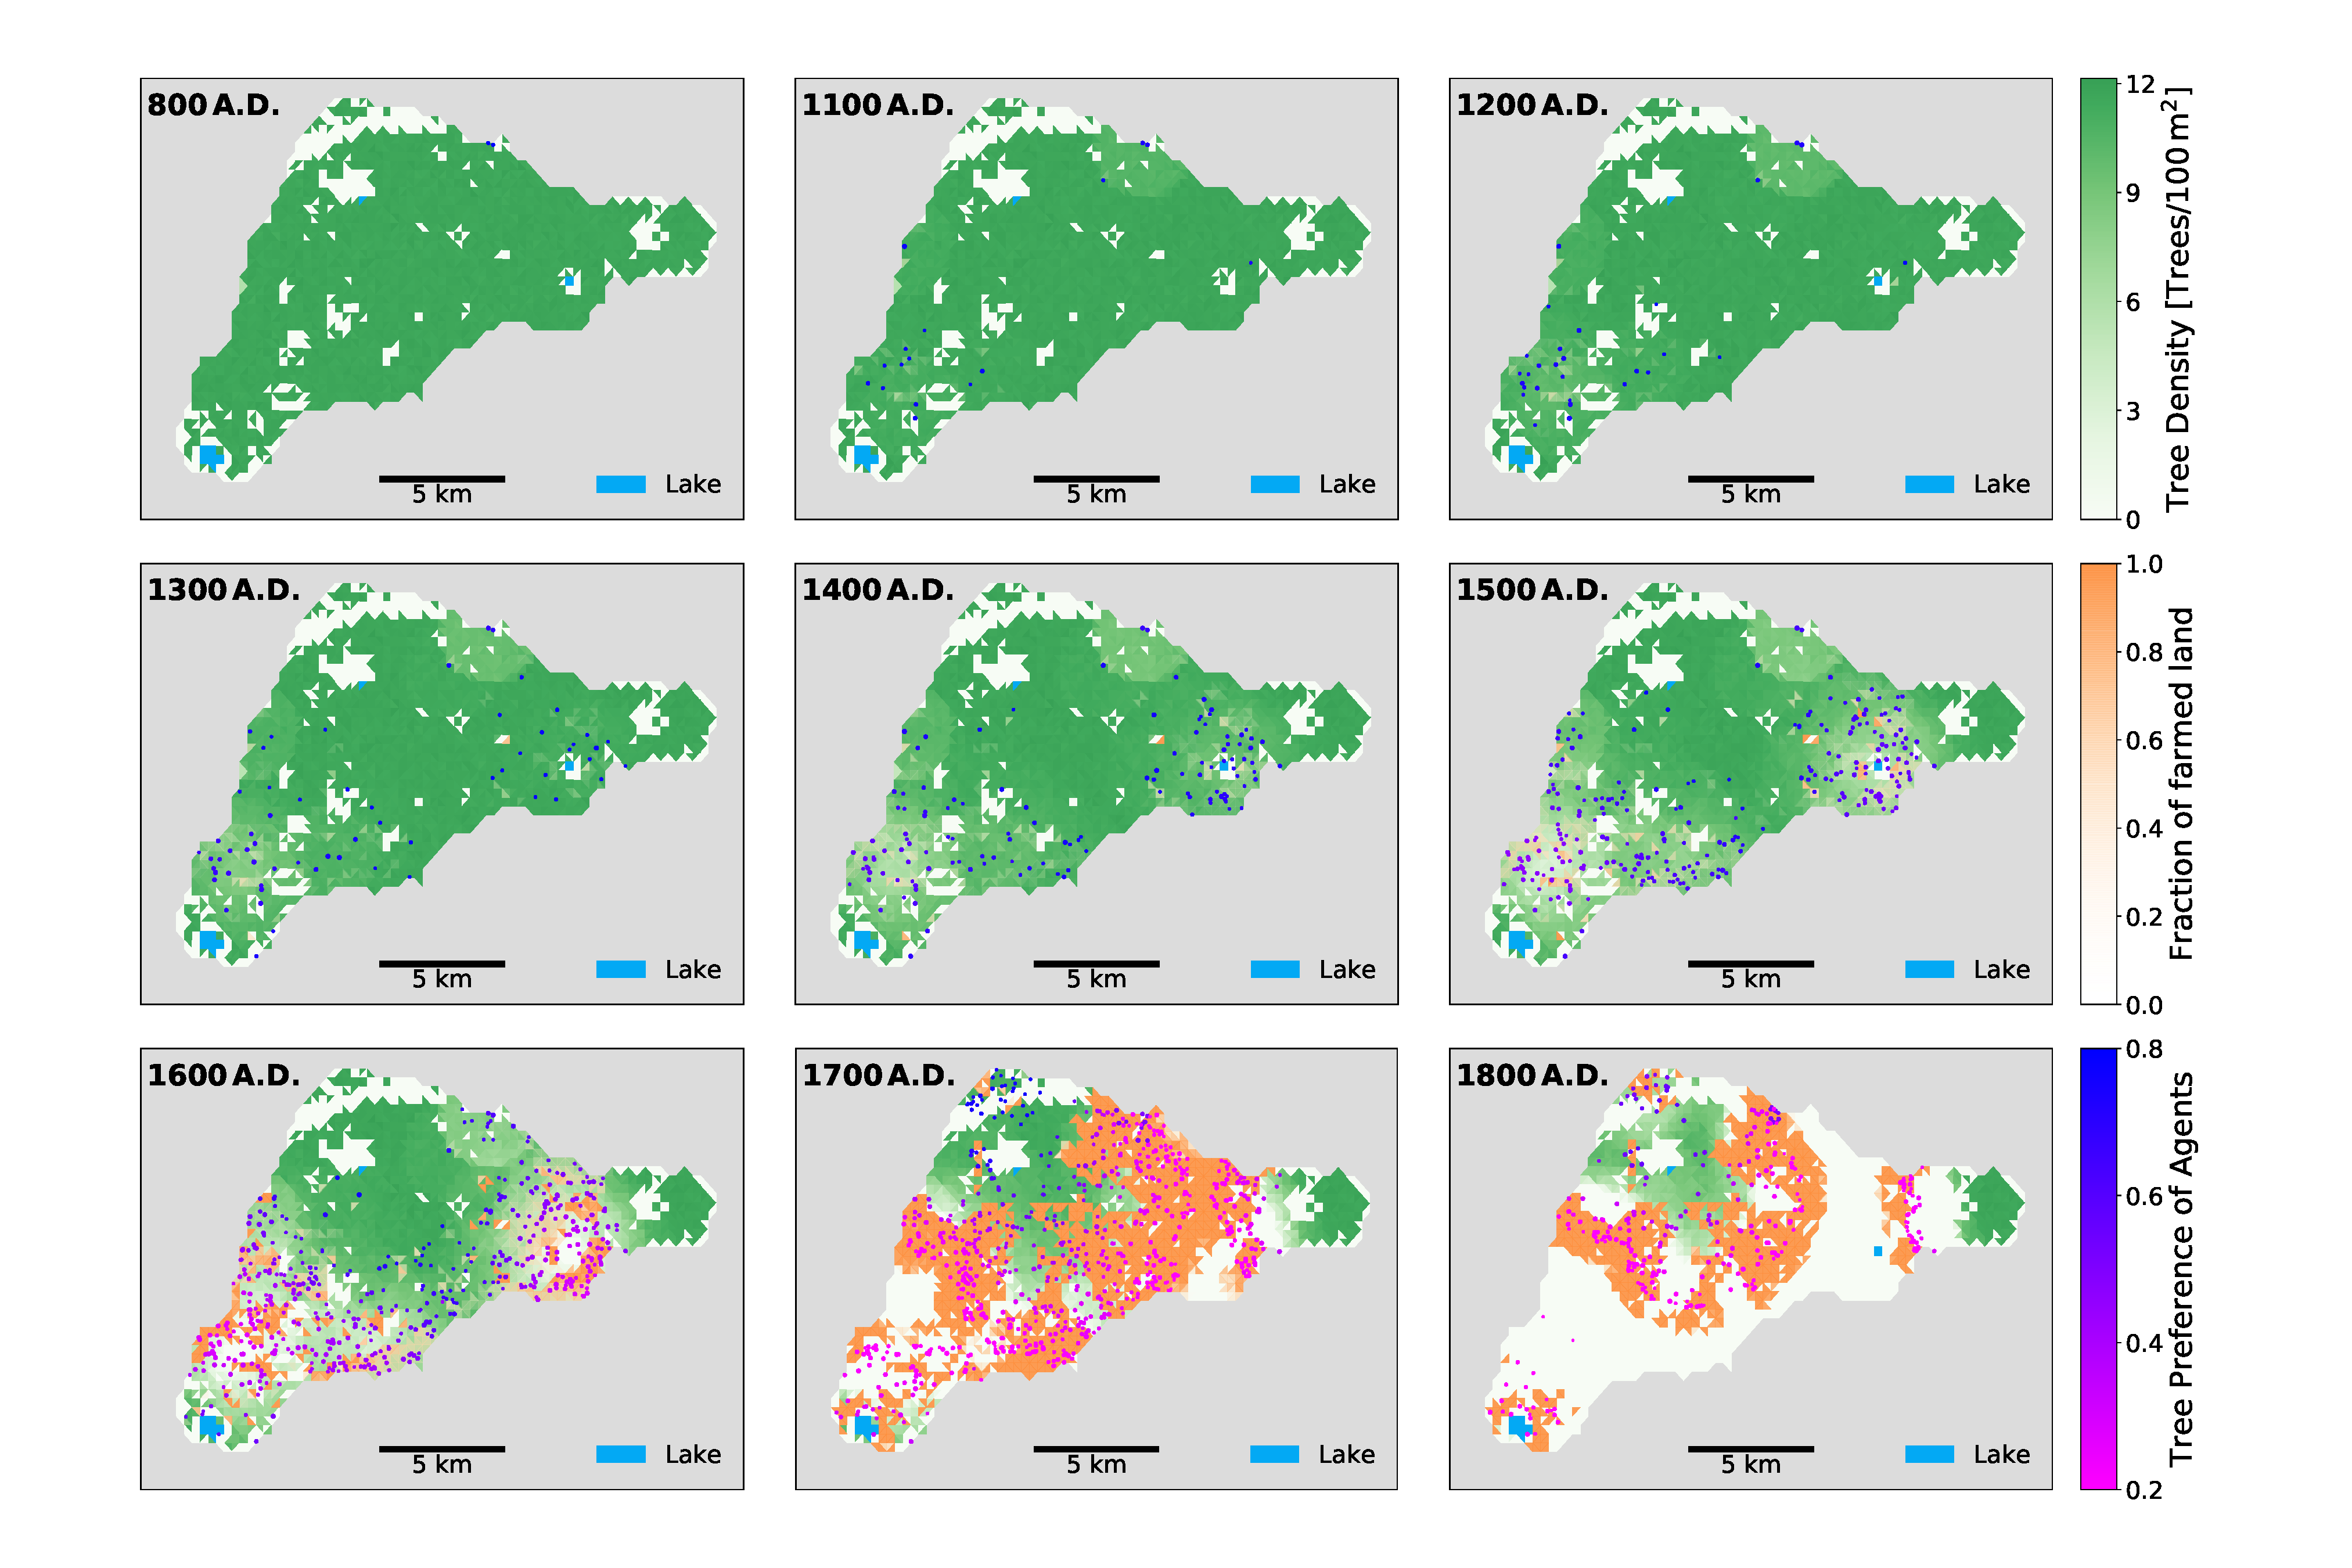
\includegraphics[width=1.3\textwidth, center]{images/Results/Standard/Rull2020_Comparison_seed3}
	\caption{Spatial patterns produced by the ABM in the standard run configuration at nine different times (comparable to Figure 9 in \citen{Rull2020}). The map shows the tree density in green and the fraction of farmed land in orange. Agents are represented by dots with a colour corresponding to their tree preference and size corresponding to their population size. They settle on the island and interact with the environment by cutting trees and turning arable land into farmed sites.}
	\label{fig:STDrull}
\end{figure}


\begin{figure}
	\centering
	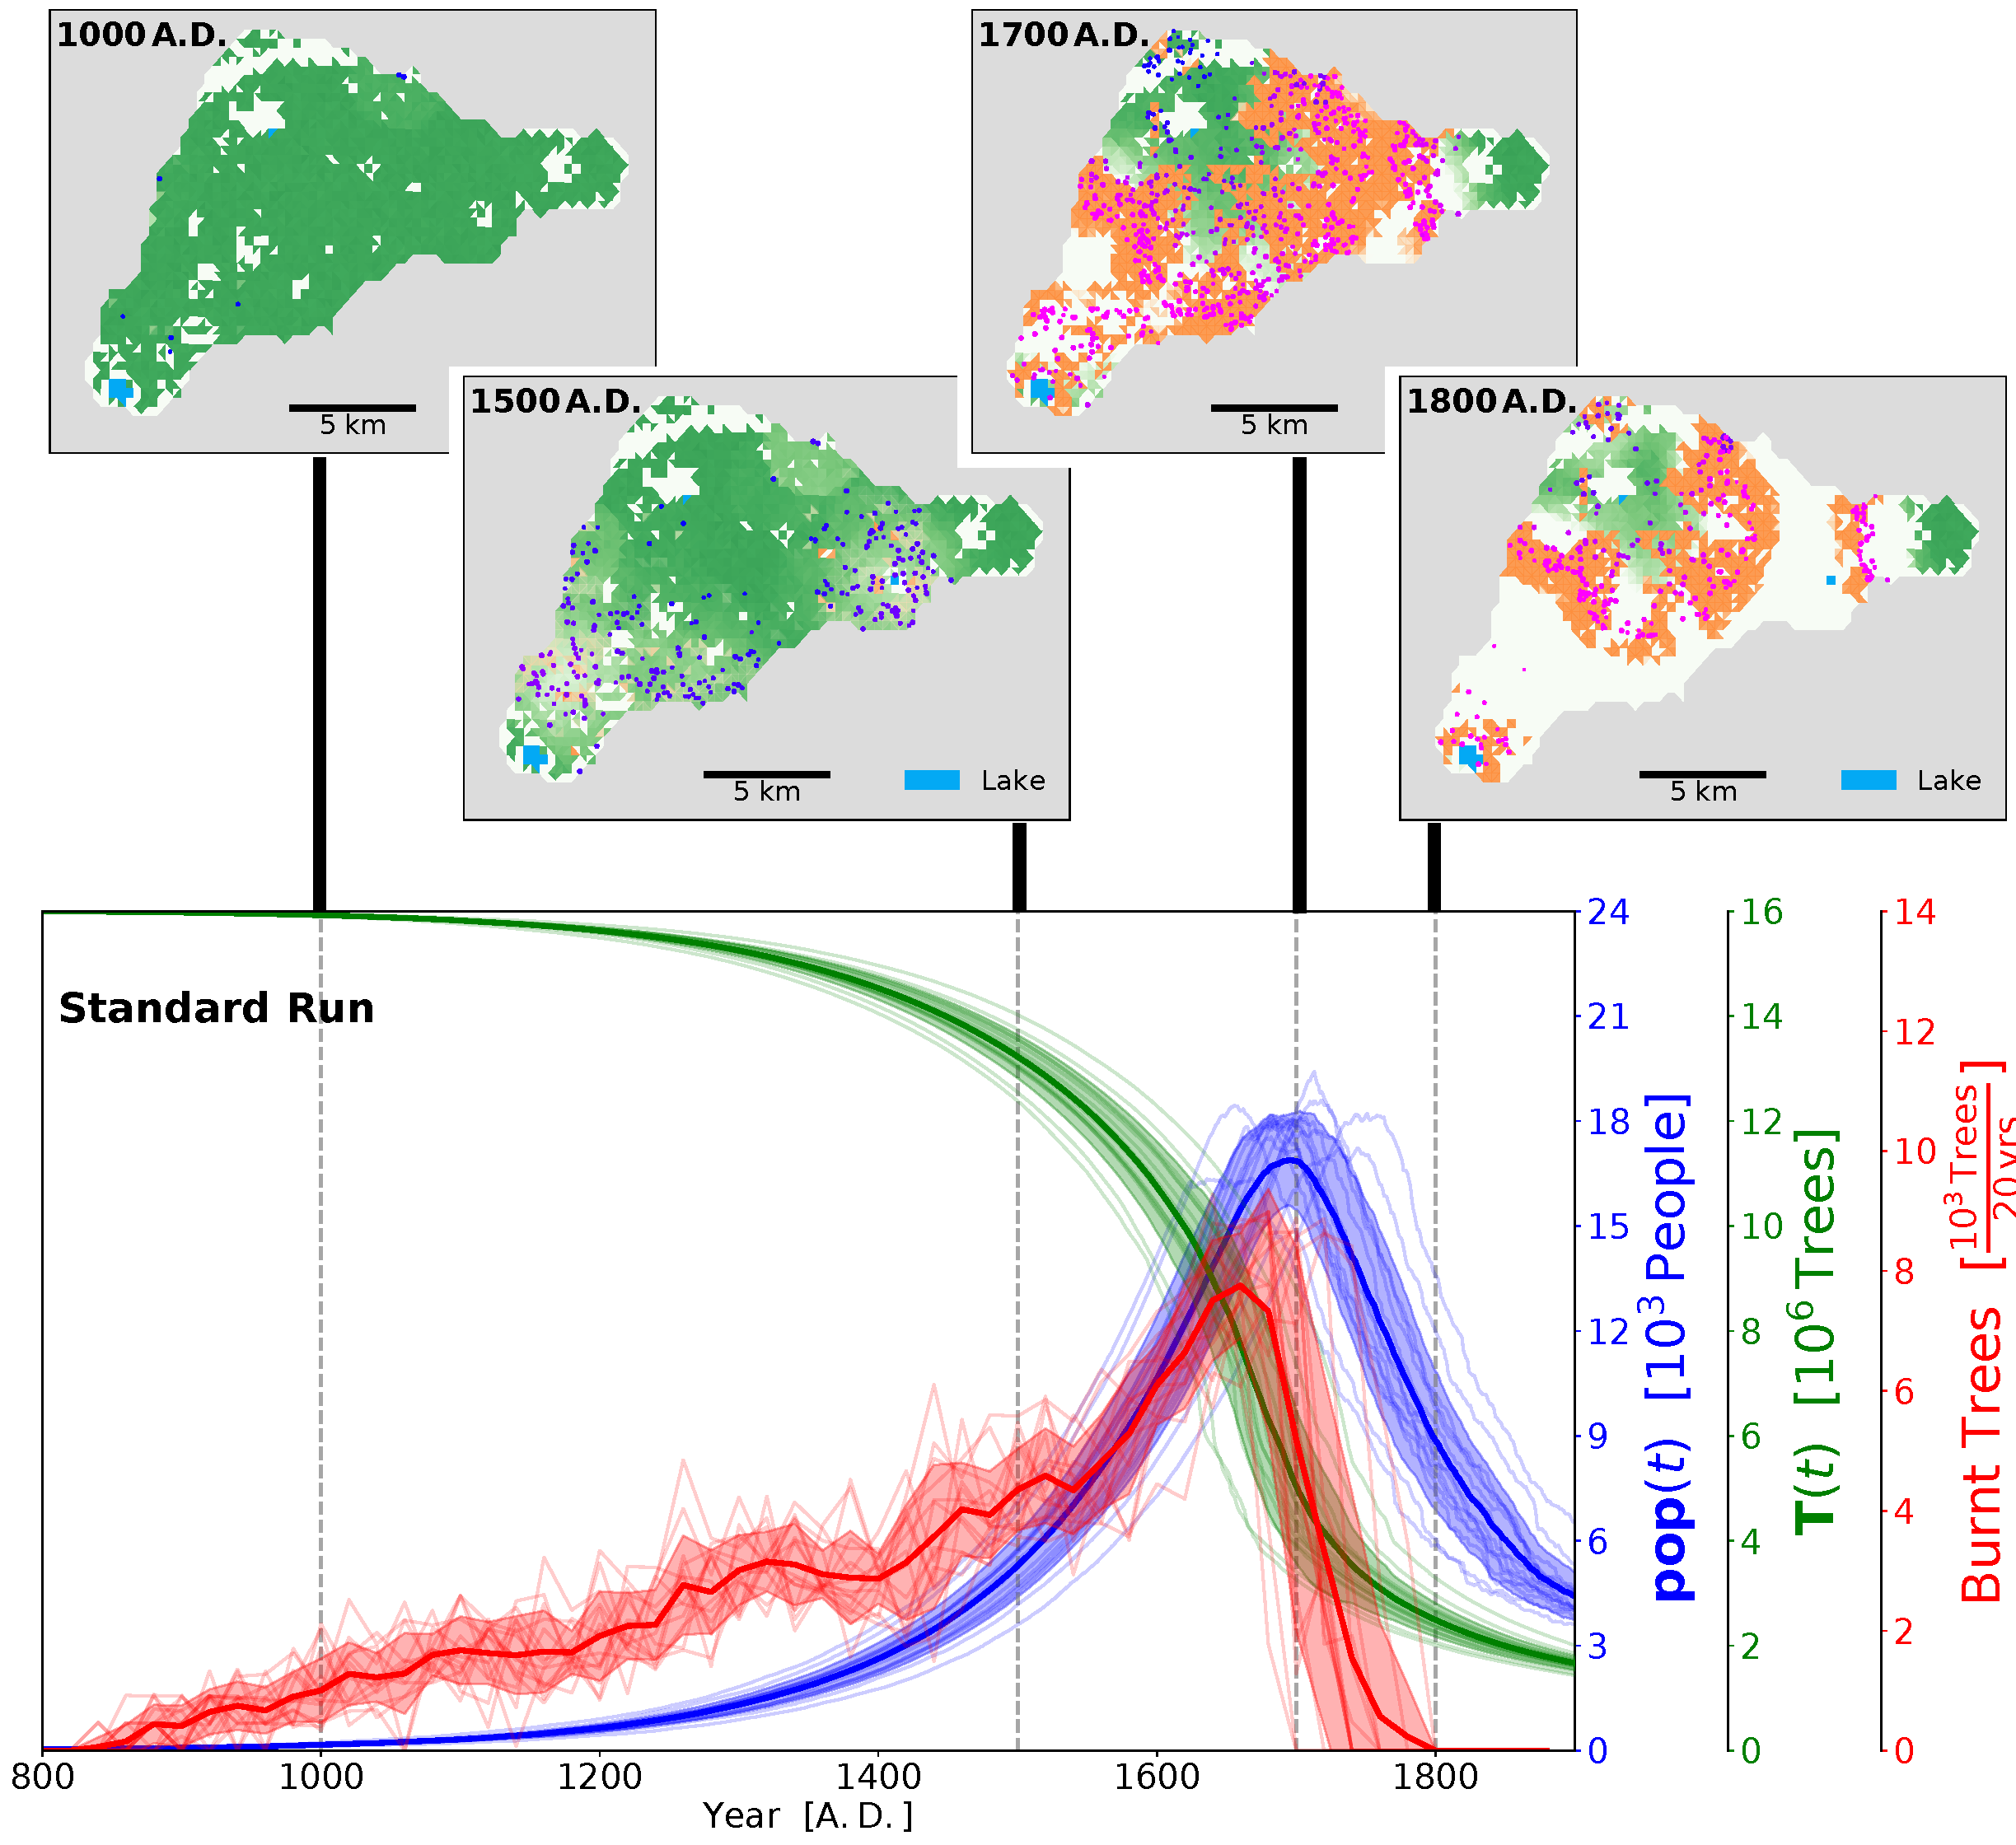
\includegraphics[width=1.\linewidth, center]{images/Results/Standard/EnsembleStatistics+Panels}
	\caption{
		Dynamics of aggregate population size, trees, and burnt trees in the standard run configuration. 15 different realisations (thin lines) are used to obtain the ensemble means (thick lines) and standard deviations (shaded areas). 
		The number of burnt trees is presented in bins of 20 years, as its variation is strong.
		The maps above show the spatial distribution of trees, farming and agent settlements with their tree preferences for one of these realisations (with the same colour coding as in Figure \ref{fig:STDrull}).}
	\label{fig:STDstats}
\end{figure}


\paragraph{The first phase: Initial Growth.}
In the beginning of the simulation, two agents with 20 individuals each settle at Anakena Beach (in the North in Figure \ref{fig:Karte}). 
The local tree density is at the carrying capacity (in total $16\cdot 10^6$ trees) and, thus, the agents' tree preference is high (blue colour in Figure \ref{fig:STDrull}).
In the first phase of the simulated time period, the agents' population size grows at a constant maximum growth rate, because trees and arable land are both abundant. 
Consequently, the number of agents increases and new agents start to colonise the rest of the island. 
Until the end of the first drought period in $1200\, {\rm A.D.}$, new agents tend to settle in the arable, coastal region South/South East of the island close to the major freshwater source Rano Kau. 
After $1200\, {\rm A.D.}$, also the region around Rano Raraku (in the West), now providing an alternative, low elevation freshwater source, is settled at rapid pace.
Agents linearly adapt their tree preference to the slow environmental change and, thus, intensify farming activity.
As Figure \ref{fig:STDstats} shows, the amount of burnt trees to clear land for agriculture also increases linearly in this phase.

\begin{figure}
	\centering
	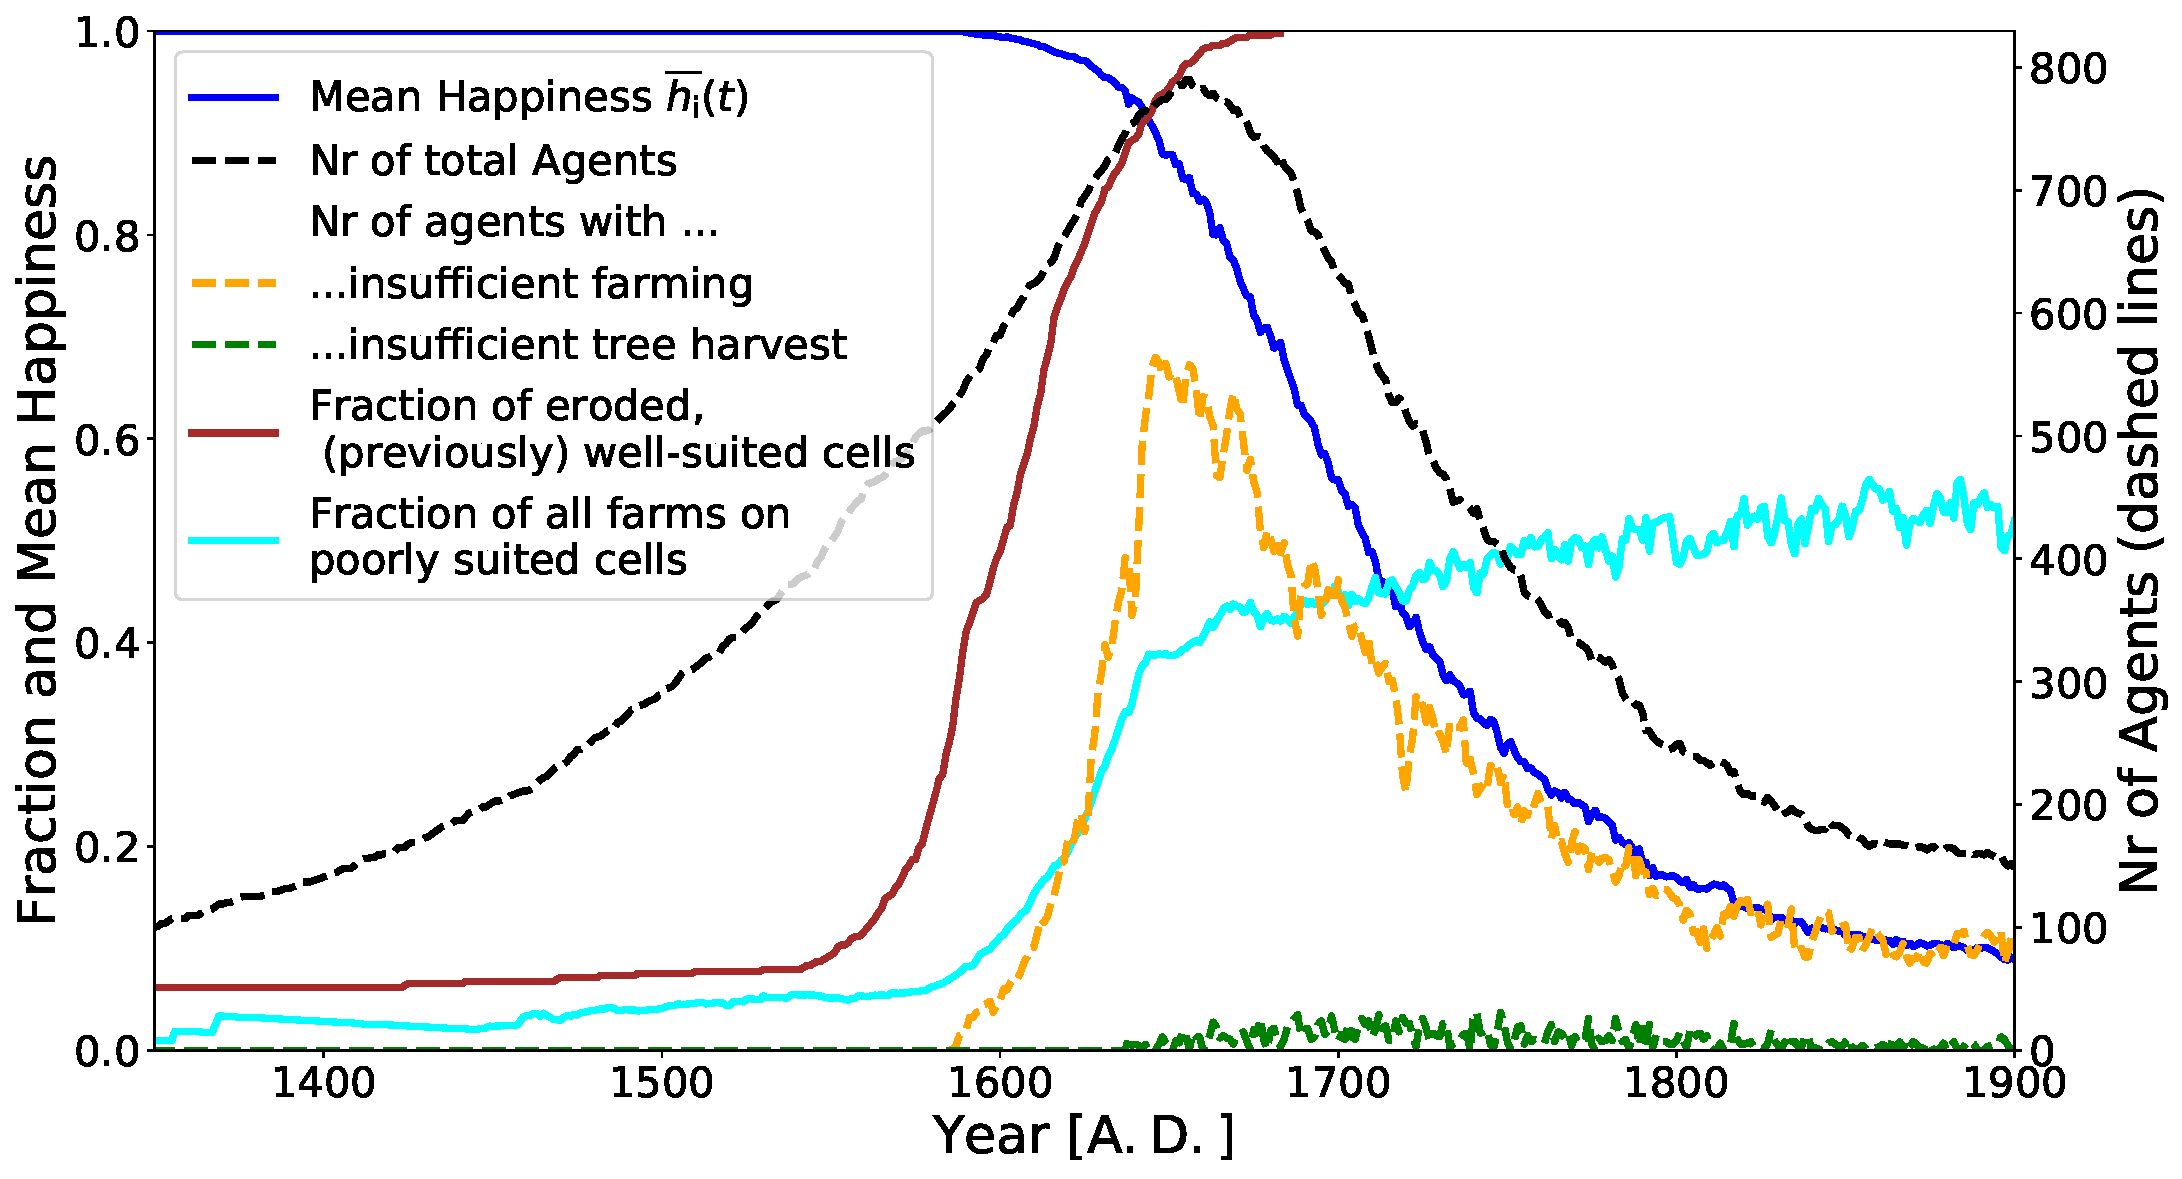
\includegraphics[width=\textwidth]{images/Results/Standard/StandardsecondaryStats}
	\caption{
		Indicators of the change from net growth to net decline in population dynamics for one single realisation in the standard run configuration.
	Dashed lines correspond to the y-axis on the right representing absolute number of agents.
	The blue line shows the mean happiness index of all agents. The black, dashed line shows the total number of agents. The number of agents that lack either sufficient land for farming or trees are shown in yellow and green, respectively. The brown line shows the fraction of cells (previously classified as well-suited for farming) with erosion due to complete deforestation. The cyan line shows the fraction of farming sites on poorly suited sites.}
	\label{fig:STDsecondayrstats}
\end{figure}

%Thereby, agents accelerate the depletion of the non-renewable resource, trees and, thus, in a self-enhancing loop, acquire more farming land.

%Further, this large-scale deforestation leads to a sharp increase of erosion of well-suited sites around $1650\, {\rm A.D.}$ and, hence, agents can not fill their farming requirements.

% with the first agents not meeting their resource requirements.
%However, since both neither further arable sites are available in the densely populated coastal regions and trees are deforested entirely by the remaining agents, these previously well-suited settlement locations are abandoned and the agents turn to the mostly poorly suited upland areas causing a shift towards the interior of the island.
%With the first agents not meeting their farming requirements around 1650, occupation of upland poorly suited farming sites jumps from a negligible fraction in $1650$ to $40-59\%$ in 1700.
%Consequently, the amount of burned trees rises quickly and comes to a abrupt halt between 1700 and 1800.
%Due to the low productivity indices of these sites, the use of burning trees to clear more space rises sharply in this period.

\paragraph{The second phase: Acceleration.}
The second phase of the dynamics is characterised by accelerating, non-linear feedbacks as shown by several indicators (Figure \ref{fig:STDsecondayrstats}).
In a self-enhancing loop, population growth in the settlement centres leads to an intensification of deforestation, a consequent decrease of the agents' tree preferences, increase of farming requirements, more acquisition of farming sites (therefore, more burnt trees) and, thus, more intense deforestation.
Simultaneously, erosion accelerates the deforestation as the farming productivity of occupied land decreases and  more land needs to be acquired.
%of arable farming land increases, leading to declined farming efficiency and, thus, more farming sites required per agent.
The portion of eroded, previously well-suited cells jumps from less than $10\%$ of all well-suited sites in $1600\,{\rm A.D.}$ to $100\%$ by $1700\, {\rm A.D.}$ (brown curve in Figure \ref{fig:STDsecondayrstats}).
Consequently, the amount of trees burnt for clearing land rises sharply. %to roughly $8\cdot 10^3$ trees per $20 \, {\rm yrs}$.
In total, this acceleration of local resource use, leads to an abandonment of the previously used well-suited locations (constituting nearly $100\%$ of all farming activity in $1650\,{\rm A.D.}$) and to the colonisation of mostly poorly suited, interior, upland areas (accounting for $40\%$ in $1700\,{\rm A.D.}$, cyan line in Figure \ref{fig:STDsecondayrstats}).
%The share of farming activity on those poorly suited cells rises from a negligible fraction in $1650\, {\rm A.D.}$ to $40\%$ of all farming activity in $1700\,{\rm A.D.}$ (cyan line in Figure \ref{fig:STDsecondayrstats}).
%However, there is no year in which all available farming sites are occupied simultaneously.
%However, the lower productivity indices in the poorly suited sites, leads to a further increase in land acquisition and, thus, deforestation. 

\paragraph{The third phase: Population Decrease.}
The third phase is characterised by a population decline and a substantial shift in the settlement patterns.
While in $1700\,{\rm A.D.}$ more than half of the agents experience some minor shortage in farming products (yellow curve in Figure \ref{fig:STDsecondayrstats}), 
%there is no time when all arable spaces are farmed simultaneously.
the loss of the trees, experienced by a few agents each year (green line in Figure \ref{fig:STDsecondayrstats}) triggers an exponential decline in averaged happiness, $\overline{h_{\rm i}(t)}$, just after $1700\, {\rm A.D.}$ (blue line in Figure \ref{fig:STDsecondayrstats}).
This leads to a period of intense moving.
Figure \ref{fig:penaltiesag500t1603} shows examples of an agent's penalties while searching for a new settlement location.
\begin{figure}
	\centering
	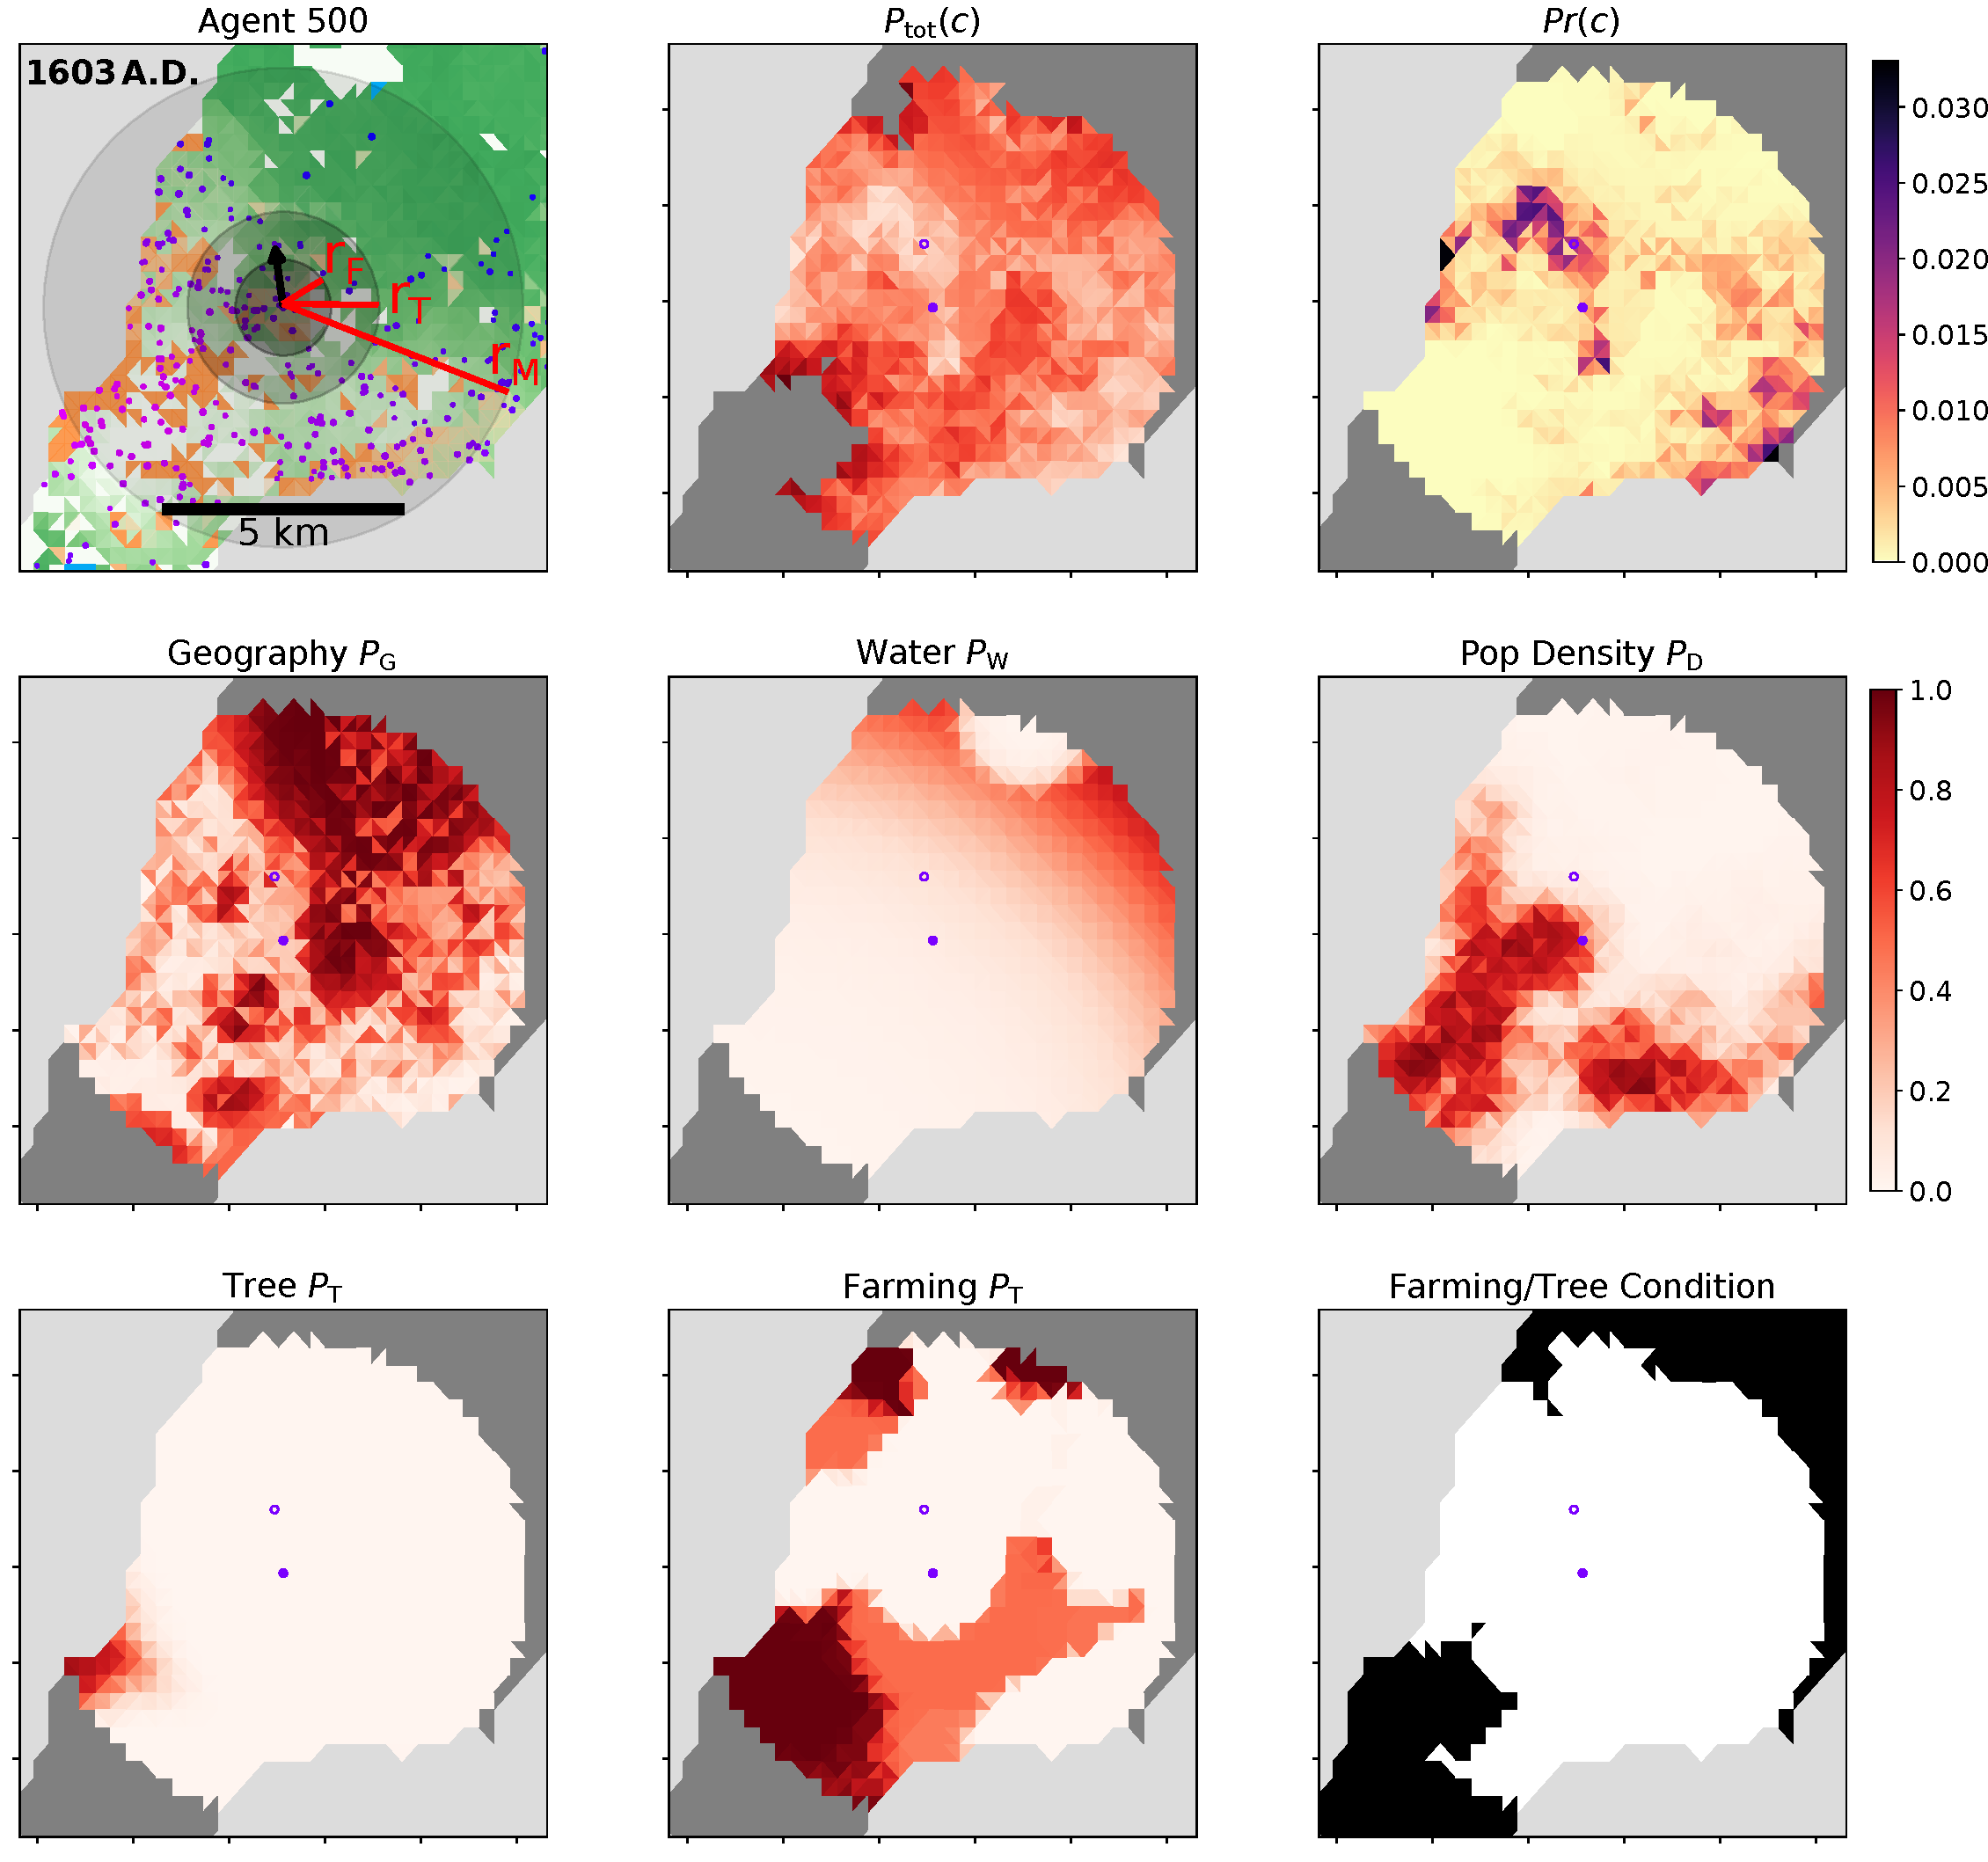
\includegraphics[width=1.3\linewidth, center]{images/Results/Standard/Penalties_AG500_t=1603_rad}
	\caption{Decision making in the moving module of an agent at time $1603\, {\rm A.D.}$ in the South Eastern portion of the island. 
		Each panel shows the same region of interest with the location of the agent in the centre (filled dot) and the new location after the decision is made (unfilled dot).
		The upper left panel shows the agent in its current local environment, indicated by circles with the radii $r_{\rm F}$, $r_{\rm T}$, and $r_{\rm M}$ (after the moving restriction). The upper middle panel shows the total penalty ($\in [0,1]\cup \infty$), and upper right the corresponding probability for the agent to move to each allowed cell. The remaining panels show the penalties in all categories ranging from $0$ to $1$.
		The lower right panel also shows the cells that are excluded from the search because they do not fulfil the necessary condition for tree and farming availability (black cells inside the $r_{\rm M}$ circle).}
	\label{fig:penaltiesag500t1603}
\end{figure}
This phase marks the end of net exponential growth for the population, which peaks at around $18\cdot 10^3$ people around $1700\, {\rm A.D.}$.
Within a relative short time period of less than $50$ years, the population starts to decrease exponentially with a growth rate of $-0.5$ to $-1\%$ (see Figure \ref{fig:app:STDnetgrowthrate} in the Appendix).
The population decreases despite the fact that there are always both unoccupied farming sites and sufficient total number of trees on the island.
However, since the harvest is confined to the local surrounding of an agent in a specific location, it typically lacks one or the other resource and at some point there are no suitable locations left that fulfil both resource requirements.
Consequently, an agent's effective happiness, $H_{\rm i}(t)$ quickly drops to $0$ and the overall population size decreases.
As a result of the decreasing population size, the deforestation level slows down around $1750\, {\rm A.D.}$ at slightly less than $25\%$ of the initial total number of trees. 
%have not enough farming sites with a happiness $H_{\rm i}(t)>H_{\rm equ}$ and therefore positive net growth. 
%The agents unable to find enough trees to cut, however, at this point of time quickly vanish as there are no valid locations to settle anymore and no replacement leading to a memory happiness of $H_{\rm i}(t) = 0$ very quickly.
%Finally, by $1800\,{\rm A.D.}$, the population decrease slows down. 
%The net population growth is shown in Figure \ref{fig:app:STDnetgrowthrate}. 
However, there is no stable coexistence of population and trees in this standard run configuration as tree regeneration is disabled and, hence, the agents rely on a non-renewable resource and, eventually, all agents vanish as it becomes exhausted.


\paragraph{Outcomes Consistent with Ecocidal View.}
The succession of events in the standard run configuration follows a boom and bust scenario consistent with the classical narrative of a Malthusian catastrophe driven by overexploitation as theorised by \citet{Brander1998}, \citet{Diamond2011} and \citet{Bahn2017}.
This is not surprising as the agents are designed to maximise their personal population growth every year while they rely (in the standard run configuration) on a non-renewable resource (trees) and a limited, renewable resource (farming products).
Furthermore, the arrival date and initial population growth are taken from the ecocidal narrative.


\paragraph{Population Size is Maximised Myopically by Model Design.}
In general, the population size reached with this model is at the upper range of most estimates reported in the literature \citep{Bahn2017}.
This is partly due to the fact, that there is no restriction on the amount of labour that agents can put into the resource acquisition. 
Also, the model does not include any social development or political institution e.g.\ to stabilise the population growth or harvest of natural resources via taboos.
Further, I assume that except for the eventual erosion of all well-suited cells, arable land has a constant, entirely predictable crop output (which I assume constant even during drought periods). 
Land availability is, thus, the only constraint for agricultural production in this model configuration. 
%\todo{A certain stochastic variation due to different climatic conditions each year could be implemented into the model.}
Sustainability criteria concerning the resource availability (locally and island-wide) do not play a role in the agents' myopic, unabated population expansion as long as the resource situation allows it.
In addition, agents do not plan ahead while harvesting e.g.\ trees could be cut first (e.g.\ for extracting the sugary sap) and then burned to clear land for farming in the following year as suggested by \citet{Mieth2015}.
Only when resources become scarce, the population growth declines and turns negative.
The pronounced consequent decrease in population size is, thus, inevitable as agents are determined to overexploit.

\paragraph{The Spatial Component.}
This modelling work investigates for the first time spatial component of the Easter Island settlement history emerging from the local harvest behaviour and moving decisions of autonomous agents.
The results (in terms of tree densities and temporal and spatial distributions, Figure \ref{fig:STDrull}) show good agreement with a qualitative reconstruction of tree density obtained from charcoal and pollen data by \citet{Rull2020} (Figures 7 and 9 in the cited literature).
The spatial Easter Island settlement history produced by the model is also mostly consistent with a qualitative colonisation pattern suggested by \citet{Bahn2017} based on archaeological evidence.
This qualitative pattern proposed by \citet{Bahn2017} is as follows.
Settlement of some coastal regions, especially South East Coast near Rano Kau and Anakena Beach ($800$ to $1100\, {\rm A.D.}$), settlement of the whole coast ($1100-1425\,{\rm A.D.}$, with a rapid population increase in the South Coast around $1300\, {\rm A.D.}$), a peak of the population size and farming activity ($1425-1680\, {\rm A.D.}$), and, finally, population reduction and remote fields abandoned\footnote{The results of the model presented in this thesis do not show such an abandonment of upland fields.} ($1680\,{\rm A.D.}$ to the $18$th century followed by European contact).
%While this spatial timeline is only consistent with the ecocidal narrative and should be treated with care, the standard run in this ABM presented here captures most of these qualitative statements\footnote{except for the abandonment of the remote fields during the population decrease}.


%\section{Dynamics in Separate Regions in the Standard Run}
%\paragraph{Quantitative Analysis Approach}
\paragraph{Temporal Dynamics in Different Regions.}
The model results suggest strong regional variation in the dynamics of the population as well as the deforestation as shown in Figure \ref{fig:STDrull}. 
To quantitatively analyse these different developments, I divide the island into seven different regions with specific geographical features (Figure \ref{fig:mapregionscoarse}): (1) the area around the crater lake Rano Kau, (2) the South Coast, (3) Rano Raraku, (4) Anakena Beach, (5) the steep North West Coast, (6) the fertile area covering today's main town, Hanga Roa, and (7) the upland area including Poike Peninsula. 
By choosing centre points of each region or several sub-regions on the map by hand, a region is defined by the cells allocated to the corresponding Voroni Diagram.

\begin{figure}
	\centering
	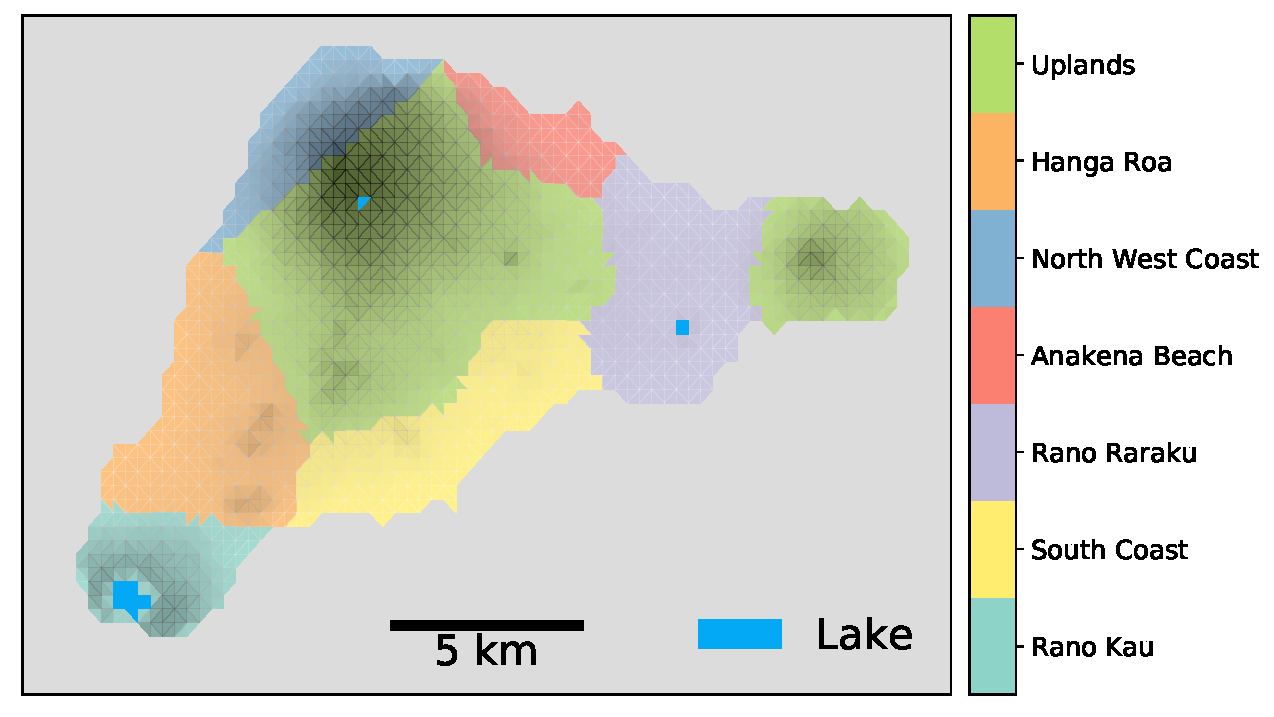
\includegraphics[width=1.0\linewidth]{images/Results/Standard/MapRegionsCoarse}
	\caption{Division of the map into seven separate regions. The black shadow represents elevation.}
	\label{fig:mapregionscoarse}
\end{figure}
Figure \ref{fig:regionalstats} shows the results of the population in each region over time in the ensemble of 15 runs.
Overall, the island shows diverse and heterogeneous population dynamics. 
Some regions, like Hanga Roa and the South Coast (with a little delay), show early extensive growth followed by a steep decline of the population.
The population around Rano Raraku grows nearly linearly and then, as in the Uplands, declines less strongly after the peak.
In some single realisations, this effect is more pronounced than in the ensemble mean.
The small, less arable regions at Rano Kau, the North West Coast, or Anakena Beach, show some population growth following the abandonment of other, more favourable regions.
The population size in these regions then either declines close to linearly or even remains at the same level for nearly $200$ years.
\begin{figure}
	\centering
	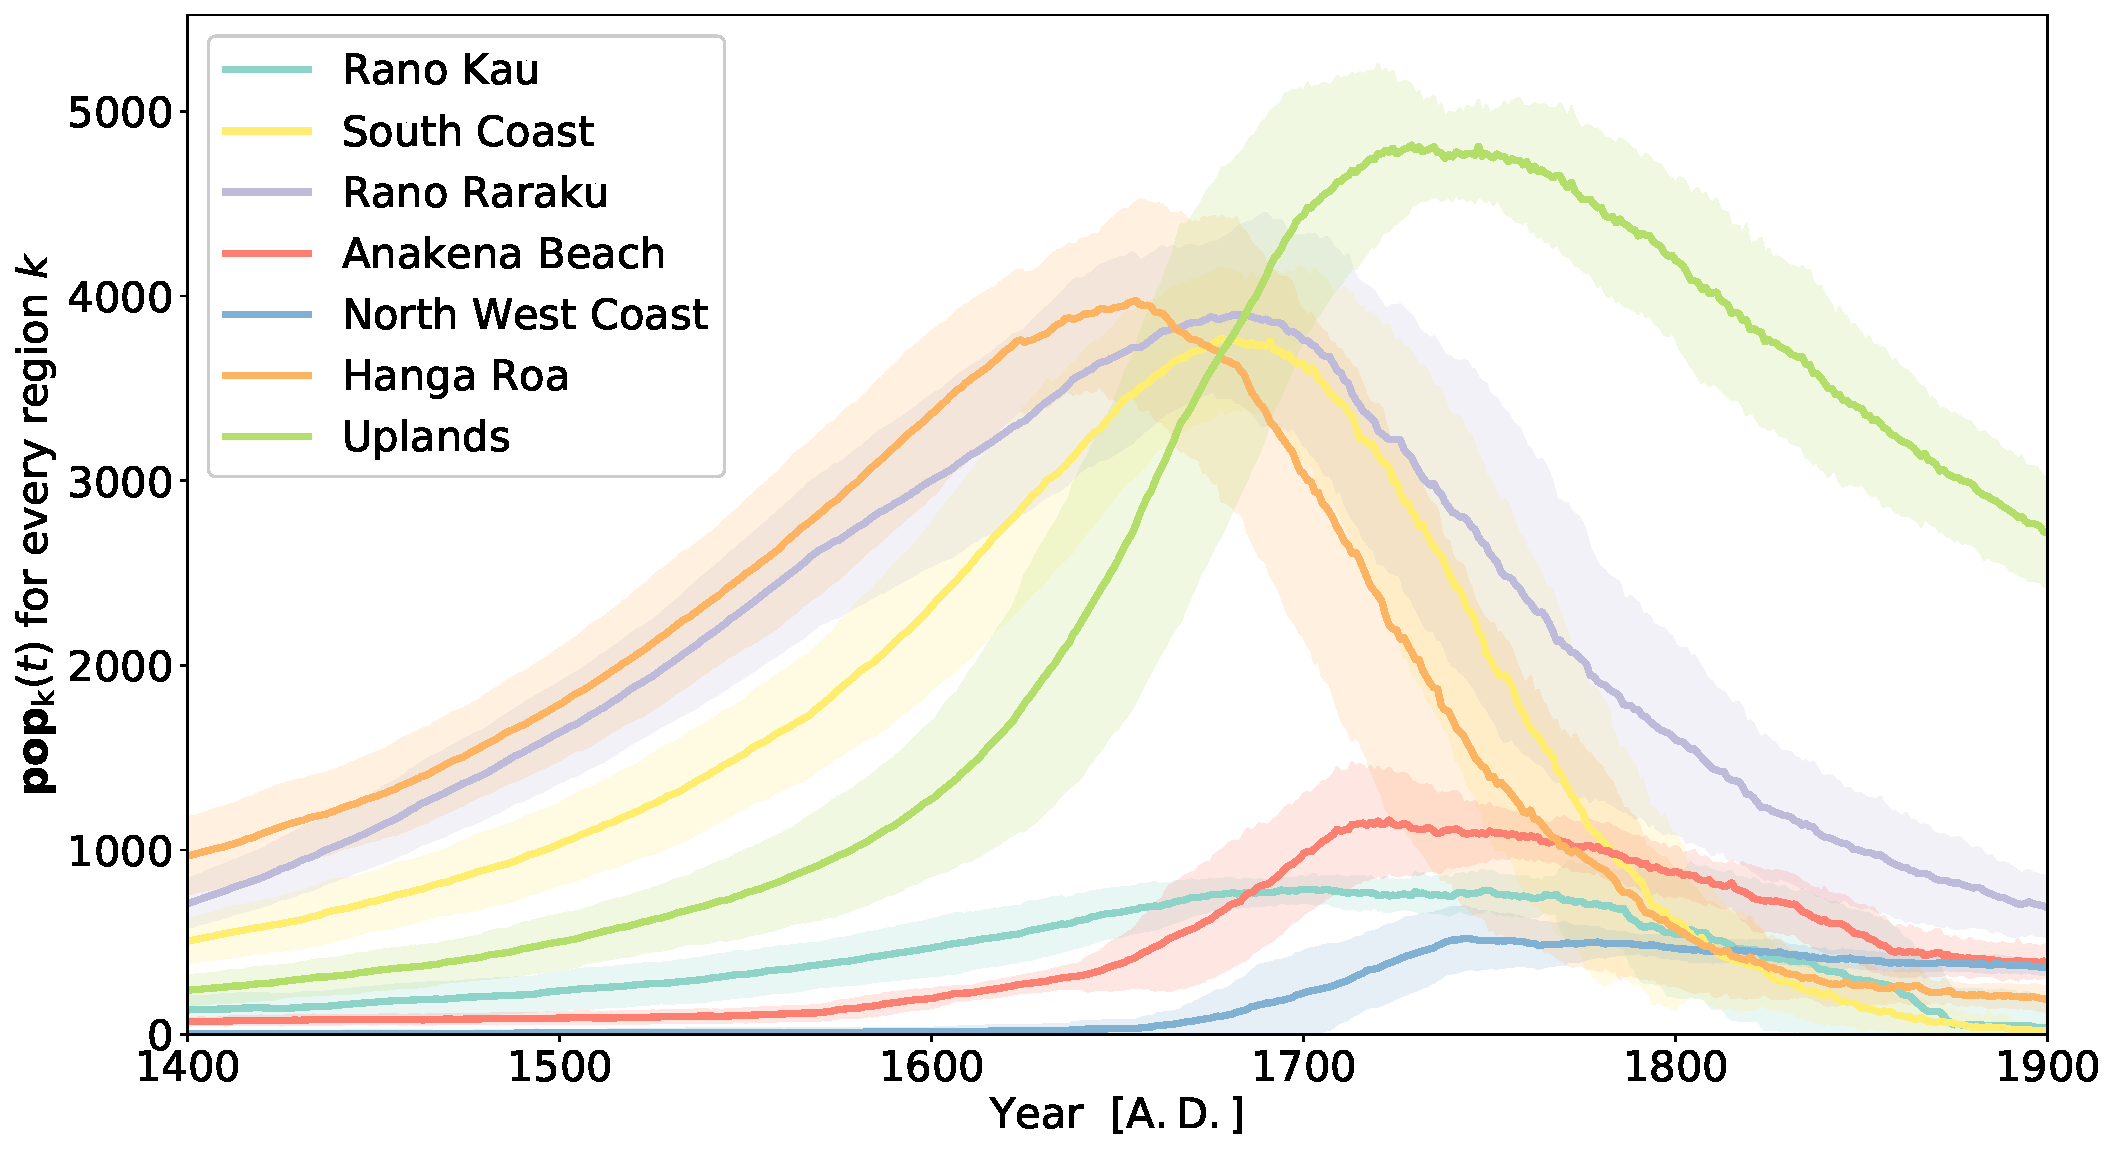
\includegraphics[width=1.0\linewidth]{images/Results/Standard/RegionalStatsEnsembleOnly}
	\caption{The population dynamics of each separate region defined in Figure \ref{fig:mapregionscoarse} as an ensemble of 15 single realisations.}
	\label{fig:regionalstats}
\end{figure}
Given these strong variations between different regions, caution should be exercised when extrapolating results obtained from archaeological evidence in specific regions to the whole island. 
This modelling study, however, gives indications about the implications of these regional differences for the whole island.

\FloatBarrier
\section{Experiments and Sensitivity Analysis}

\subsection{Abundance of and Requirements for Resources}
%\paragraph{Aggregate Dynamics for different choices of parameters mainly influencing the Total Population Dynamics --> Different theories of total population dynamics replicated}
%Statistics Plots for a
%\begin{itemize}
%	\item Run with low N fixation (instead of high)
%	\item Run with tree regeneration and high N fixation
%	\item Run with tree regeneration and low N fixation
%\end{itemize}
%In the making


\paragraph{Outcomes Consistent with Different Narratives.}
The standard run configuration used in the Section \ref{sec:std} reproduces a boom and bust dynamics. 
However, the parameters in this configuration are debatable and this uncertainty lies at the heart of the contrasting views of Easter Island's historical development.
In particular, the (spatially varying) farming yields on Easter Island soils (here expressed via $F_{\rm Req, \ pP}$ and, correspondingly, $F_{\rm PI}(c)$) are uncertain.
Also, $T_\text{Req, pP}$ is speculative and in fact probably highly heterogeneous between agents.
These constant parameters, $F_{\rm Req, \ pP}$ and $T_{\rm Req\ pP}$, determine the amount of tree harvesting and farmland occupation and, thus, are crucial for the temporal development of the island's environment and the peak population size. 
In a series of experiments, I change these constants, $F_{\rm Req, \ pP}$ and $T_{\rm Req\ pP}$, and/or additionally allow tree regeneration.
Figure \ref{fig:ensemblestatisticsalltheories} shows four different scenarios with strongly varying results.
\begin{itemize}
	\item The upper left panel shows the standard run configuration, which considers the high Nitrogen fixation scenario of \citet{Puleston2017} for $F_\text{Req, pP}$ and without tree regeneration.
	\item The upper right panel, shows the case with low Nitrogen fixation by \citet{Puleston2017}, i.e.\ agents have a higher requirement of farmed land per person.
	Population size (blue) peaks earlier and at a smaller number (ca. $6000$ people) and the consequent decrease is slower with a rate close to $-0.2\%/yr$.
	The amount of burnt trees (red) especially in the first phase with constant population growth rate is higher in this scenario, because more arable land needs to be occupied by the agents.
	\item In the corresponding bottom panels, tree regeneration is enabled with parameters set as in Table \ref{tab:sensitivity}. 
	For both cases with tree regrowth (lower panels), a heterogeneous pattern of agents with different tree preferences emerges with some areas characterised by agents with maximum, some with minimum tree preference (not shown here).
	\begin{itemize}
		\item In the lower left panel, with high Nitrogen fixation, a population of nearly $24\cdot10^3$ individuals is reached at a later time than in the standard setting. After that peak, the population size then declines slowly until an equilibrium between tree renewal and tree cutting is reached with all arable sites being occupied after $1700\, {\rm A.D.}$.
		There are two temporarily separated peaks in the amount of burnt trees around $1300\, {\rm A.D.}$ and $1650\, {\rm A.D.}$.
		\item In the lower right panel, with low Nitrogen fixation, population peaks at a similar level and time compared to the case without tree regrowth.
		Here, however, the population size remains constant roughly at this peak level with all arable sites being occupied before $1600\, {\rm A.D.}$.
	\end{itemize}
	%However, the peak population size occurs later and at respectively higher levels if the resource trees replenishes and the resource 
	%After reaching the peak, the population size decreases slowly and levels off at an equilibrium value for both scenarios, in which the renewal of trees matches the requirement of the population and the amount of farming land required remains constant.
	%In both cases with tree regrowth, all available arable sites are farmed in $1600\, {\rm A.D.}$ and $1700\, {\rm A.D.}$ (and mostly remain occupied throughout the rest of the simulation).	

\end{itemize}
A further experiment (not shown) with increased tree requirement per person $T_\text{Req, pP}(t)=10\,{\rm \frac{Trees}{yr\cdot person}}$ yields a similar boom and bust as in the standard run configuration but the population size peaks earlier and, thus, at a lower peak level ($\sim 13000$), and with more intense deforestation.
 
The population dynamics obtained from these different scenarios varying only in two or three parameters reflect the contrasting storylines about the historic population dynamics of Easter Island currently present in the scientific debate.
In particular, the low Nitrogen fixation scenario\footnote{consistent with \citet{Hunt2007}'s assumption of low quality soil} resulting in constant or only slowly decreasing population size decline corresponds to the genocidal \citep{Hunt2007} or slow-demise \citep{Brandt2015} views.
%The standard run (and run with lower $T_{\rm Req, \ pP}$) corresponds more to the ecocidal view as described before.

% correspond to some degree to the different narratives.

%If tree regrowth is enabled over time all arable cells are turned into farming sites and trees are obtained from non-viable sites.
%An heterogeneous pattern of agents with different tree preferences emerges with some areas dominated by agents at maximum, some at minimum tree preference.
% pattern of areas with high tree densities and high farming densities is obtained. 
%\TODO!!

\begin{figure}
	\centering
	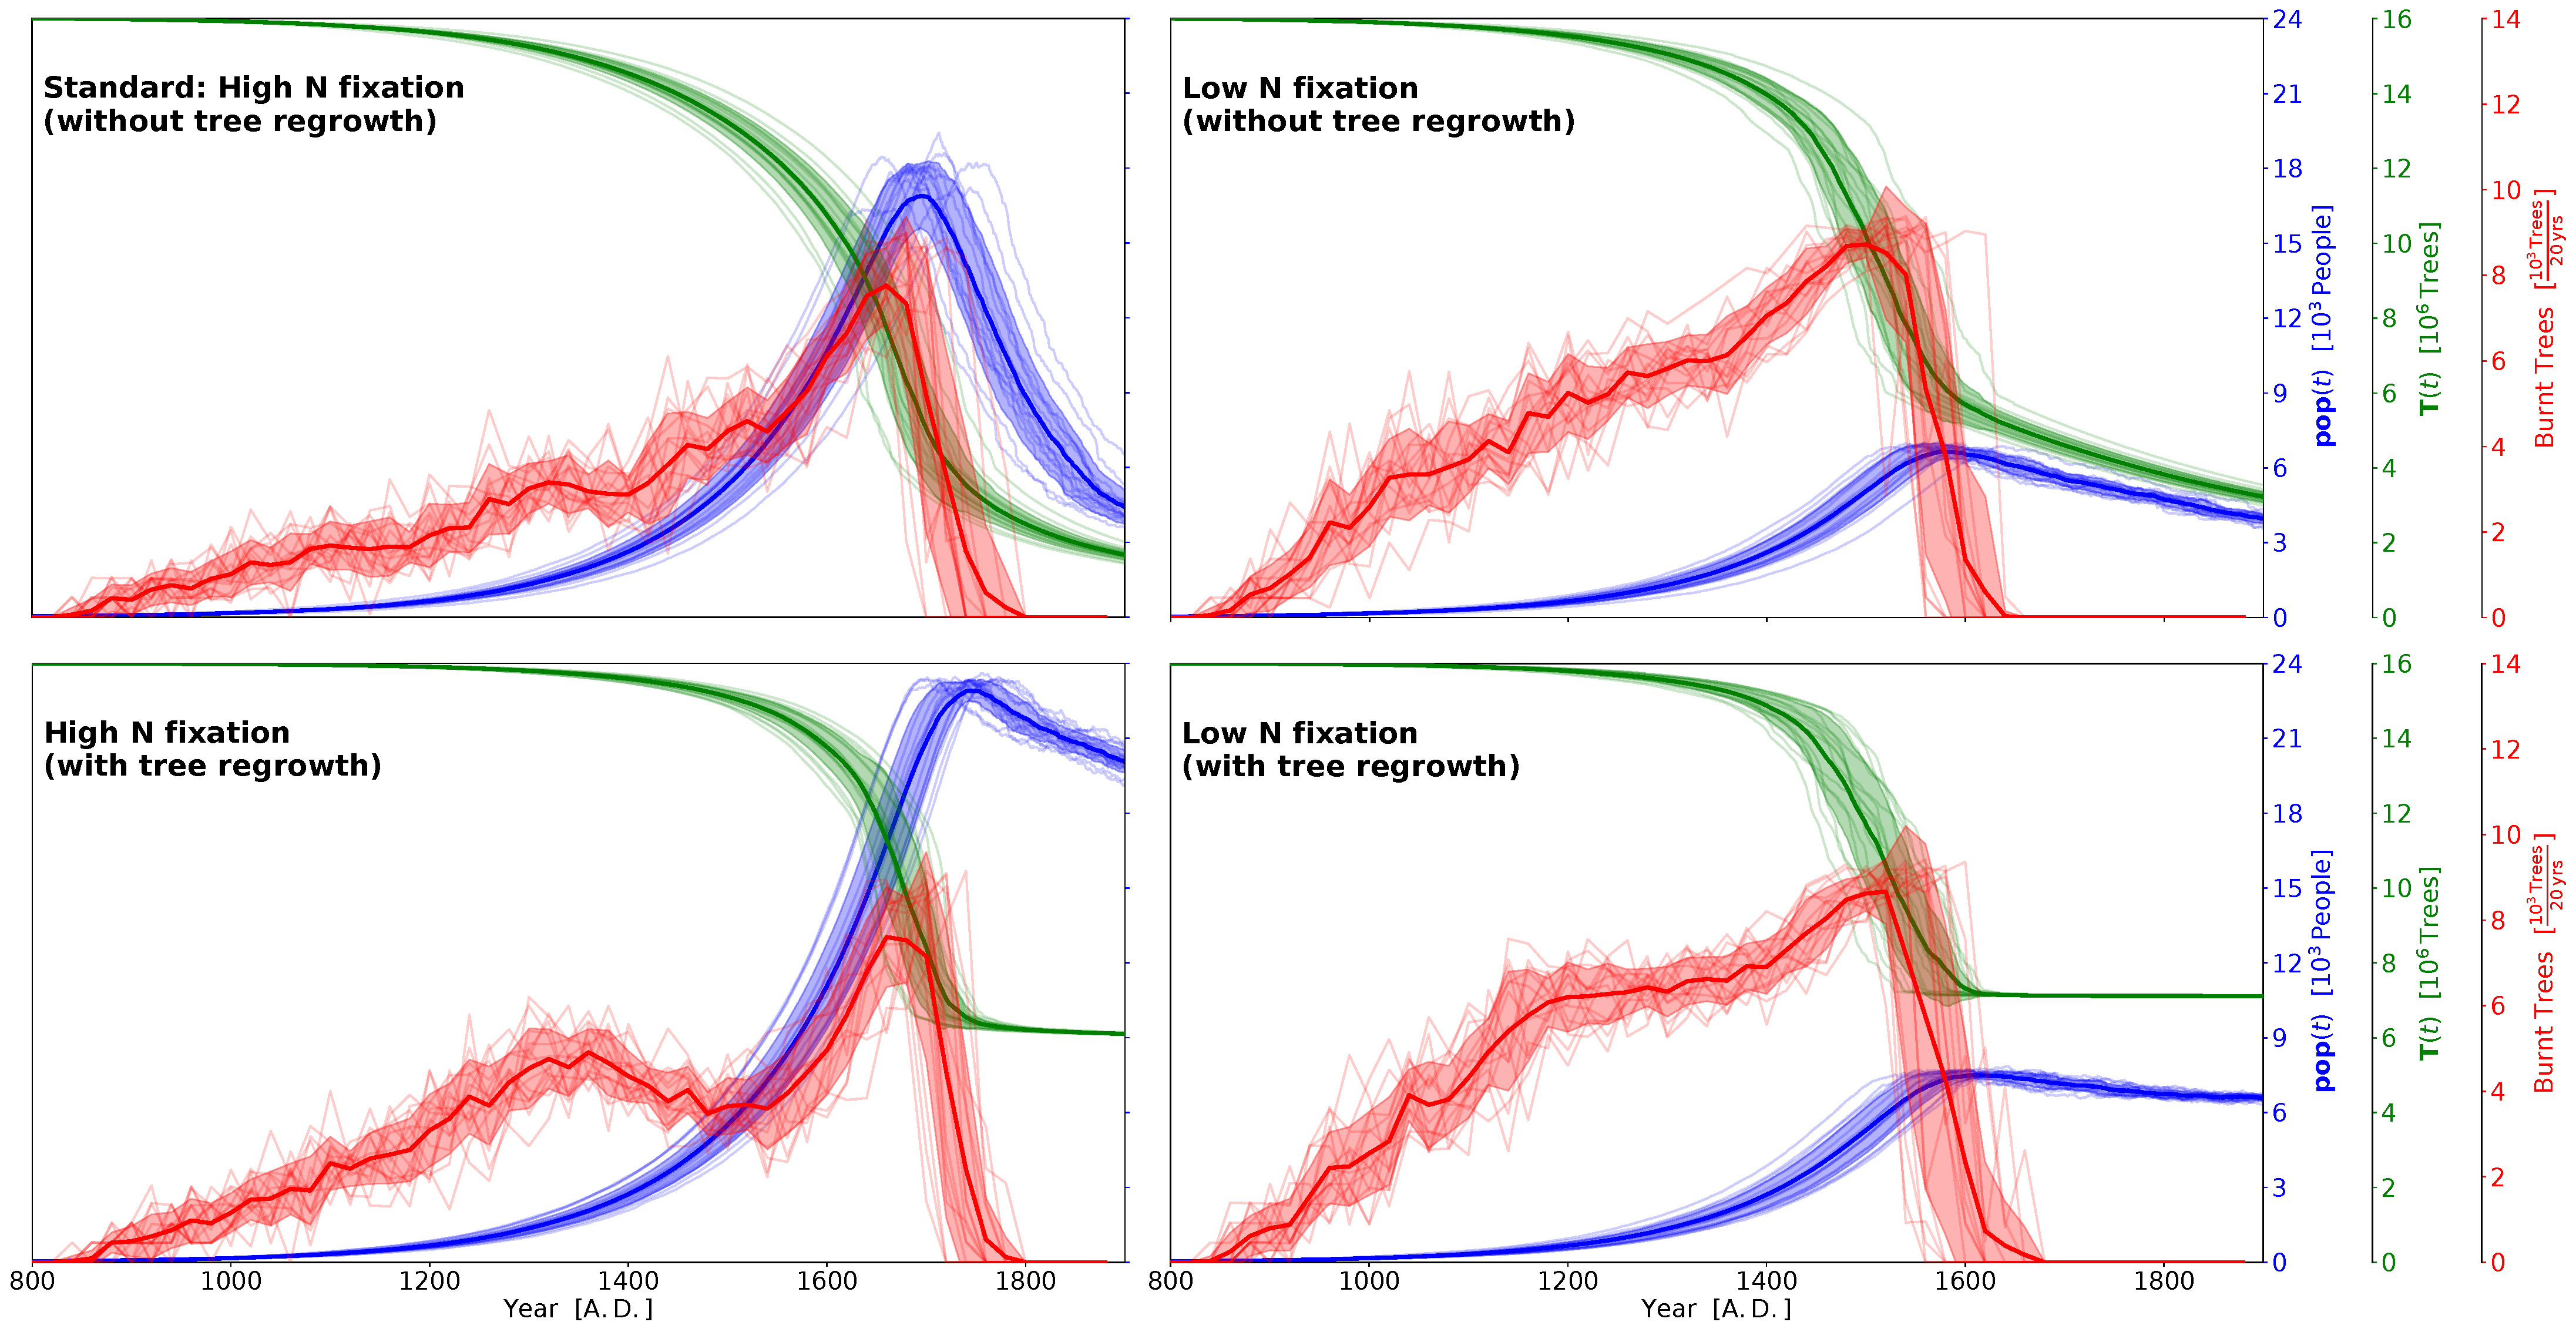
\includegraphics[width=1.3\textwidth, center]{images/Results/Standard/EnsembleStatistics_allTheories}
	\caption{Dynamics of aggregate population size, trees, and burnt trees for four different parameter settings: The high or low N fixation scenario determining the amount of arable land required per person in combination with disabled/enabled tree regrowth.
		All panels show mean dynamics obtained from an ensemble of 15 runs.}
	\label{fig:ensemblestatisticsalltheories}
\end{figure}

\subsection{Resource Search Radii}
\begin{figure}
	\centering
	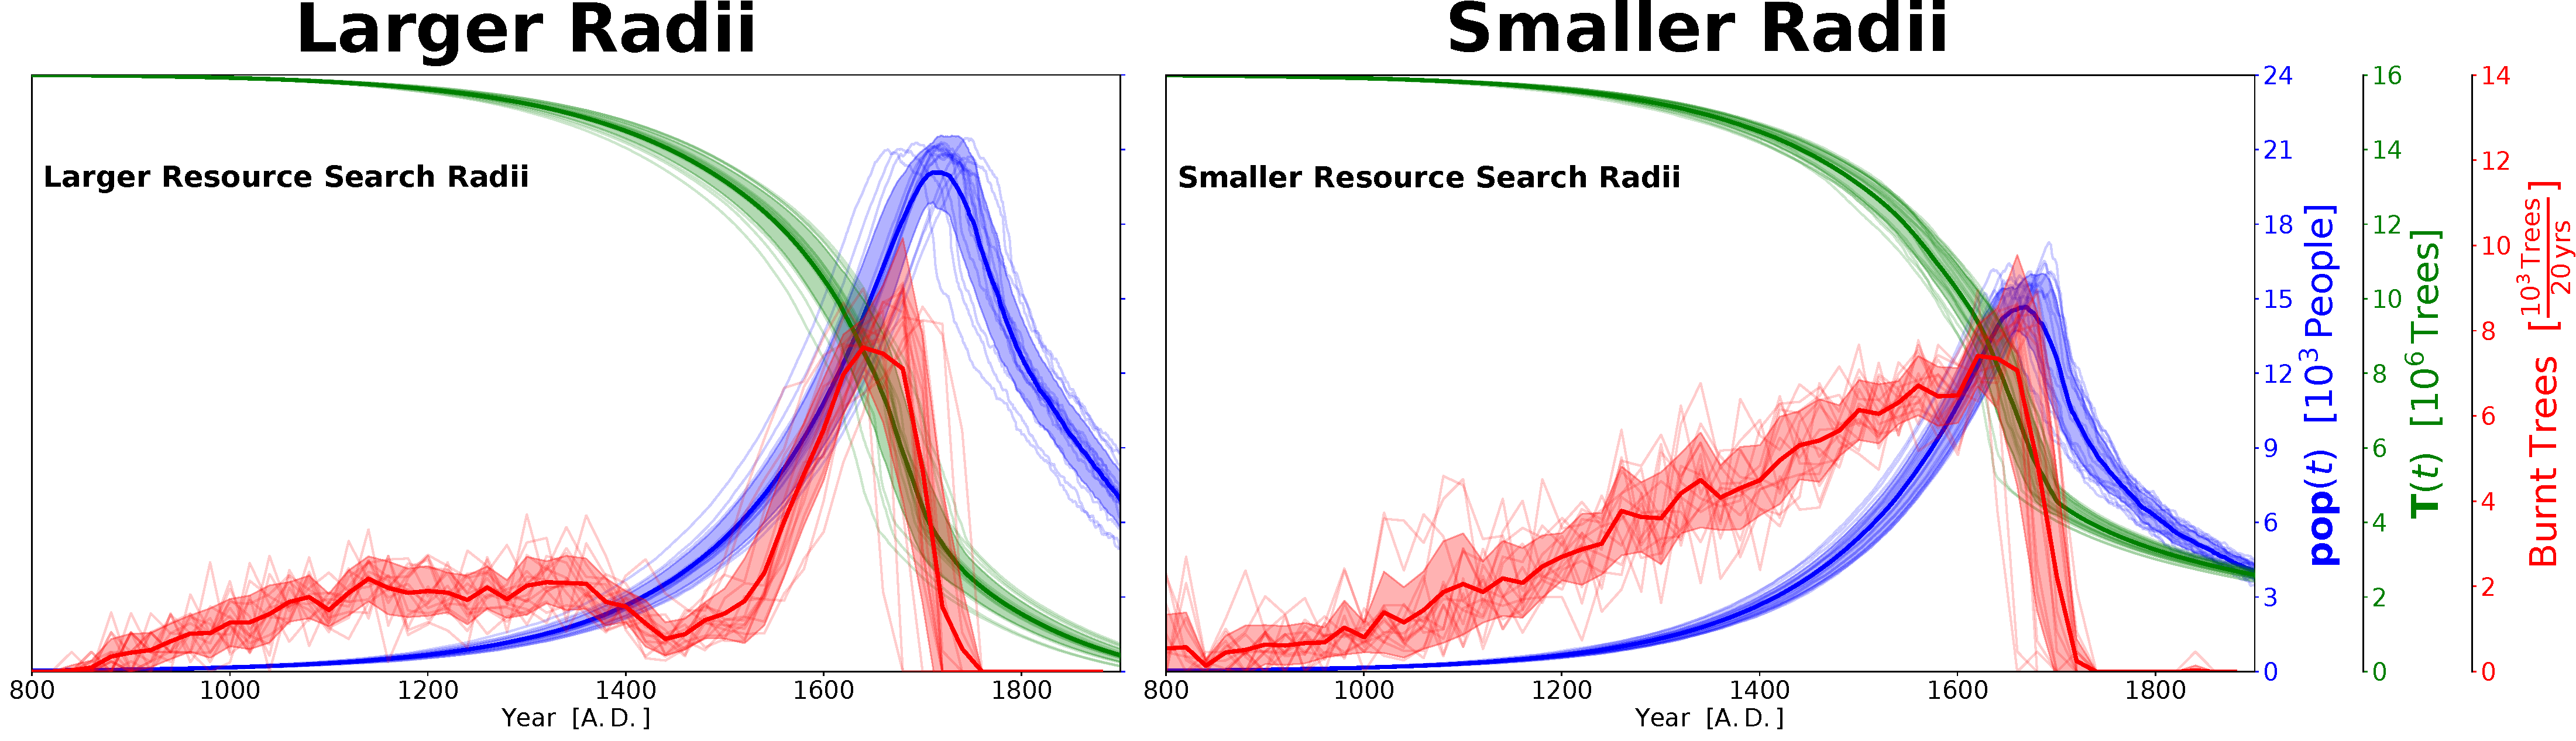
\includegraphics[width=1.3\linewidth, center]{images/Results/EnsembleStatistics_largersmallerRad}
	\caption{Dynamics of aggregate variables (as before) for variation of the resource search radii: The left panel shows runs with factor $2$ larger radii: $r_{\rm T}=4\, {\rm km}$ and $r_{\rm F}=2\, {\rm km}$; The right panel with factor $1/2$ smaller radii: $r_{\rm T}=1\, {\rm km}$ and $r_{\rm F}=0.5\, {\rm km}$. While changing the resource search radii does not change resource requirements or abundance, all aggregate variables depend strongly on this choice.}
	\label{fig:ensemblestatisticslargersmallerrad}
\end{figure}

\paragraph{Aggregate Dynamics.}
In Figure \ref{fig:ensemblestatisticslargersmallerrad}, I present a sensitivity analysis of the resource search radii, which are increased or decreased by a factor of $2$ (left) or  $1/2$ (right), respectively, compared to the standard run configuration. 
For larger radius the peak population size increases, deforestation intensifies and the amount of burnt trees remains low for a long time but rises steeply around $1600\, {\rm A.D.}$.
At smaller radius, the peak population size strongly decreases, deforestation is less intense, and burning of trees increases linearly until a cut-off.
Variation of the resource search radius has a non-trivial influence on the aggregate dynamics.
While a larger (or smaller) radius increases (or decreases) an agent's access to resources at its current location, it does not change the amount of available resources on the island or required resources by the agents.
As Figure \ref{fig:ensemblestatisticslargersmallerrad} shows, the differences of the results between those scenarios are significant. 
Even though the carrying capacity of the island with respect to the amount of resources is the same, the agent's harvest behaviour is restricted by its local context and, hence, this lack of either available arable land or trees in the local environment changes the shape of the aggregate dynamics.

\paragraph{Social Structure}
It is clear that the social and economic structure of the Easter Island population is much more complex than the independent, small households of a few dozen people acting independently and myopically as assumed in this model. 
E.g.\ \citet{Diamond2011} describes the existence of roughly a dozen clans or chiefdoms. \citet{Puleston2017} consider an economic structure formed by elite and working classes.
Also, there is clear evidence of exchange of goods between households and clans or chiefdoms, e.g.\ fish, stone tools or the Moai.
Such social structures would also allow for imposing taboos on the harvest of natural resources and increase the sustainability, although with limited effectiveness according to some researchers \citep{Good2006}. 
All of these complex, institutional structures based on agent-agent interactions are not considered here, but each agent farms and deforests individually.
Including such social and political institutions would smooth the impacts of changing the resource search radii (or the local confinement of agents) and, thus, might lead to different population dynamics.

\paragraph{Outlook: Clusters and Chiefdoms.}
The model presented here can be extended to show the emergence of clustered agents that cooperatively harvest resources.
E.g.\ Figure \ref{fig:clusterstds1650} shows the centre points of $7$ clusters obtained by k-Means clustering of the three dimensional space spanned by the agent's position and tree preference trait, $\left( x_{\rm i}, y_{\rm i}, T_\text{Pref, i} \right)(t)$ for agent $i$, in one specific year, $1650\, {\rm A.D.}$ using the python packages \textit{scikit-learn}\footnote{\citet{scikit-learn}} and \textit{yellowbrick}\footnote{\citet{yellowbrick}}.
For all tested years (between $1200$ and $1900\, {\rm A.D.}$) a number of $7$ to $9$ clusters are optimal according to the elbow method\footnote{The elbow is a heuristic to estimate the number of clusters:
	Running the k-Means algorithm with more clusters only linearly decreases the distortion, i.e.\ the sum of the squared distances of an agents 3D state to the cluster centres.}.
While this analysis is very preliminary, clustering might open up the possibility of including stronger links within clusters of agents that tend to move towards each other (e.g.\ negative population density penalty), harvest cooperatively, and increase the resource search radius with the cluster size.
One could even think of including a trading module between clusters (as in \citen{Heckbert2013}).
Future research with this model could investigate more complex economic and social structures and, thereby, overcome one of the major weakness, the self-centred, non-cooperative harvest behaviour of the agents considered here.

\FloatBarrier
\subsection{Population Growth}
\paragraph{Aggregate Dynamics.}
I test the stability of the model results to a less resilient demography.
By increasing the shape parameter of $g(H_{\rm i})(t)$ an agent's population size exhibits a steeper and earlier decline as $H_{\rm i}(t)$ decreases.
%and, thereby, increasing the required happiness to remain at a constant population size, $H_{\rm euq}$ a population decline sets in earlier and more extreme in most cases.
However, in the standard run configuration, happiness of the agents decreases rapidly from $1$ to $0$ typically close to the peak population size and an agent can not find a place sufficient for meeting both resource requirements.
Hence, the results are nearly independent from this variation of the population growth model\footnote{In this simulation the ensemble net population decrease sets in only $10$ years prior to the standard case and at the same peak level.}.
However, for the scenario with tree regrowth 
the stable equilibrium between tree regrowth and tree cutting can sustain fewer individuals (roughly $2000$ less, not shown) for this less resilient population scenario and its higher equilibrium happiness, $H_{\rm equ}$.
%decreases the population size in the stable equilibrium (and the peak) by roughly $2000$ individuals (not shown).

\paragraph{Oversimplified Population Growth.}
The population dynamics in this ABM is subject to several limitations.
The use of the food-limited demography model from \citet{Puleston2017} is strongly simplified here.
E.g.\ I use a different notion of \citet{Puleston2017}'s food ratio, which I express via the effective happiness $H_\text{i}(t)$ reflecting the (smoothed) success in cutting trees and farming.
Also the distinction between survival and fertility rate especially given their age-dependency is entirely neglected.
One major problem with the assumed population dynamics in this model is the fast decrease of effective happiness when the resource, trees, becomes scarce and the agent can not find a place on the island suitable to sustain it with both trees and farming products simultaneously and, therefore, perishes quickly.
Another issue is the unabated exponential growth of the population independent of population density.
The model would greatly benefit from a smarter, more dynamic integration of the demography model by \citet{Puleston2017} and, in general, a more elaborate relation between the tree cutting, farming and population growth.


\subsection{Tree Preference}
%\paragraph{Differences in Burnt Trees, Population Size and Deforestation given the different adaption speed of the tree preference to local environmental changes}
%\begin{itemize}
%	\item Runs with $f_{\rm Tree \ Pref}$ delayed, careful, logistic.
%\end{itemize}

%\paragraph{Impacts on the Aggregate Dynamics of Different Adaption Strategies}
The change of the tree preference in response to local deforestation is the only far-sighted adaptation mechanism of the agents in the harvest process in response to environmental degradation.
In the standard run configuration, an agent's tree preference responds linearly to the removal of trees.
In Section \ref{sec:agentprops}, I presented three alternative adaptation strategies: Delayed, faster (i.e.\ with foresight), and logistic adaptation (first delayed, then faster) (see Figure \ref{fig:TPref_T}).
\begin{figure}
	\centering
	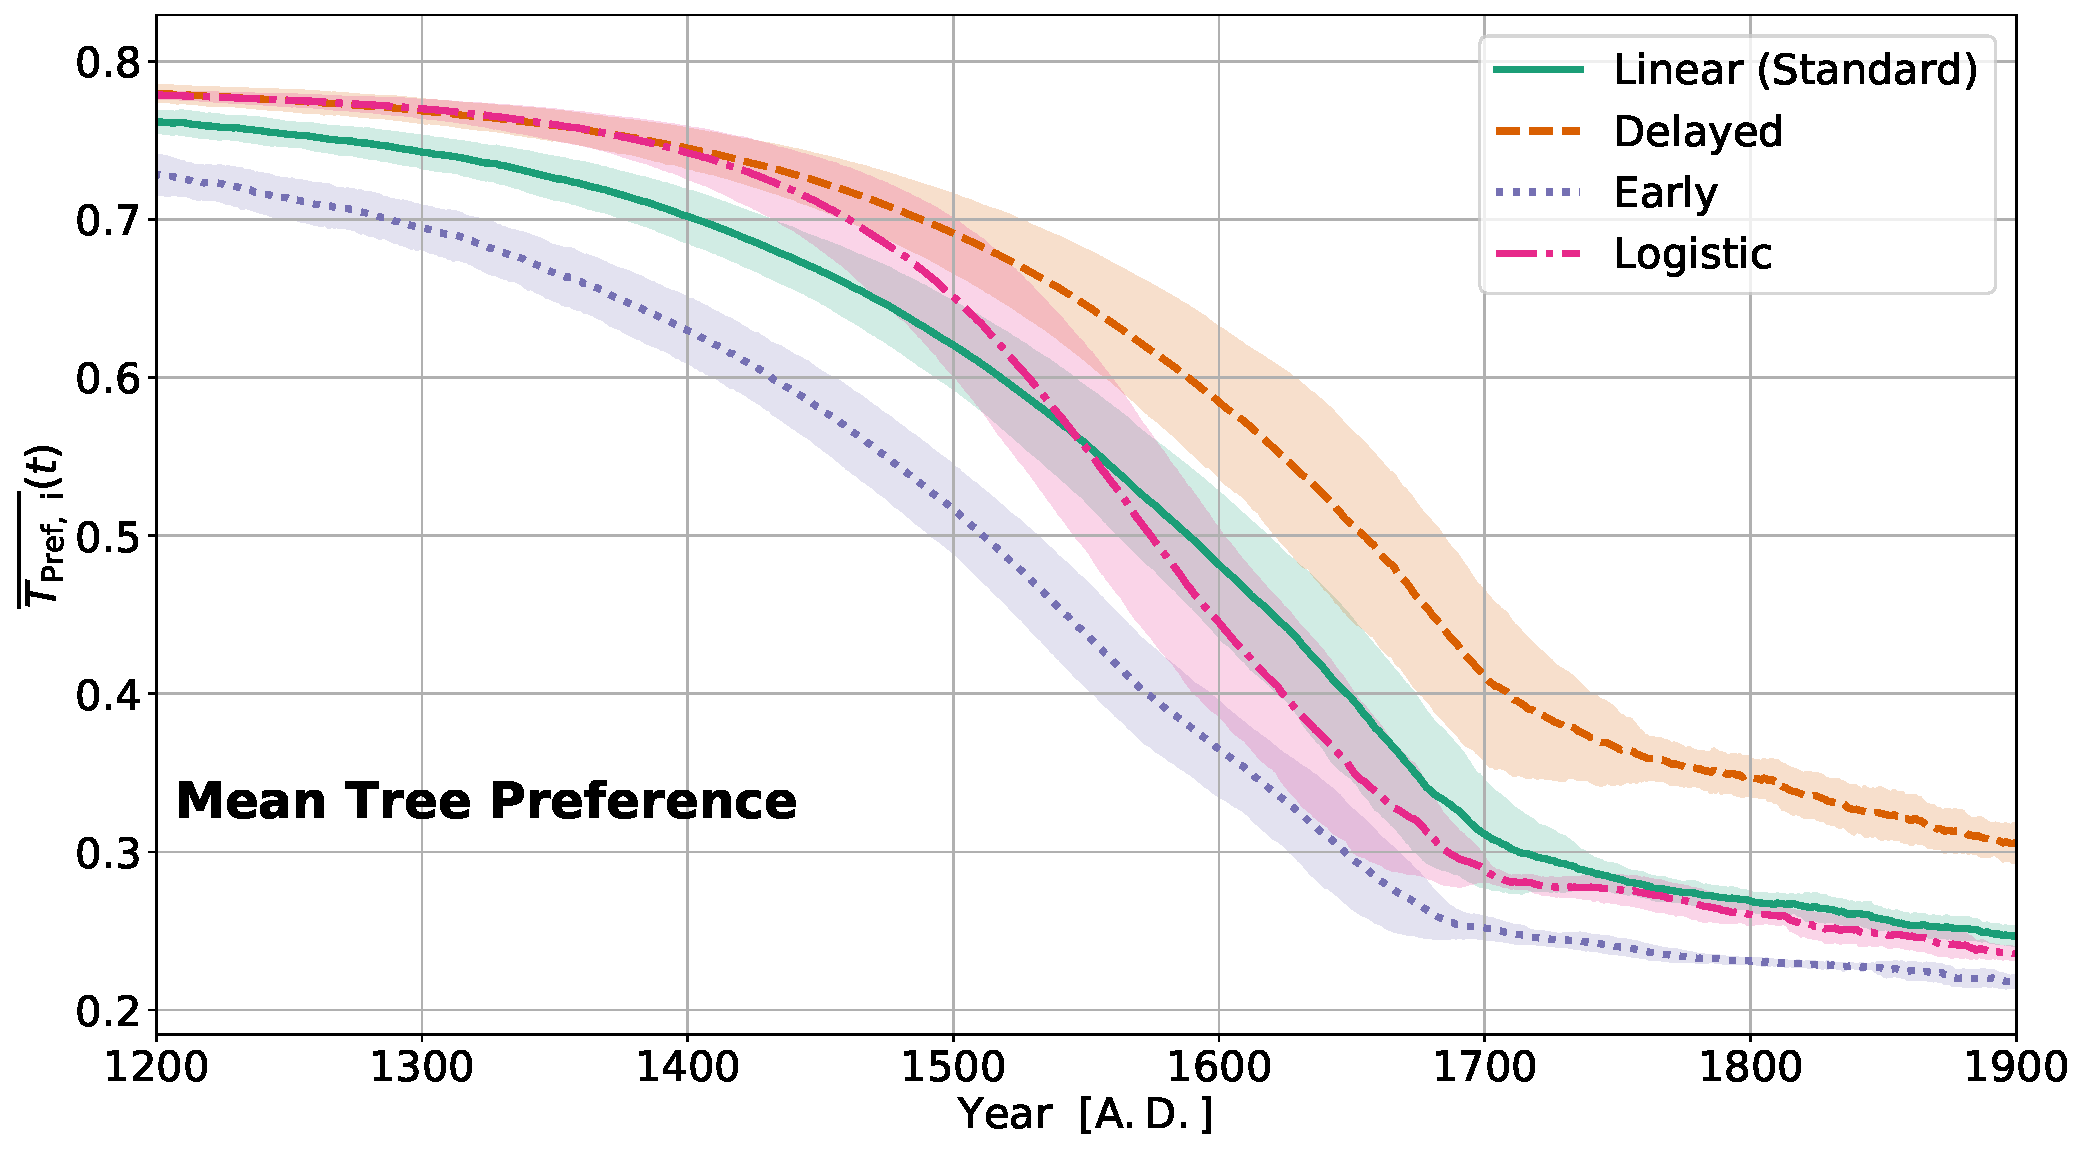
\includegraphics[width=1\linewidth]{images/Results/TPref/TPrefAdaption_TPref}
	\caption{Mean tree preferences of all agents $\overline{T_\text{Pref, i}(t)}$ over time from an ensemble of each 15 different model realisations with different strategies to adapt the tree preference to the changing local tree density: Linear (standard setting), delayed, faster, or logistic (all shown in Figure \ref{fig:TPref_T}).}
	\label{fig:tprefadaptiontpref}
\end{figure}
The mean tree preference of all agents, $\overline{T_\text{Pref, i}(t)}$, is shown in Figure \ref{fig:tprefadaptiontpref} for ensembles of 15 realisations.
The corresponding population dynamics is shown in Figure \ref{fig:tprefadaptionpopulationsize}.
The population size in the fast adaptation scenario peaks at a high value (and later) than in the other cases.
The logistic formulation produces population dynamics that first resemble the case with delayed adaptation and later converges to the case with (standard) linear adaptation. 
By $1900\, {\rm A.D.}$, the population size is nearly twice as high for a fast vs.\ a delayed adapting society.
Similarly, the dynamics of deforestation (Figure \ref{fig:tprefadaptiontrees}) and of burnt trees (Figure \ref{fig:tprefadaptionburnttrees}) depend on the tree preference adaptation strategy. 
E.g.\ while in the case with fast adaptation of the tree preference, the amount of burnt trees increases continuously from beginning to peak, especially in the case with delayed and logistic adaptation, it remains constant (or even decreases) between $1300$ and $1500\,{\rm A.D.}$ followed by a sharp increase afterwards.
The summed amount of burnt trees is largest in the case with fast adaptation ($5.3\cdot 10^6$), compared to cases with linear ($4.3\cdot 10^6$), logistic ($4.4\cdot 10^6$) and delayed ($3.3\cdot 10^6$) adaptation.
Counter-intuitively, more trees remain at the end of the simulations in the case with fast adaptation.
The mean happiness of all agents is also slightly higher (or equivalent) for the fast adaptation strategy throughout the time period (not shown).
In summary, the specific shape of the adaptation of the tree preference to the local environmental change has a non-trivial influence on the aggregate dynamics.

The results show that a fast (and early) adaptation of the tree preference seems to be the best strategy for the agents, maximising the peak and final population size, the amount of trees, and the mean happiness.
While the logistic and linear strategies are quite similar in their aggregate outcomes, the peak population size is smaller for the logistic strategy.
Hence, it seems that a better strategy for a civilisation in this model is to adapt linearly already during the early phase of local tree density change rather than to adapt only slowly and compensating this with a faster pace in the later phase (as in the logistic case).
\begin{figure}
	\centering
	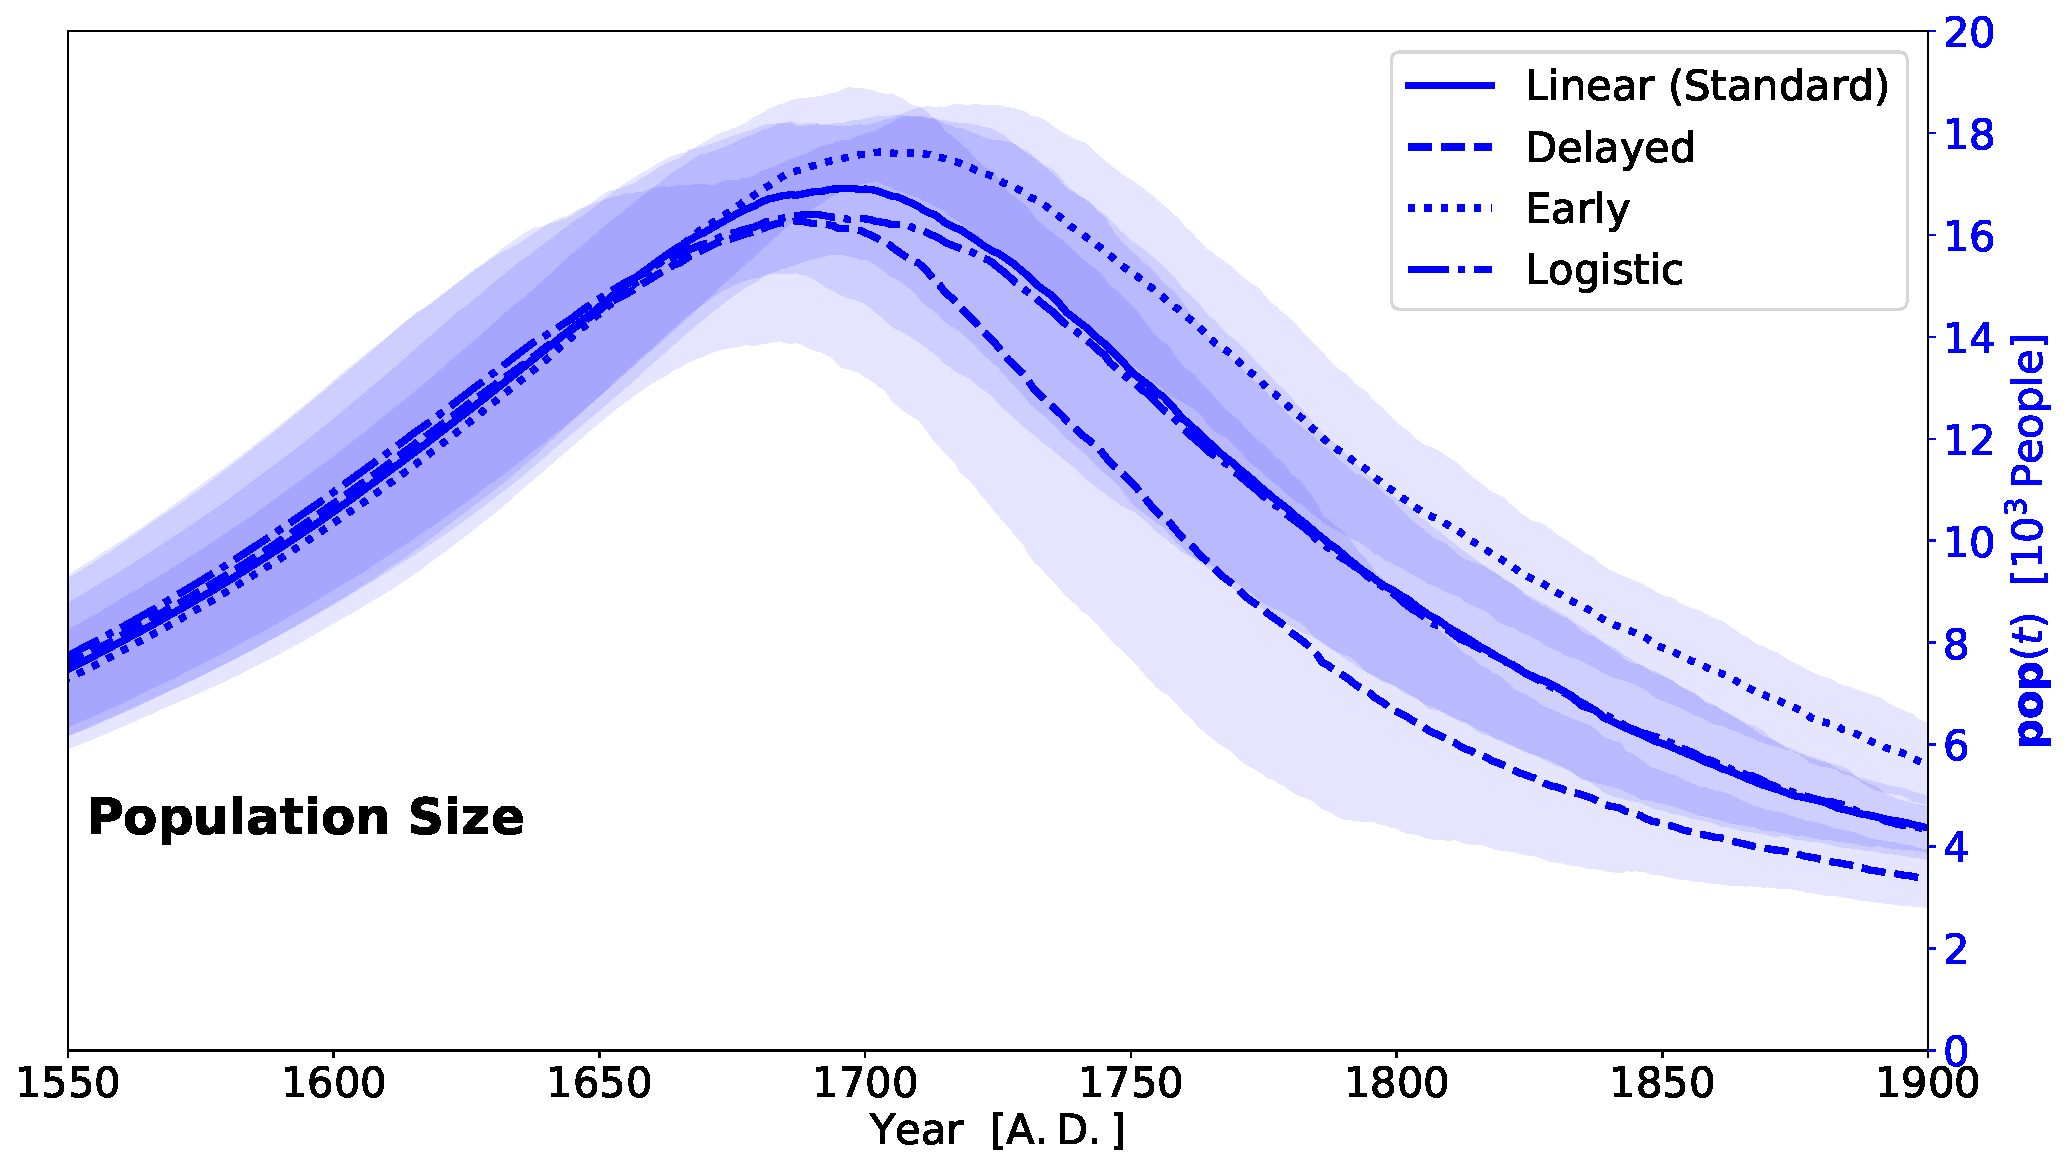
\includegraphics[width=1\linewidth]{images/Results/TPref/TPrefAdaption_Population_Size}
	\caption{Total aggregate population dynamics for different adaptation strategies in relation to tree preference.}
	\label{fig:tprefadaptionpopulationsize}
\end{figure}


\subsection{Moving Strategy}
\paragraph{Spatial and Aggregate Dynamics.}
In the analysis so far, I have distinguished between spatial patterns and aggregate temporal dynamics.
However, the results show that the spatial patterns also have an influence on the aggregate variables, population size, number of trees and number of burnt trees.
Here, I investigate how three different decision making strategies in moving (see also Table \ref{tab:sensitivity}) compare with the standard run. The strategies consider
\begin{itemize}
	\item all penalties equally high, including some stochasticity (the standard run, as described in Figure \ref{fig:STDrull}) 
	\item `only resource' penalties (Figure \ref{fig:resource}), i.e. $\alpha_{\rm T}= \alpha_{\rm F} = 0.5$ and all other weights are zero.
	With this strategy, agents spread out to all locations with access to arable, well-suited land irrespective of distance from freshwater, elevation, slope and population density.
	Consequently, the amount of trees burnt is larger in the period from $1200$ to $1600\, {\rm A.D.}$ as there are no dense population centres in which collective tree cutting contributes to the clearing of land. 
	Population peaks at a slightly later time and at a higher level. 
	The following population size decrease after the peak is steeper and less individuals remain in $1900\, {\rm A.D.}$.
	\item only the `optimal location' with the smallest penalty, i.e.\ a fully deterministic moving decision with $\gamma>>1$ and $\vec{\alpha}$ as in the standard run configuration (Figure \ref{fig:optimal}).
	Interestingly, agents cluster around `highly evaluated' spots leading to a patchy spatial pattern. The aggregated population size (including the peak level), number of burnt trees or tree number are mostly unaffected by this, in comparison to the standard run but the variation in peak population size is smaller.
	\item no penalties or evaluation criteria at all, i.e.\ agents ignore all penalties ($\gamma = 0$) and perform a `Trial\&Error Hopping' (Figure \ref{fig:hop}).
	Hence, an agent might `hop' around in consecutive years until a spot with sufficient resource access is found, but burn trees to set up farms in all intermediate locations.
	This process delays the population growth, and, consequently, the population size peaks a century later (shortly before $1800\, {\rm A.D.}$) but at a similar peak size compared to the standard run. The peak is followed by a rapid decline (up to $2\%$ per year) to a third of the population size within less than a century.
\end{itemize}
\begin{figure}
	\centering
	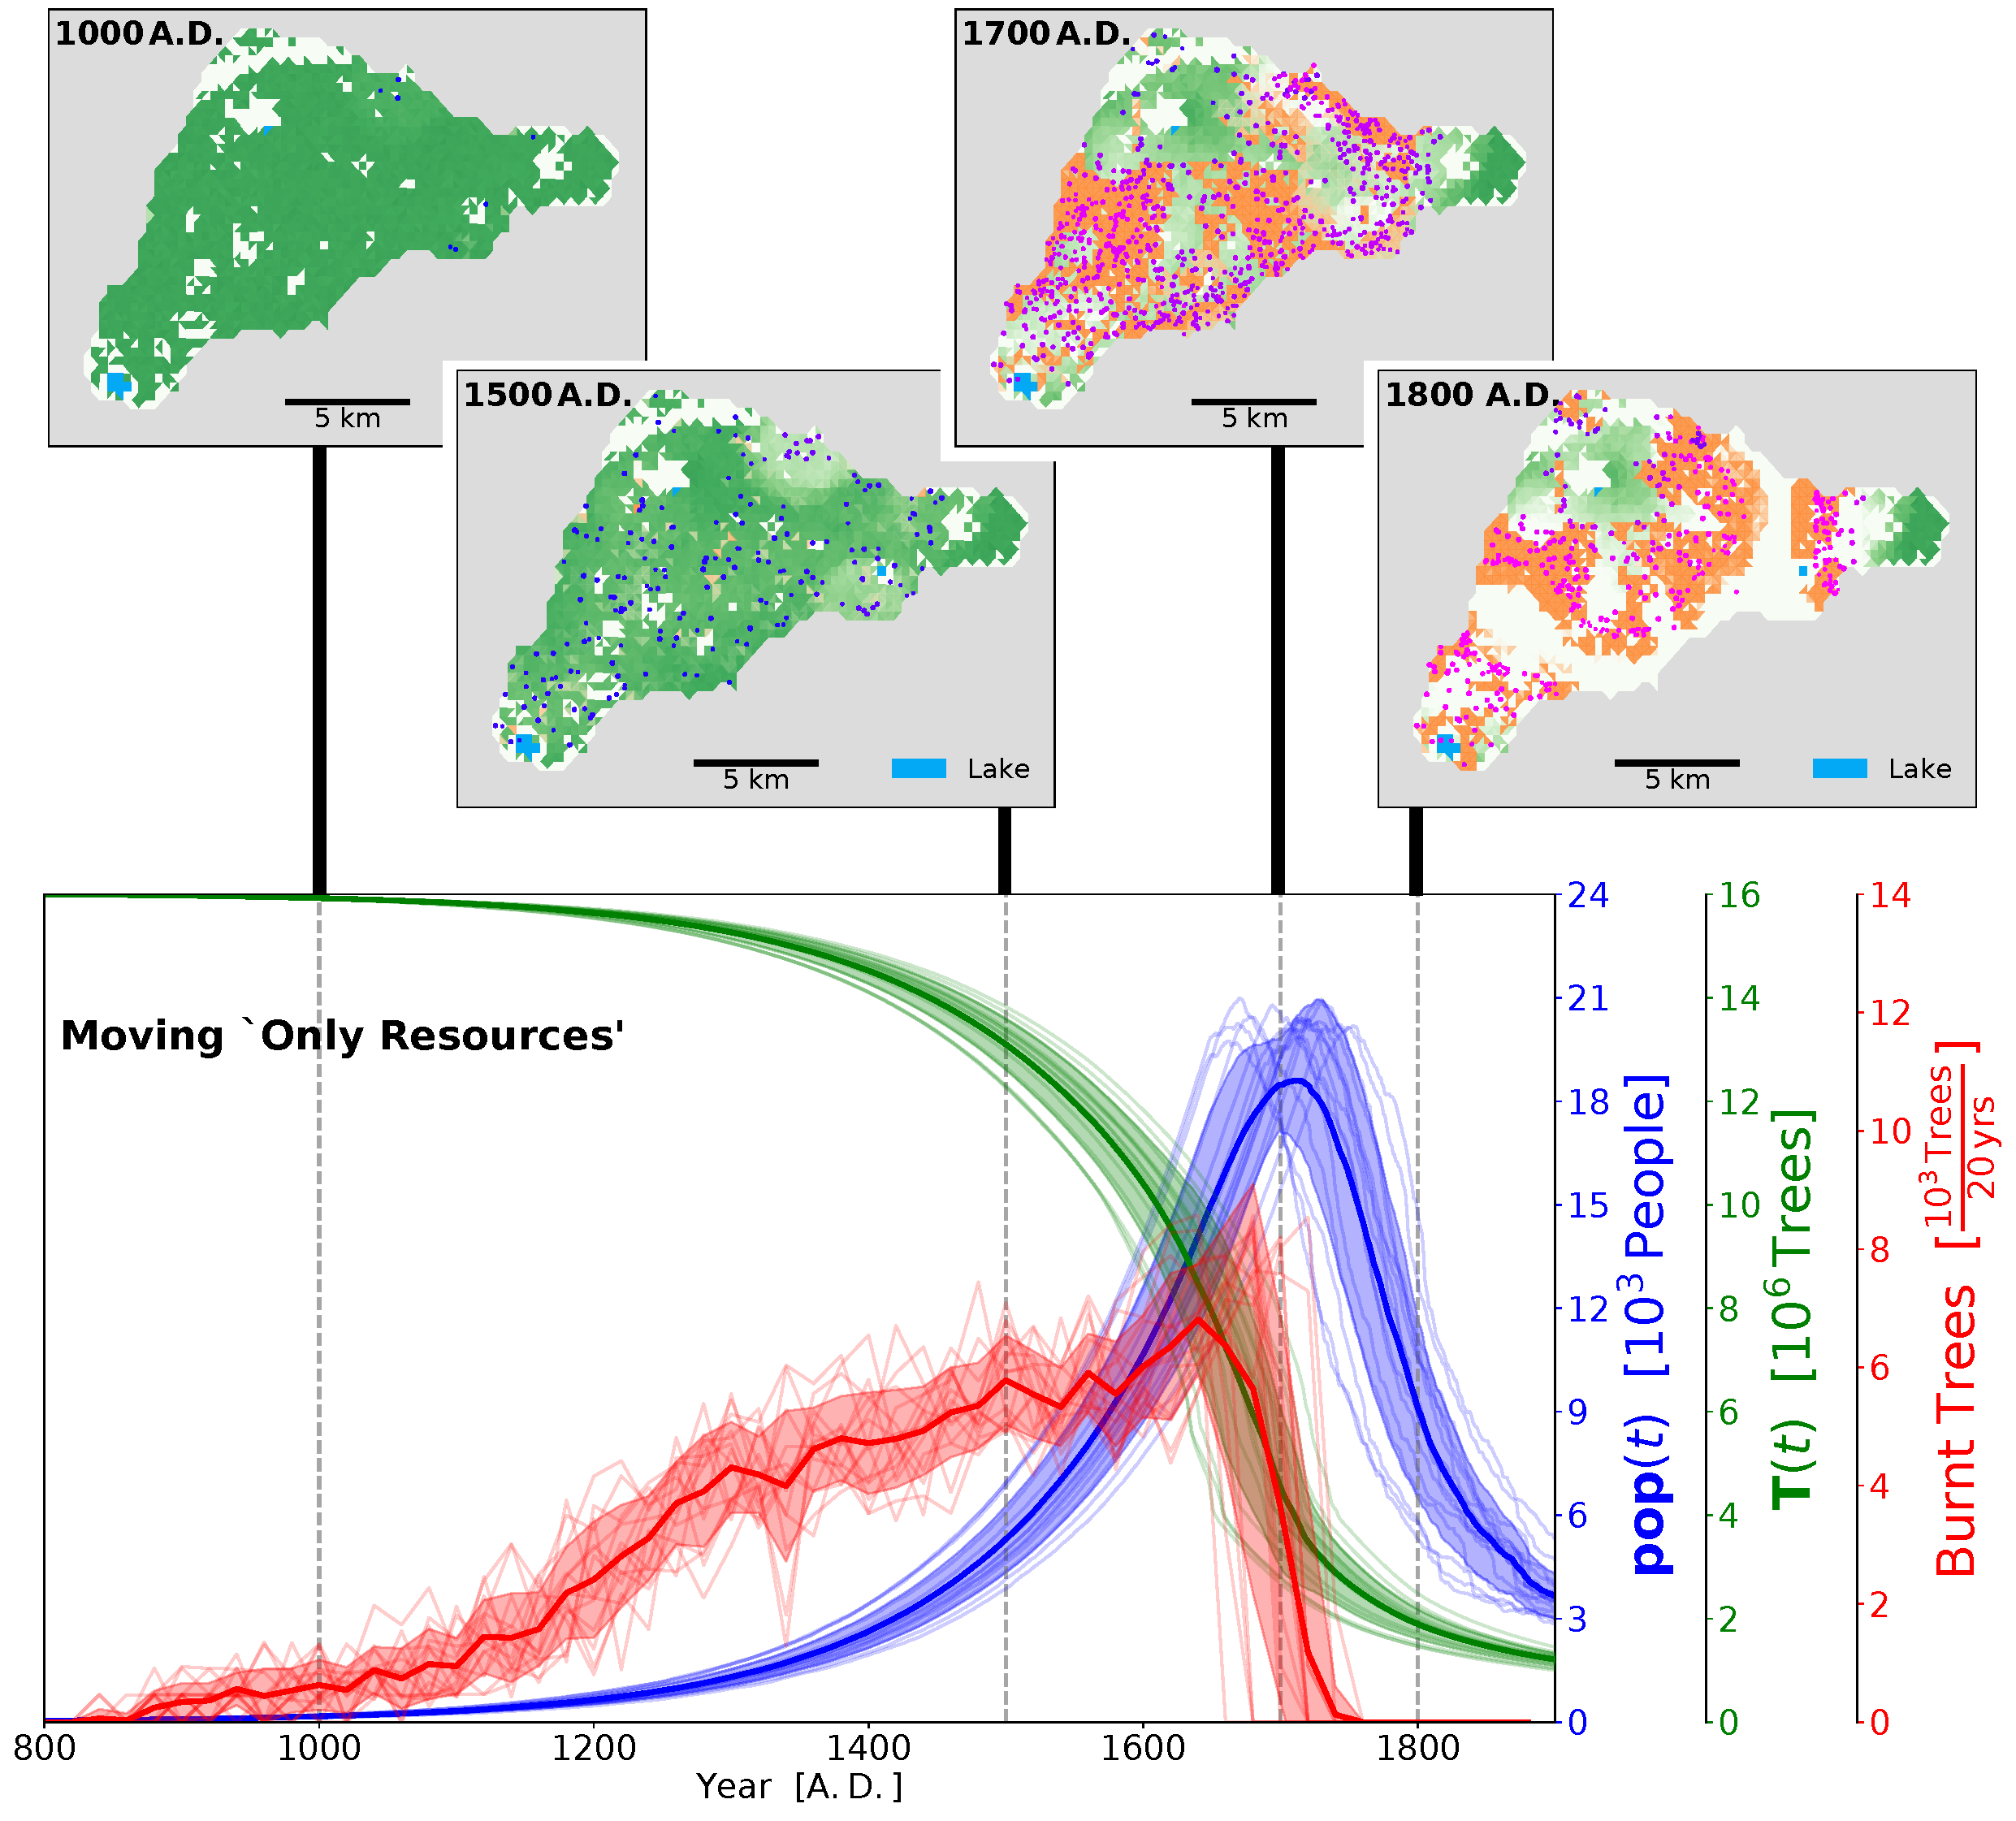
\includegraphics[width=1\textwidth]{images/Results/Moving/alphaResource_EnsembleStatistics+Panels}
	\caption{Moving strategy `Only Resources'.}
	\label{fig:resource}
\end{figure}
\begin{figure}
	\centering
	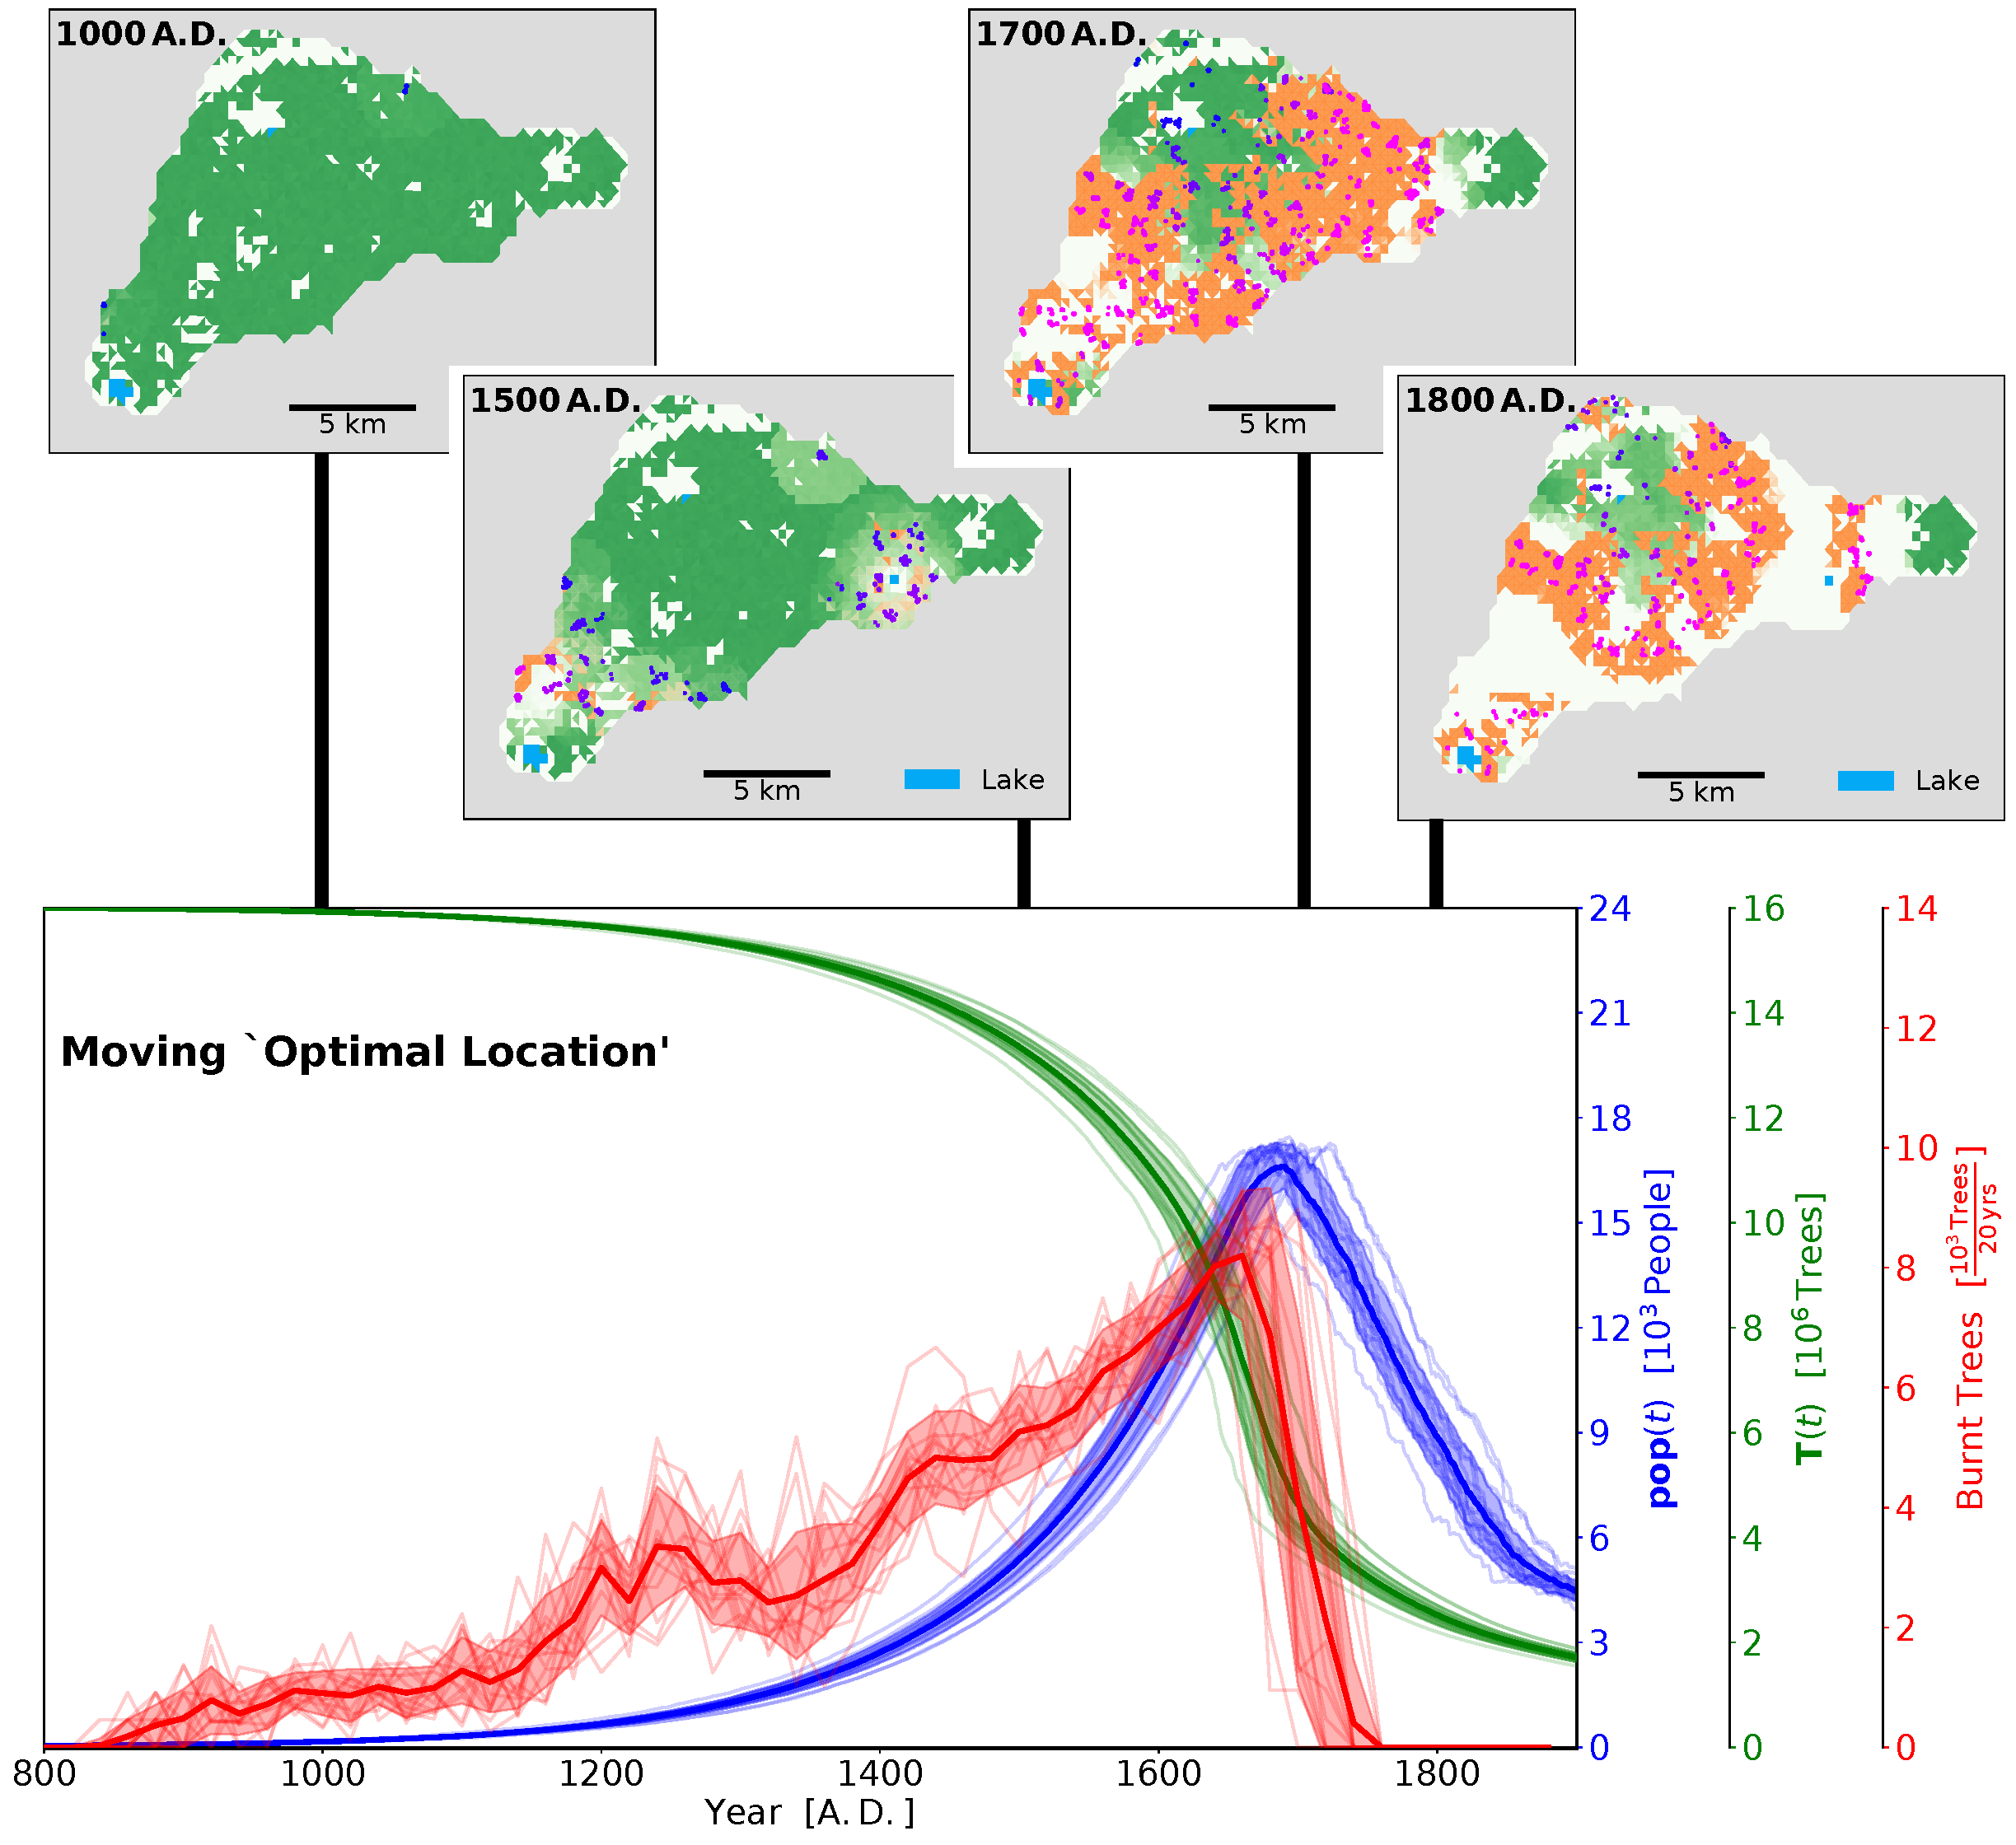
\includegraphics[width=1\textwidth]{images/Results/Moving/alphaDeterministic_EnsembleStatistics+Panels}
	\caption{Moving strategy `Optimal Location'.}
	\label{fig:optimal}
\end{figure}
\begin{figure}
	\centering
	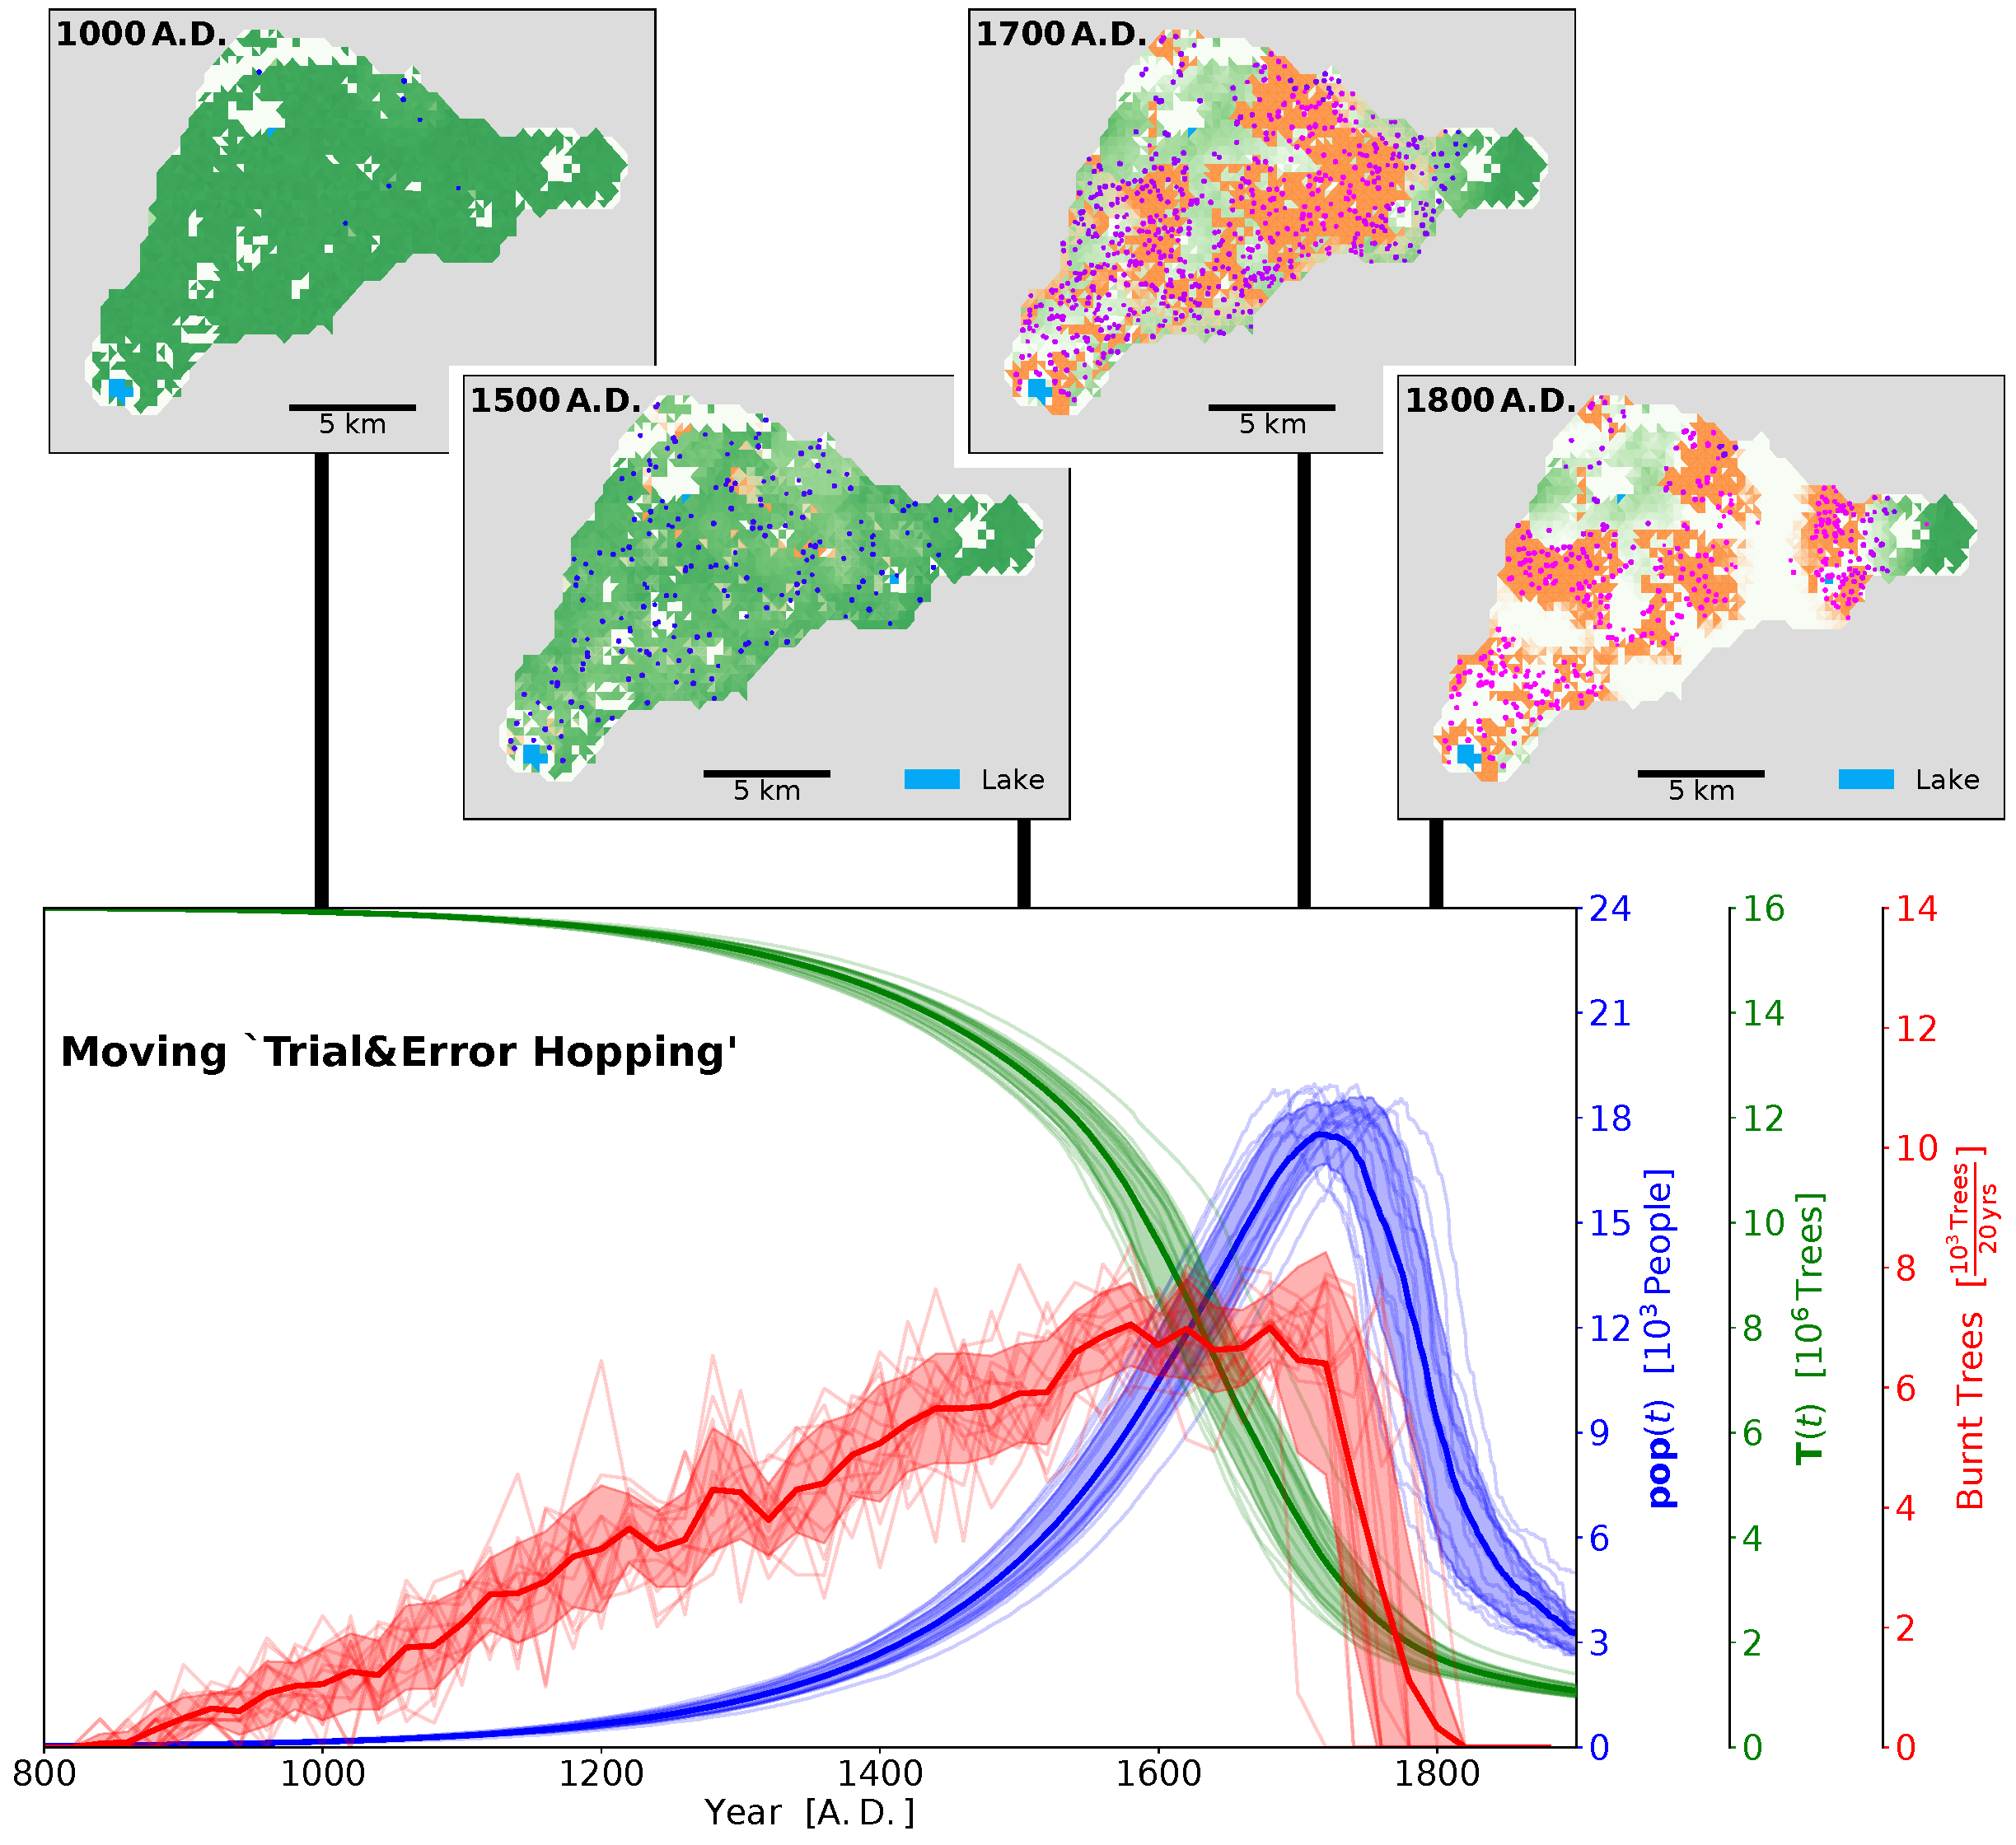
\includegraphics[width=1\textwidth]{images/Results/Moving/alphaHopping_EnsembleStatistics+Panels}
	\caption{Moving strategy `Trial\&Error Hopping'.}
	\label{fig:hop}
\end{figure}
The four different moving strategies presented here (Standard, Only Resources, Optimal Location and Trial\&Error Hopping) do not only change the spatial pattern but also influence the overall dynamics of the model and, therefore, can not be simply ignored in the calculation of aggregate variables. 
This is especially apparent for the number of burnt trees.
In particular, if agents do not move according to considerations (`Trial\&Error Hopping' strategy), the overall population dynamics are affected, e.g.\ the decrease after the population size peak becomes steeper.

%\paragraph{Comment on the Moving Module.}
There is, of course, substantial freedom in modelling the evaluations of potential new locations and the decision making process related to moving.
The framework is therefore kept flexible and other assumptions or new categories can easily be added or adjusted.
There has not been any comparable approach for Easter Island society yet.
In the ABM simulating the Anasazi people by \citet{Axtell2002} and \citet{Janssen2009}, agents that relocate their farms (and settlements) consider all eligible cells that fulfil certain nutrient production and water availability criteria and then choose the cell closest to the previous location.
In general, I use a similar rationale but implement a more elaborate evaluation process that in particular introduces non-linear, continuous rather than binary evaluation criteria, more/different penalty categories and stochasticity in the decision making process.  
As shown, this procedure (in the standard run configuration) yields moving patterns that are consistent with plausible reconstructions on Easter Island history.






% !TEX root=frame_thesis.tex

\chapter{Conclusions}

Many studies in general and throughout the field of Easter Island research in particular have emphasized the importance of heterogeneous, spatial and stochastic considerations and the consequent constraints imposed on modelling societies.
E.g.\ \citet{Bousquet2004} describe the importance of modelling spatial and discrete in general, \citet{Merico2017} points out gaps of Easter Island modelling with respect to these aspects, \citet{Rull2020} argues that the spatio-temporal dynamics on Easter Island is heterogeneous, and \citet{Stevenson2015} among many other studies argues against an island-wide homogeneous dynamics before European contact.
However, surprisingly very little effort has been put into quantifying such qualitative assessments.
Here, I provided a first approach of a spatially explicit and realistic, stochastic and discrete model in the form of an Agent Based Model of human-resource interaction on Easter Island prior to European contact that simulates the settling of household agents interacting with a spatially explicit local environment. 

The model has several shortcomings as mentioned in the Model Description and Discussion:
First, there are numerous parameters describing both the environment and the agent behaviour which are subject to uncertainties or even chosen by instinct as there is either not sufficient or no data at all.
Agents in the model act entirely myopic (e.g.\ in the clearing of space for farming), self-centred and their harvest behaviour simply aims to maximise population size growth in each year regardless of future considerations or sustainability norms. 
So far, all agents have homogeneous conditions (e.g.\ the same penalty evaluation or tree preference adaption strategy or minimum tree preference).
There is neither agent-agent interaction, cooperation, trade nor any advanced economic or social structure (such as taboos) above the household level. 
%Agents also do not plan ahead e.g.\ when it comes to using the trees before burning them to clear sites for farming.
Further caveats include the rather simplified population growth module depending on resource harvest for a single agent, the oversimplified erosion process and assumptions of constant yield from a farming site regardless of e.g.\ labour considerations or climatic variation.

Despite these numerous shortcomings, especially the agent behaviour can be sufficiently well constructed through plausible, intuitive anthropogenic rules.
Or, as \citet{Kohler2000} put it: "Agent construction at this point is more art than science".
The impacts of some of the other shortcomings are explored by testing different experiments and sensitivity of parameters.

The standard run of the ABM presented here shows a boom and bust dynamics, i.e.\ an exponential growth of the population size, a short phase of peak population and a decrease (with rate in the order of the initial growth) thereafter.
This corresponds to the classical ecocidal narrative of Easter Island history by \citet{Brander1998}, \citet{Diamond2011} or \citet{Bahn2017}.
Results that are more consistent with alternative population dynamic narratives, however, can be obtained by changing only a few parameters, in particular the tree regrowth and agricultural quality of the soil on Easter Island.



Next to the general proof of concept the ABM yields three major results:
Firstly, the population decrease in the standard run is caused by the lack of either farming sites or trees in all potential locations on Easter Island but not an island-wide lack of either of these resources.
Secondly, the model shows how spatial considerations of microscopic units constrain the population dynamics overall and thus are computationally irreducible.
E.g.\ varying the resource search radii or having different moving strategies impact the total number of burnt trees, deforestation, and population size.
Thirdly, slightly different strategies to adapt to the environmental degradation lead to different outcomes overall in the model. 
In particular, the best strategy is to quickly decrease the tree preference, i.e.\ the dependence on a non-renewable resource. While this fast transition leads to more trees overall being burnt to clear land, the population size throughout the time period and even the total number of trees eventually are larger. 
%the model shows that allowing for individual and stochastic decisions (e.g.\ in the adaption strategy in relation to the tree preference and the penalty evaluation in the moving process) can lead to surprising aggregate behaviour.
Fourth and finally, this ABM provides, for the first time, quantitative regional variations in the dynamics of population, tree, and agriculture density, which are in many aspects consistent with qualitative descriptions in the literature (of the ecocidal narrative).
The regional dynamics are found to be very heterogeneous in shape and timings and far from a uniform island wide collapse.
Such spatio-temporal patterns emerge from the assumption of discrete, non-ergodic, stochastic and individual decision making processes of the agents.
%They are consistent in many aspects with qualitative descriptions of spatially explicit, natural and settlement history on Easter Island in the literature (of the ecocidal view).
An important implication of these results is that data obtained from single sites and used for an island wide interpretation of the population dynamics should be considered with caution.
In general, the model gives a novel view on Easter Island by adding a spatial impression to the ongoing debate about the island wide overall population dynamics before European contact.

%The ABM presented in this thesis includes various processes and parameters motivated not so much by data or proven relations but by intuitive assumptions from everyday experience.
%"Agent construction at this point is more art than science" \citep{Kohler2000}.

A major advantage of Agent Based Modelling is its flexibility and that the complexity of the model does not need to be known a priori \citep{Bonabeau2002}.
The presented model, can easily incorporate more, different or less modules, rules or processes.
Further research, e.g.\ on emergent social institutions as suggested in the Discussion here, is, thus, strongly encouraged to use this or similar approaches to better understand the history of Easter Island before European contact and, thereby, to further explore the general concept of overpopulation in a world with limited resources.



\printbibliography[heading=bibintoc]

\appendix

% !TEX root=frame_thesis.tex

\chapter{More Details of the Model} \label{sec:APPpopgrowth}
\FloatBarrier
\begin{figure}[h]
	\centering
	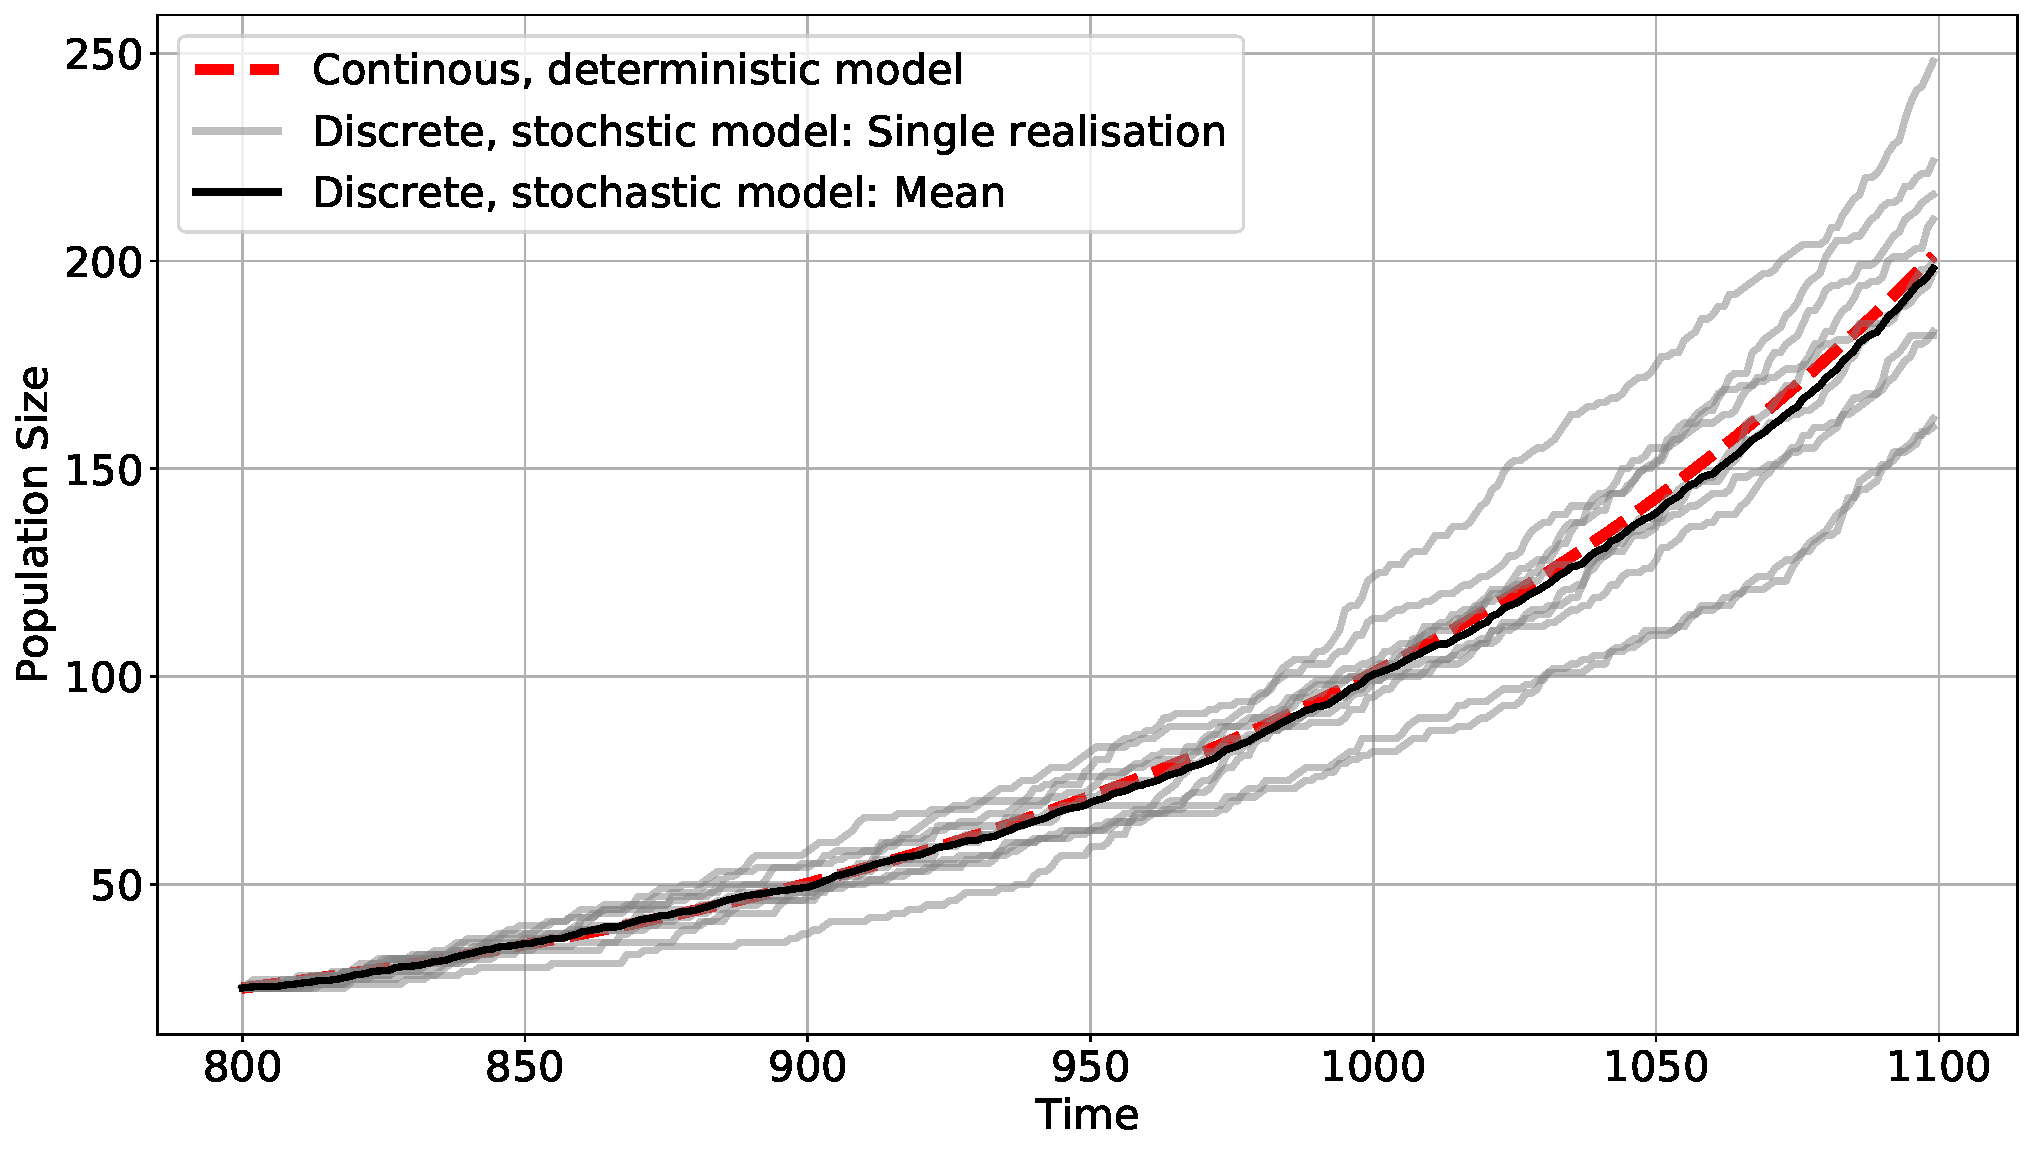
\includegraphics[width=\textwidth]{images/RealisationsOfPopGrowth.pdf}
	\caption{Realisations (and the mean) of the discrete, stochastic population growth model (assuming $H_{\rm i}(t) = 1$ for all $t$ here. In comparison, the continuous exponential growth. The growth rate is $g(H_{\rm i}(t)=1)=1.007$, as in the standard setting of the model.}
	\label{fig:realisationsofpopgrowth}
\end{figure}


\chapter{More Results}
\FloatBarrier
\section{Additional Results: Standard Run}

\begin{figure}[h]
	\centering
	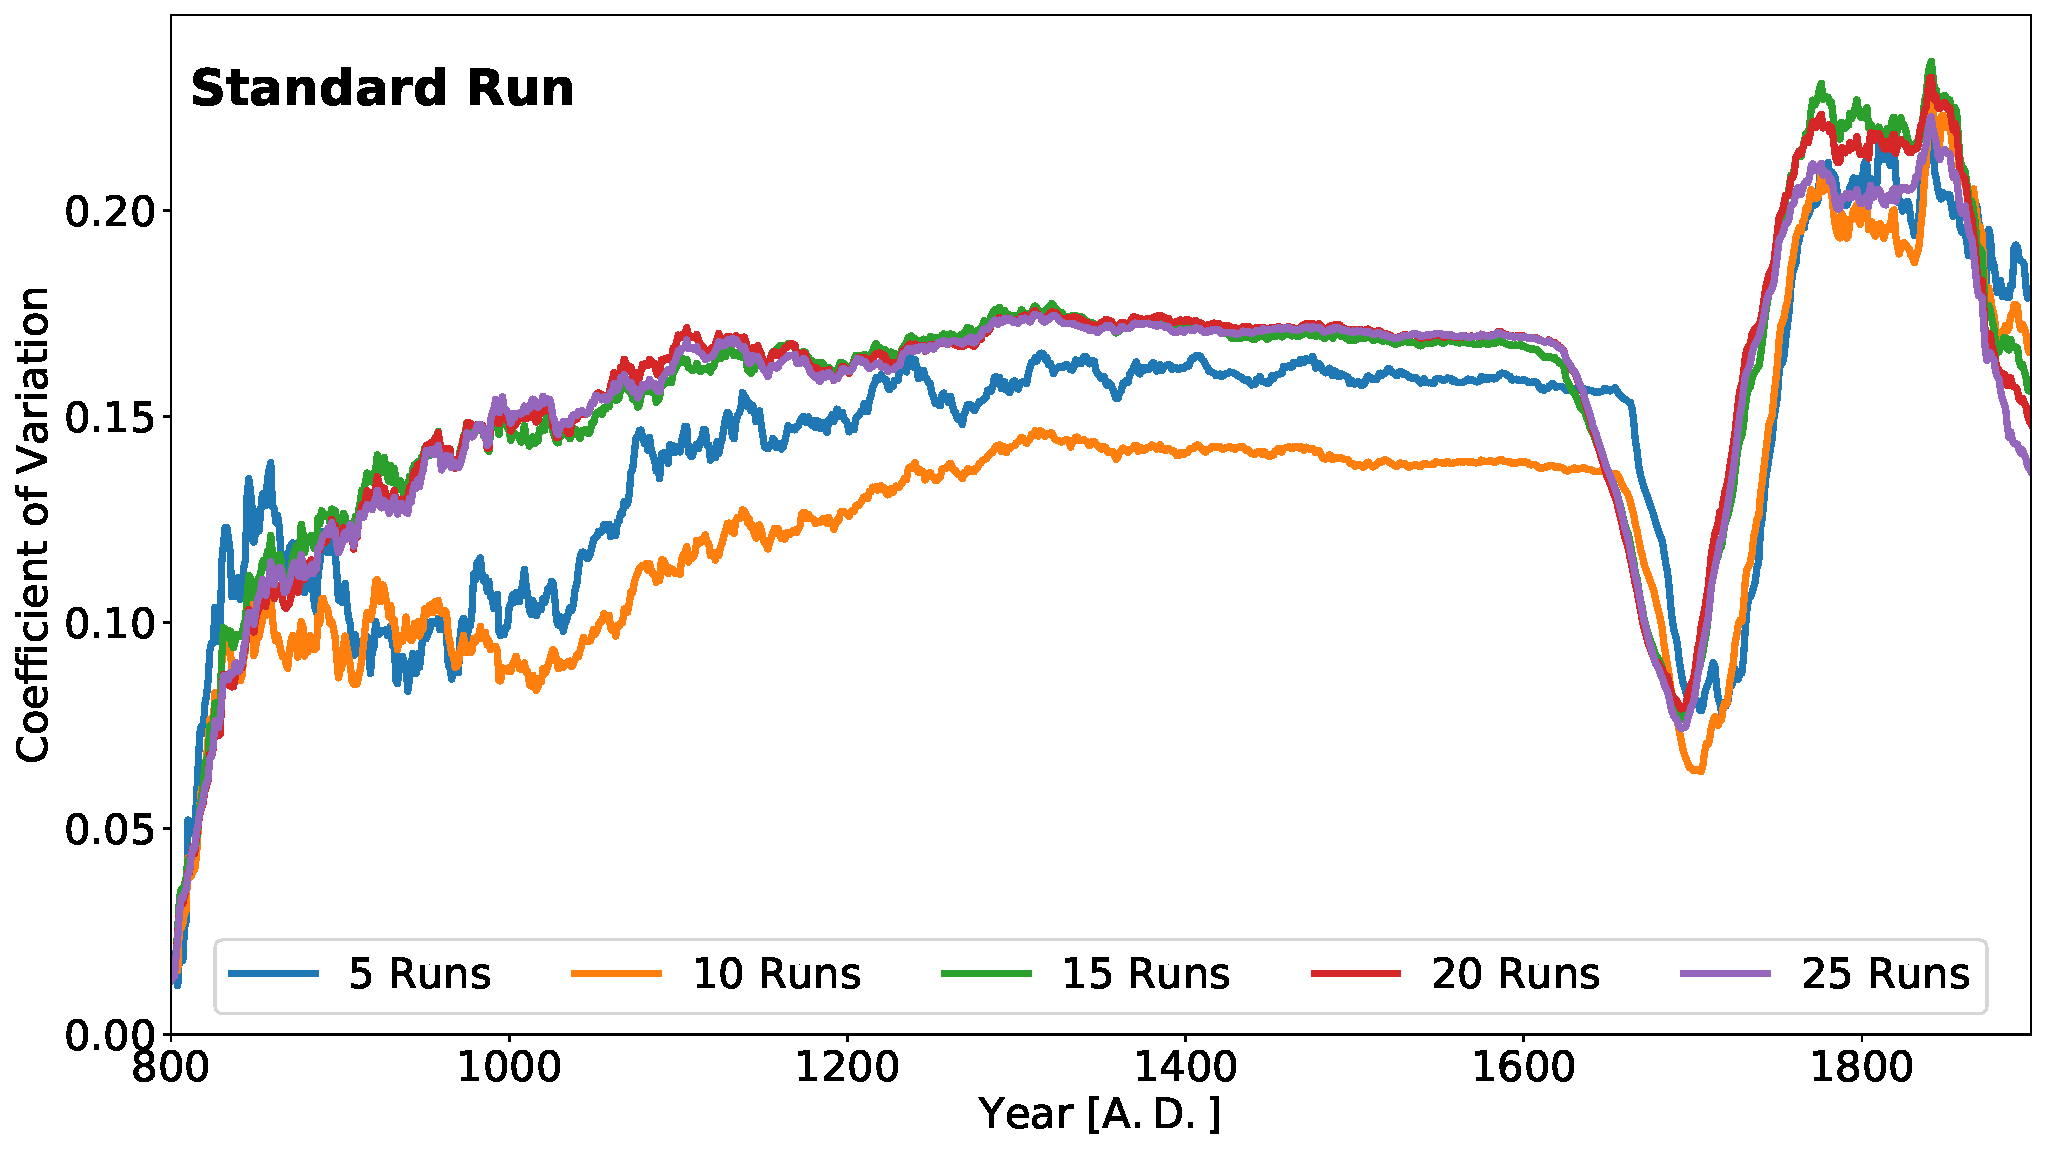
\includegraphics[width=\textwidth]{images/Results/Standard/CoeffOfVariation}
	\caption{The coefficient of variation of ensembles of 5 to 25 runs for the Standard run over time. For more than 15 runs, the coefficient of variation does not change significantly and, thus, this provides a good ensemble size}
	\label{fig:coeffofvariation}
\end{figure}


\begin{figure}[h]
	\centering
	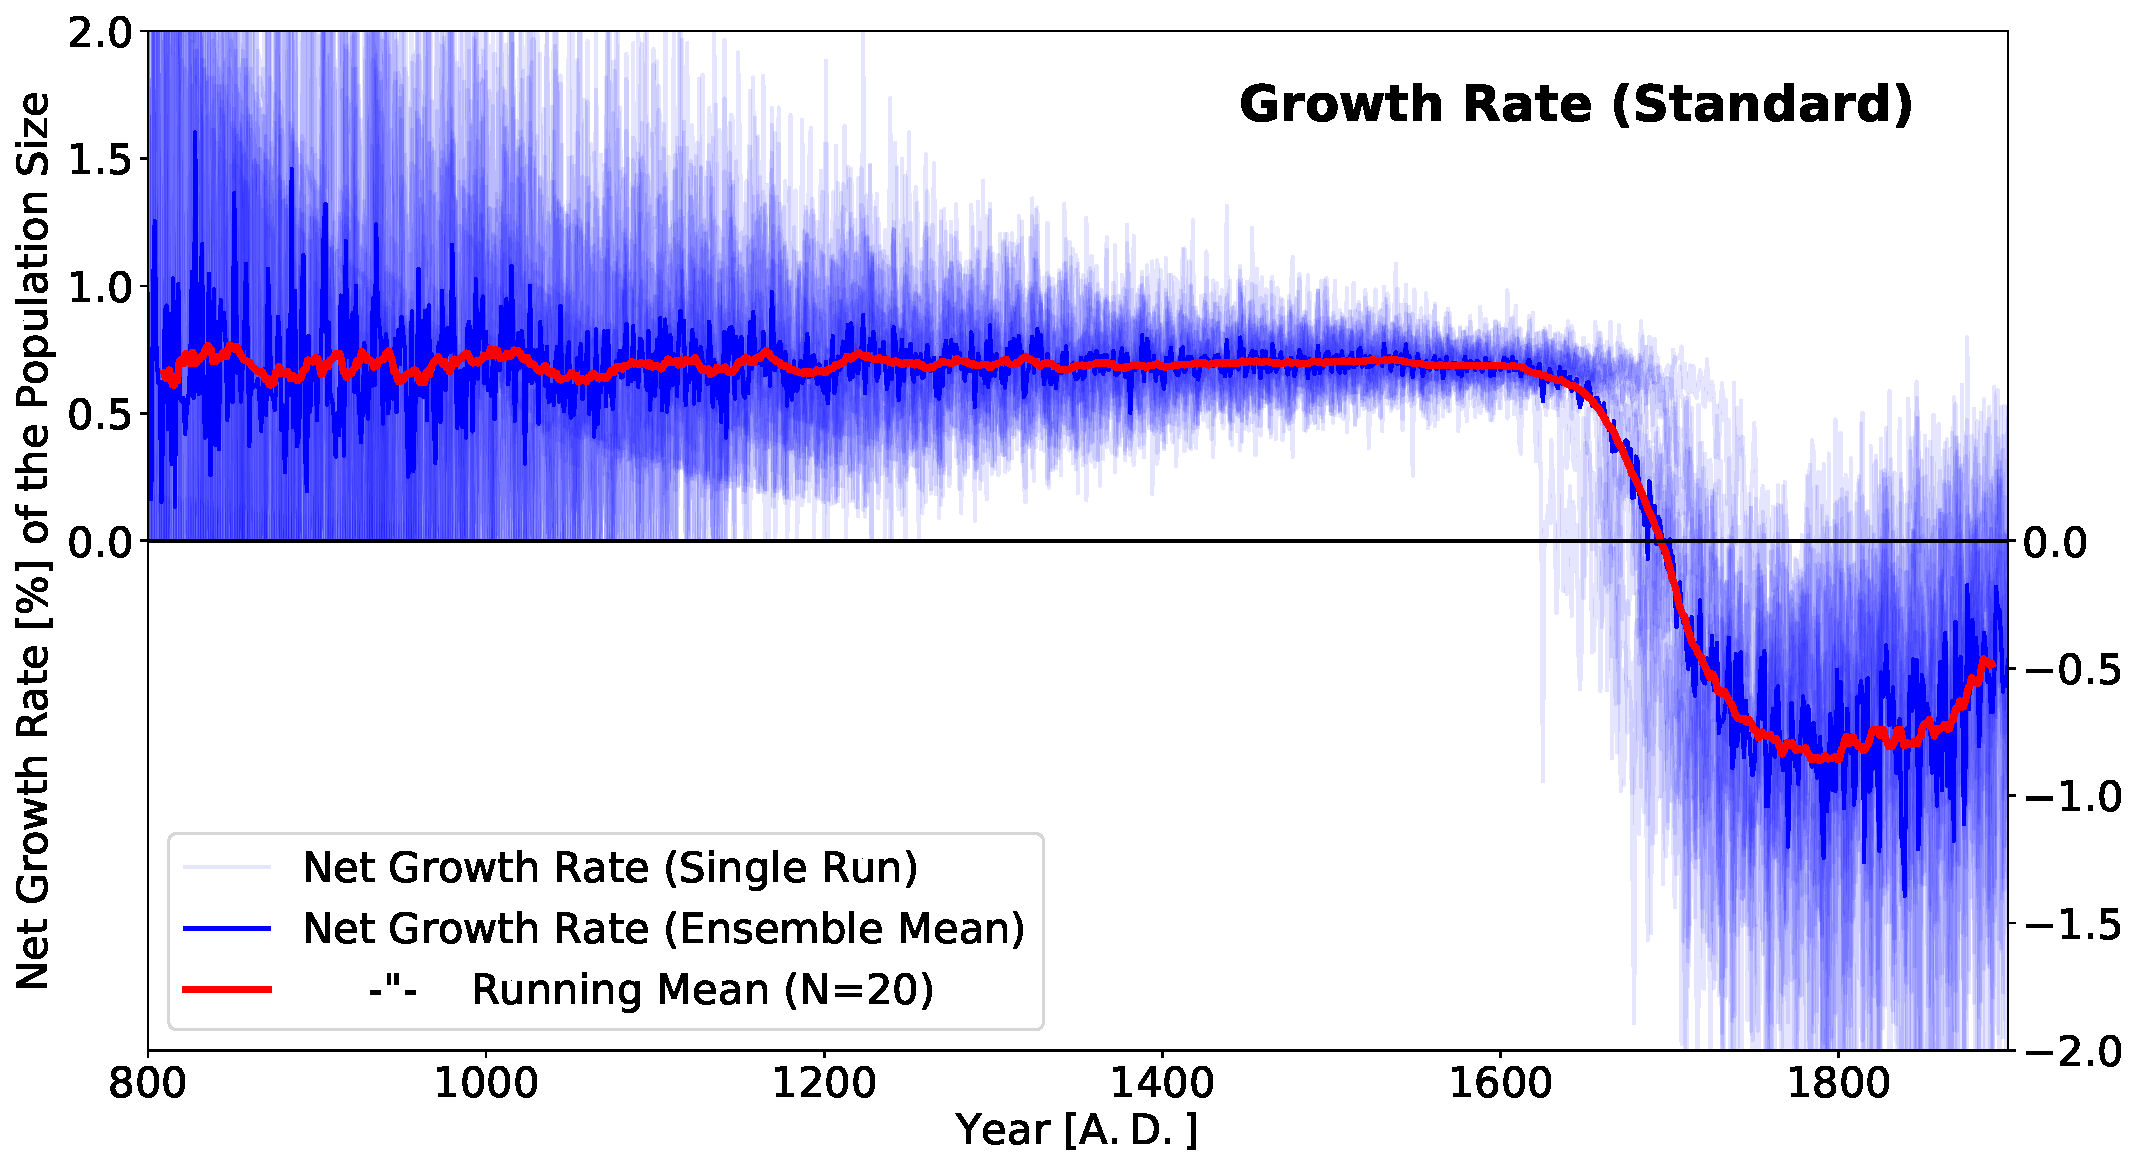
\includegraphics[width=1.0\linewidth]{images/Results/Standard/NetGrowthRate}
	\caption{Ensemble of five Standard runs. The net population growth rate is shown as the mean of the ensemble (blue) and, for easier visibility, as a running mean (red).} 
	\label{fig:app:STDnetgrowthrate}
\end{figure}
\FloatBarrier
\section{Clustering the Agents}
\begin{figure}[h]
	\centering
	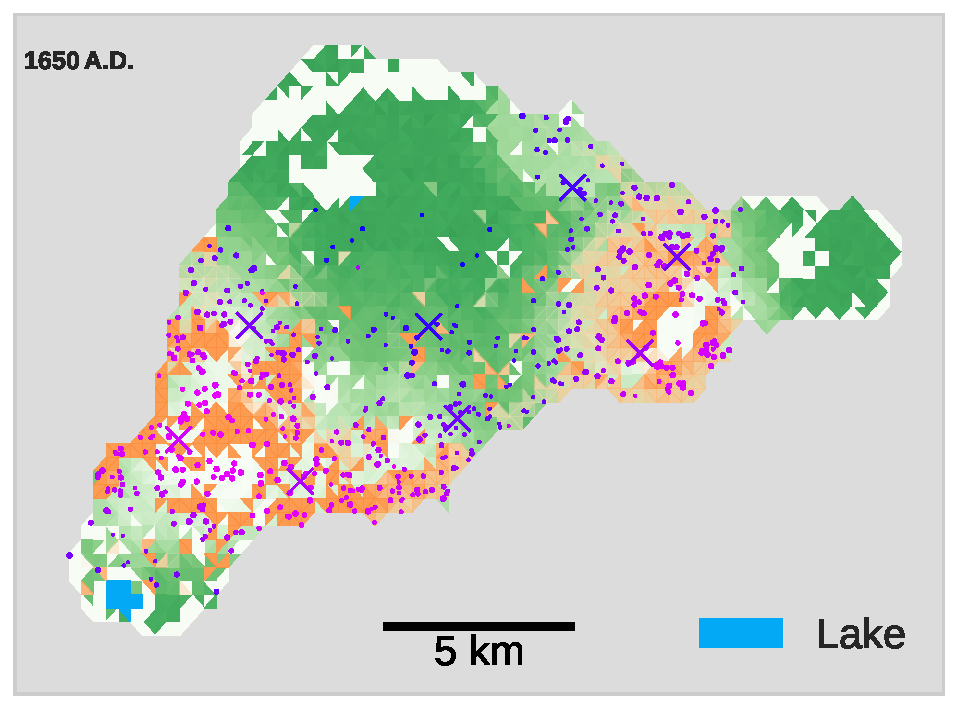
\includegraphics[width=1\linewidth]{images/ClusterSTDS1650}
	\caption{The map shows one realisation of the Standard run. The agents are assigned to clusters with midpoints (crosses) by a k-Means algorithm of the three dimensional state vectors $\left( x_{\rm i}, y_{\rm i}, T_\text{Pref, i} \right)(t)$ for agent $i$ in the year $1650\, {\rm A.D.}$.}
	\label{fig:clusterstds1650}
\end{figure}

\FloatBarrier
\section{Additional Results: Variation in the Agents' Strategy of Adapting the Tree Preference}
\begin{figure}[h]
	\centering
	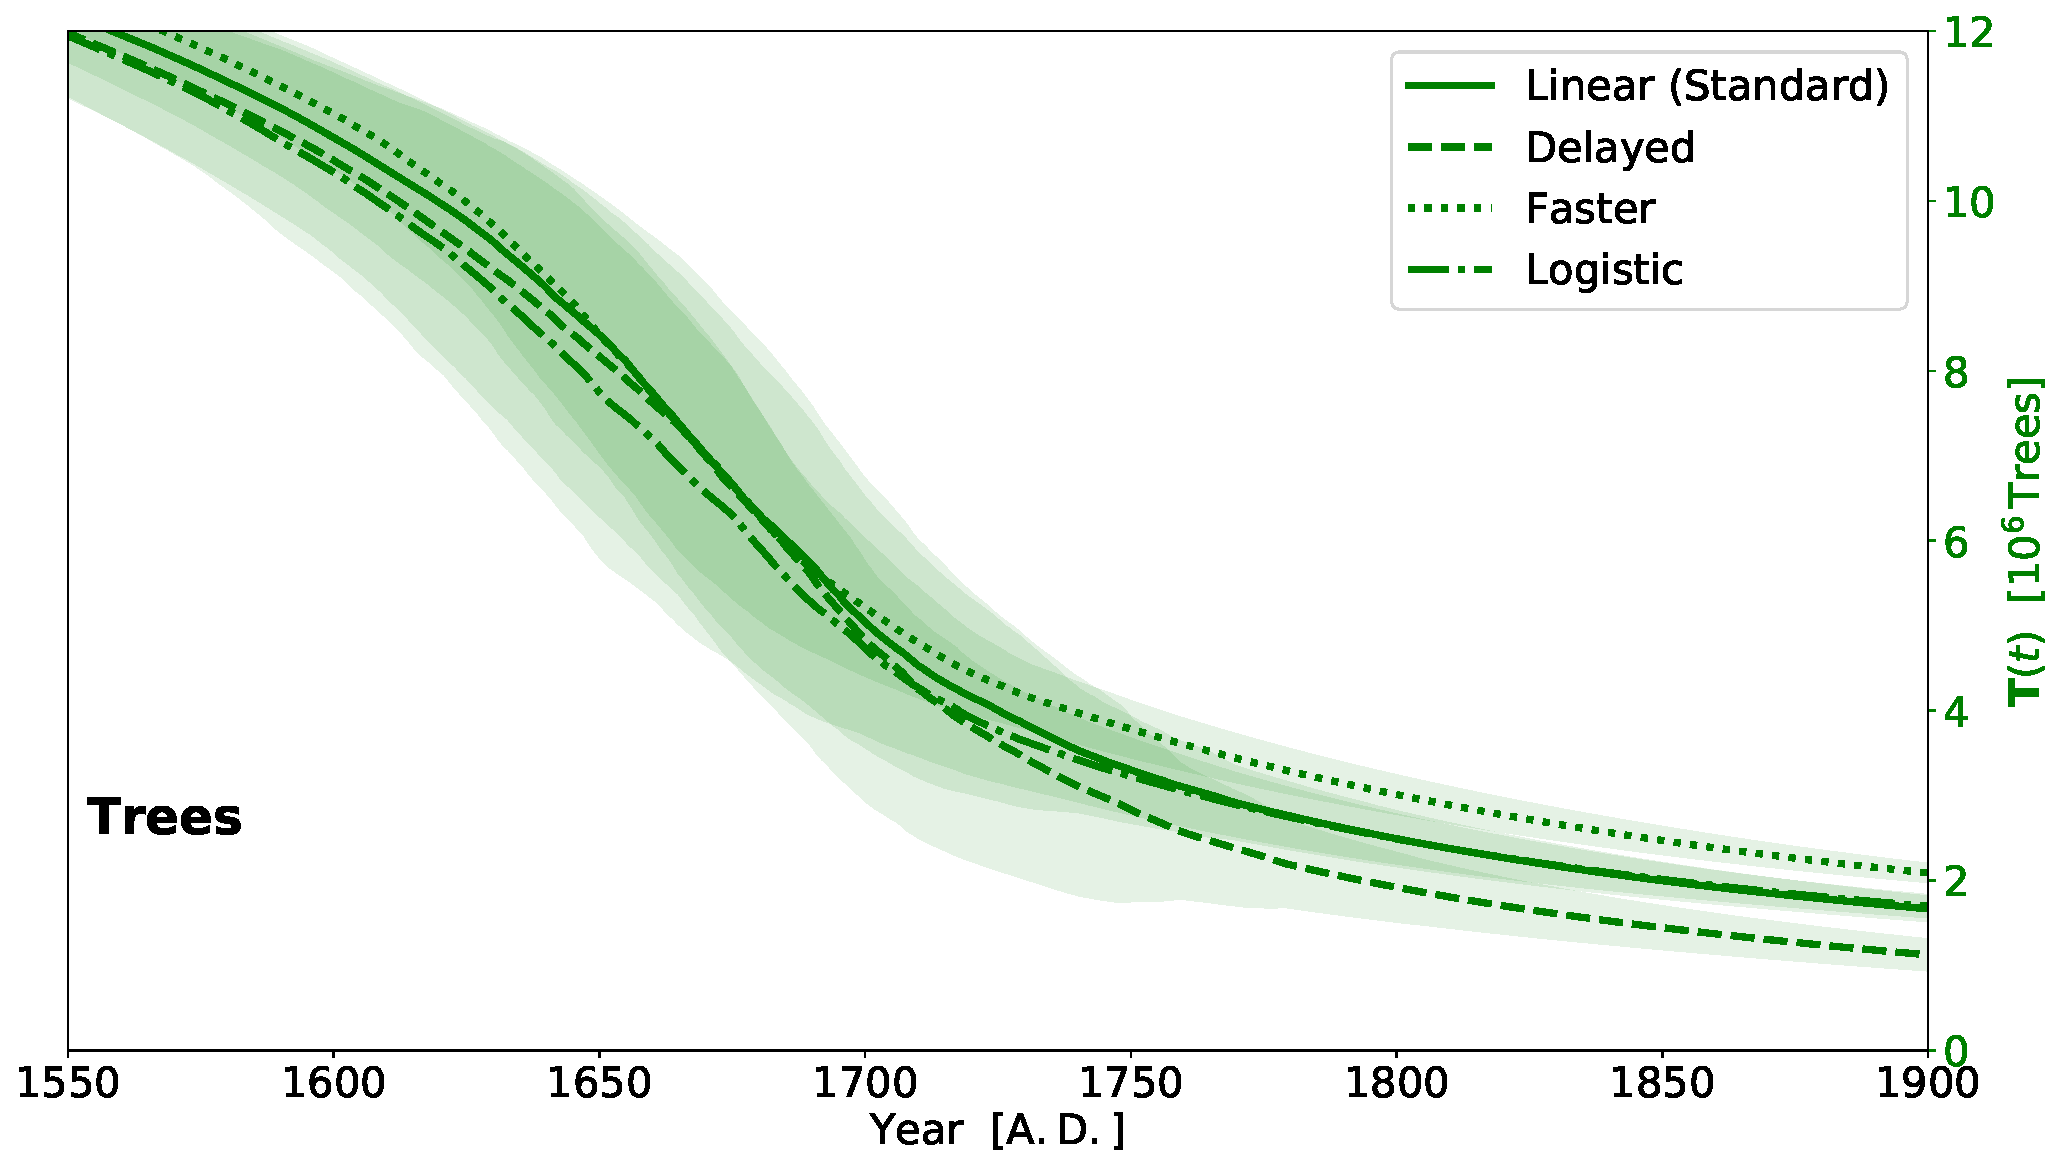
\includegraphics[width=1\linewidth]{images/Results/TPref/TPrefAdaption_Trees}
	\caption{Number of Burnt Trees in the four different Adoption strategies of the tree preference.}
	\label{fig:tprefadaptiontrees}
\end{figure}

\begin{figure}[h]
	\centering
	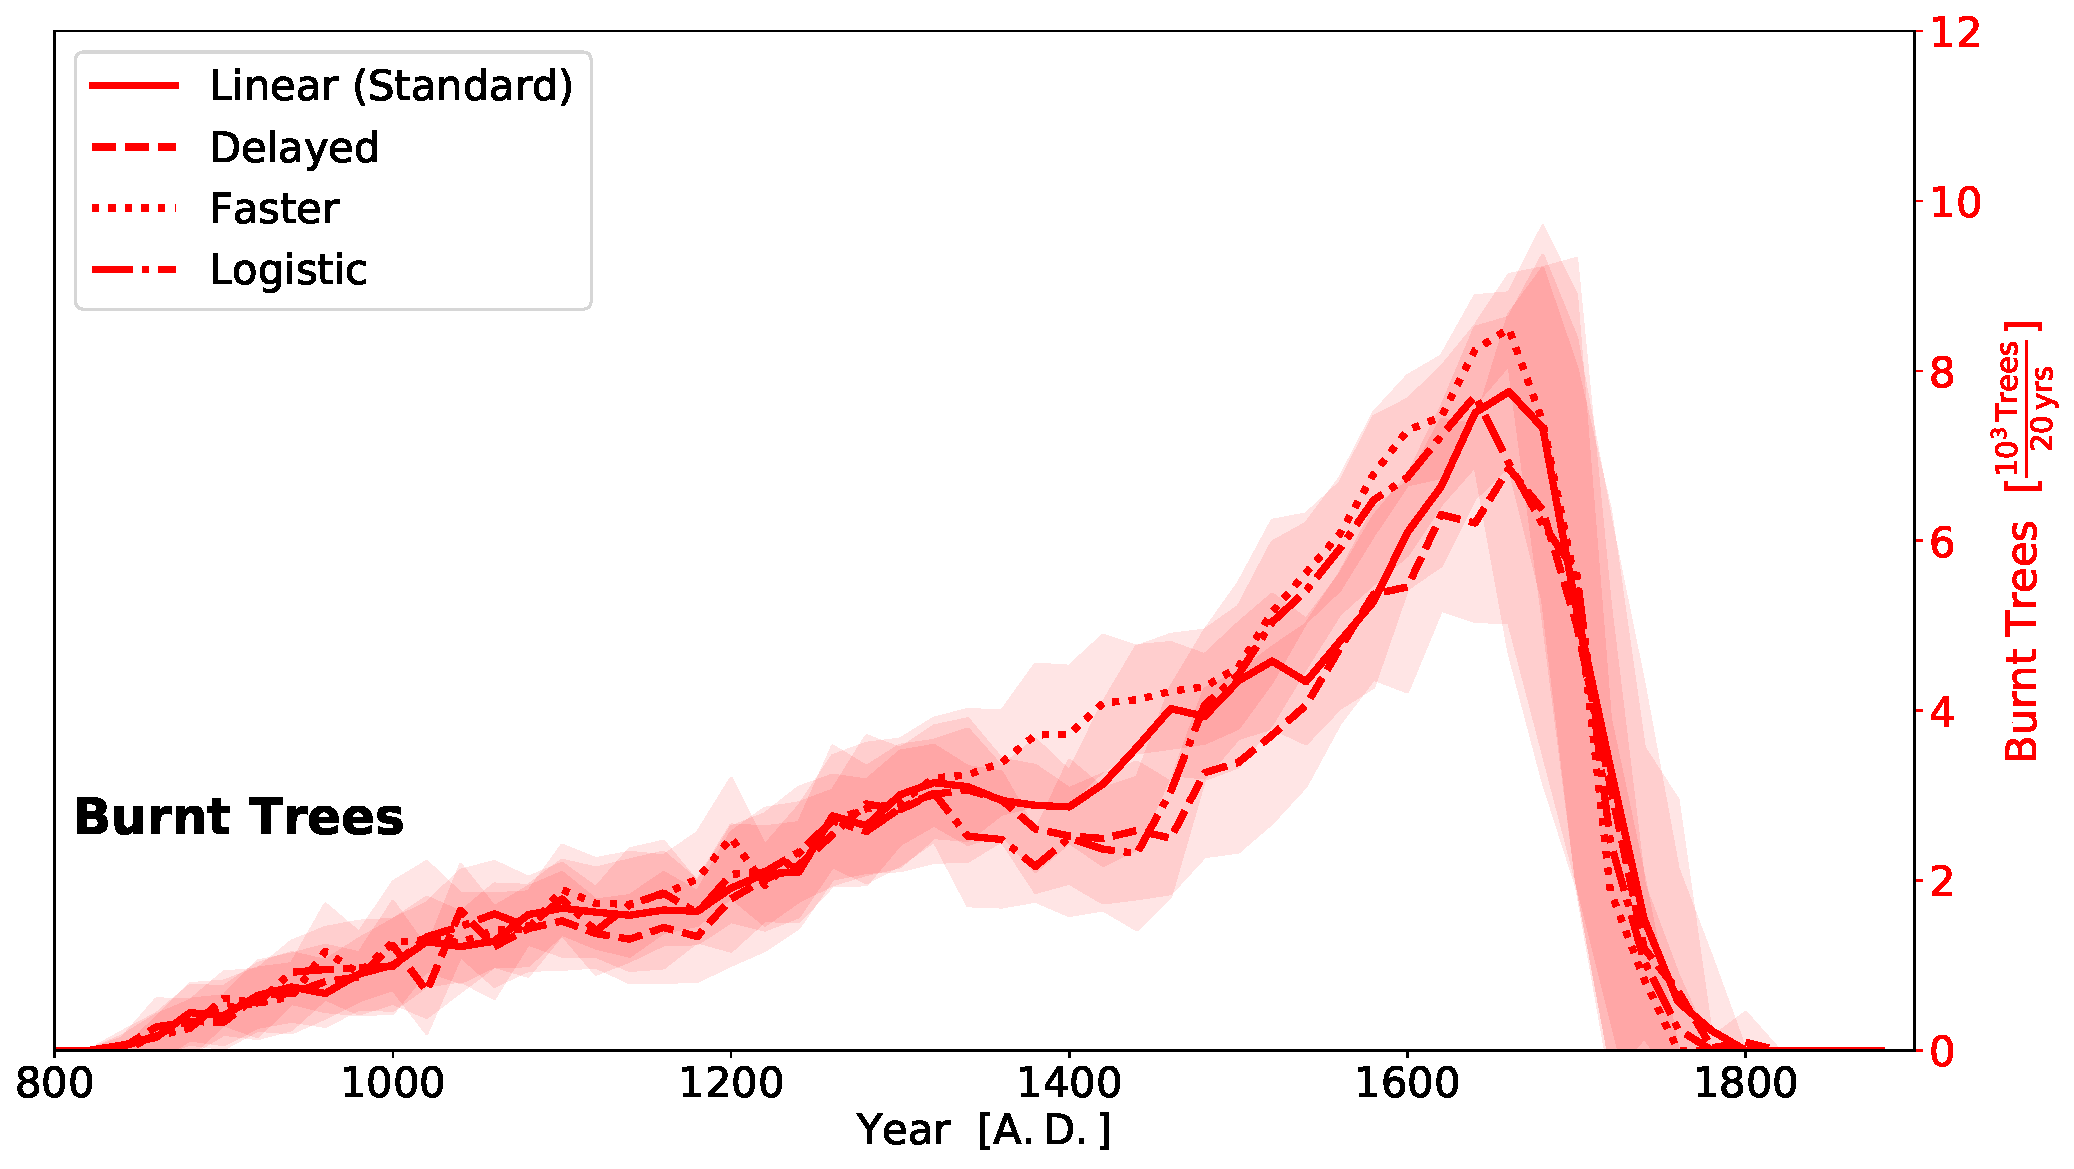
\includegraphics[width=1.0\linewidth]{images/Results/TPref/TPrefAdaption_BurntTrees}
	\caption{Number of Burnt Trees in the four different Adoption strategies of the tree preference.}
	\label{fig:tprefadaptionburnttrees}
\end{figure}
\tailmatter

\end{document}
